\documentclass[,a4paper]{article}
\usepackage[ngerman]{babel}
\usepackage{geometry}
\geometry{a4paper,left=35mm,right=35mm, top=25mm, bottom=25mm}
\usepackage[T1]{fontenc}
\usepackage{lmodern}
\usepackage{longtable}
\usepackage{amssymb,amsmath}
\usepackage{ifxetex,ifluatex}
\usepackage{fixltx2e} % provides \textsubscript
% use microtype if available
\IfFileExists{microtype.sty}{\usepackage{microtype}}{}
\ifnum 0\ifxetex 1\fi\ifluatex 1\fi=0 % if pdftex
  \usepackage[utf8]{inputenc}
\else % if luatex or xelatex
  \usepackage{fontspec}
  \ifxetex
    \usepackage{xltxtra,xunicode}
  \fi
  \defaultfontfeatures{Mapping=tex-text,Scale=MatchLowercase}
  \newcommand{\euro}{€}
\fi
\usepackage{color}
\usepackage{fancyvrb}
\newcommand{\VerbBar}{|}
\newcommand{\VERB}{\Verb[commandchars=\\\{\}]}
\DefineVerbatimEnvironment{Highlighting}{Verbatim}{commandchars=\\\{\}}
% Add ',fontsize=\small' for more characters per line
\newenvironment{Shaded}{}{}
\newcommand{\KeywordTok}[1]{\textcolor[rgb]{0.00,0.44,0.13}{\textbf{{#1}}}}
\newcommand{\DataTypeTok}[1]{\textcolor[rgb]{0.56,0.13,0.00}{{#1}}}
\newcommand{\DecValTok}[1]{\textcolor[rgb]{0.25,0.63,0.44}{{#1}}}
\newcommand{\BaseNTok}[1]{\textcolor[rgb]{0.25,0.63,0.44}{{#1}}}
\newcommand{\FloatTok}[1]{\textcolor[rgb]{0.25,0.63,0.44}{{#1}}}
\newcommand{\CharTok}[1]{\textcolor[rgb]{0.25,0.44,0.63}{{#1}}}
\newcommand{\StringTok}[1]{\textcolor[rgb]{0.25,0.44,0.63}{{#1}}}
\newcommand{\CommentTok}[1]{\textcolor[rgb]{0.38,0.63,0.69}{\textit{{#1}}}}
\newcommand{\OtherTok}[1]{\textcolor[rgb]{0.00,0.44,0.13}{{#1}}}
\newcommand{\AlertTok}[1]{\textcolor[rgb]{1.00,0.00,0.00}{\textbf{{#1}}}}
\newcommand{\FunctionTok}[1]{\textcolor[rgb]{0.02,0.16,0.49}{{#1}}}
\newcommand{\RegionMarkerTok}[1]{{#1}}
\newcommand{\ErrorTok}[1]{\textcolor[rgb]{1.00,0.00,0.00}{\textbf{{#1}}}}
\newcommand{\NormalTok}[1]{{#1}}
\usepackage{ctable}
\usepackage{float} % provides the H option for float placement
\usepackage{graphicx}
% We will generate all images so they have a width \maxwidth. This means
% that they will get their normal width if they fit onto the page, but
% are scaled down if they would overflow the margins.
\makeatletter
\def\maxwidth{\ifdim\Gin@nat@width>\linewidth\linewidth
\else\Gin@nat@width\fi}
\makeatother
\let\Oldincludegraphics\includegraphics
\renewcommand{\includegraphics}[1]{\Oldincludegraphics[width=\maxwidth]{#1}}
\ifxetex
  \usepackage[setpagesize=false, % page size defined by xetex
              unicode=false, % unicode breaks when used with xetex
              xetex]{hyperref}
\else
  \usepackage[unicode=true]{hyperref}
\fi
\hypersetup{breaklinks=true,
            bookmarks=true,
            pdfauthor={OParl Team - http://oparl.org/},
            pdftitle={OParl Schnittstellen-Spezifikation (Branch backtojson)},
            colorlinks=true,
            urlcolor=blue,
            linkcolor=magenta,
            pdfborder={0 0 0}}
\setlength{\parindent}{0pt}
\setlength{\parskip}{6pt plus 2pt minus 1pt}
\setlength{\emergencystretch}{3em}  % prevent overfull lines
\setcounter{secnumdepth}{0}

\title{OParl Schnittstellen-Spezifikation (Branch ``backtojson'')}
\author{OParl Team - \url{http://oparl.org/}}
\date{}

\begin{document}
\maketitle

Lizenz: Creative Commons CC-BY-SA

\section{Einleitung}\label{einleitung}

Dieses Dokument enthält die Spezifikation des OParl
Schnittstellen-Standards für parlamentarische
Informationssysteme\footnote{In Deutschland hat sich auf kommunaler
  Ebene der Begriff ``Ratsinformationssystem'' etabliert. OParl ist in
  seiner Anwendung jedoch nicht auf Gemeinderäte eingeschränkt und
  verwendet daher den Begriff ``parlamentarisches Informationssystem''.}
darstellen. Es dient damit als Grundlage für die Implementierung von
OParl-konformen Server- und Clientanwendungen.

\subsection{Was ist OParl in Kürze?}\label{was-ist-oparl-in-kuxfcrze}

OParl ist die Gruppierung, die Initiator und Herausgeber der
vorliegenden Spezifikation ist. An OParl wirken Verbände,
Zivilgesellschaftliche Organisationen und Initiativen und
Software-Anbieter sowie interessierte Einzelpersonen mit.

Die vorliegende Spezifikation beschreibt den OParl-Standard. Dieser
definiert eine Webservice-Schnittstelle, die den anonymen und lesenden
Zugriff auf öffentliche Inhalte aus parlamentarischen
Informationssystemen ermöglicht. Wie der Name ``Webservice'' ausdrückt,
setzt diese Schnittstelle auf dem World Wide Web auf. Sie ermöglicht,
dass parlamentarische Informationen maschinenlesbar als Offene Daten
(Open Data) veröffentlicht werden.

Die vorliegende Version ist die erste verabschiedete Version der
Spezifikaiton zum OParl-Standard.

\subsection{Zielsetzung von OParl}\label{zielsetzung-von-oparl}

OParl richtet sich an verschiedene Nutzergruppen und Stakeholder:

\begin{itemize}
\itemsep1pt\parskip0pt\parsep0pt
\item
  Verwaltung und politische Gremien in Gebietskörperschaften
\item
  Bürger, politische Parteien und Organisationen
\item
  Open-Data-Initiativen
\item
  Wissenschaftler
\item
  Anbieter von Server- und Softwareprodukten
\item
  Anbieter von Linked-Data-Plattformen oder -Services
\end{itemize}

Die Gründe, warum Betreiber von parlamentarischen Informationssystemen
den Zugriff darauf über eine standardisierte Schnittstelle ermöglichen
sollten oder möchten, können vielfältig sein und je nach Nutzergruppe
unterschiedlich.

Ein zentrales Argument für Verwaltung und politische Gremieni, sei es in
Gebietskörperschaften oder auf Landes- oder Bundesebene, ist die
Verpflichtung der Parlamente gegenüber der Bevölkerung, diese über die
Fortschritte der parlamentarischen Arbeit zu informieren und auf dem
Laufenden zu halten. Ein erster Schritt, der Bevölkerung Einblicke in
die Arbeit und Zugriff auf Dokumente zu gewähren, ist vielerorts in den
letzten Jahren durch Einführung von Ratsinformationssystemen mit
anonymem, lesenden Zugriff über das World Wide Web gemacht worden.

Die damit eingeschlagene Richtung konsequent weiter zu gehen, bedeutet,
die Daten der parlamentarischen Informationssystemen gänzlich offen zu
legen, sofern die Inhalte es erlauben. Es bedeutet, die Daten und
Inhalte so universell weiterverwendbar und so barrierearm wie möglich
anzubieten, dass jegliche weitere Verwendung durch Dritte technisch
möglich ist. Der seit einiger Zeit etablierte Begriff für dieses Prinzip
heißt ``Open Data''.

Open-Data-Initiativen können unter Rückgriff auf RIS mit
OParl-Schnittstelle einfacher Dokumente und Daten aus unterschiedlichen
Gebietskörperschaften in Open-Data-Katalogen verzeichnen und so
einfacher auffindbar machen für die Weiterverwendung durch Dritte.

Bürgerinnen und Bürger, politische Parteien und zivilgesellschaftliche
Organisationen können einfacher auf Inhalte parlamentarischer
Informationssysteme zugreifen und diese entsprechend ihren Interessen
aufbereiten. Dies können beispielsweise Visualisierungen von enthaltenen
Daten, die Anreicherung von Informationsangeboten für spezielle
Nutzergruppen oder die Schaffung von Benutzeroberflächen mit besonderen
Funktionen für verschiedene Endgeräte sein.

Das Interesse an parlamentarischen Informationen und an Anwendungen, die
diese nutzbar und auswertbar machen, ist offensichtlich vorhanden. Die
Entwickler der alternativen Ratsinformationssysteme wie Frankfurt
Gestalten\footnote{Frankfurt Gestalten:
  \url{http://www.frankfurt-gestalten.de/}}, Offenes Köln\footnote{Offenes
  Köln: \url{http://offeneskoeln.de/}} oder der
OpenRuhr:RIS-Instanzen\footnote{OpenRuhr:RIS:
  \url{http://openruhr.de/openruhrris/}} wissen zu berichten, wie viel
Interesse den Projekten gerade aus Orten entgegen gebracht wird, in
denen derartige Systeme noch nicht verfügbar sind.

Die Anwendungsmöglichkeiten für parlamentarische Informationen, wenn sie
über eine Schnittstelle schnell und einfach abgerufen werden können,
sind vielfältig. Beispiele sind:

\begin{itemize}
\itemsep1pt\parskip0pt\parsep0pt
\item
  Apps für den Abruf auf mobilen Endgeräten
\item
  Möglichkeiten zur Wiedergabe für Nutzerinnen und Nutzer mit
  Beeinträchtigung des Sehvermögens
\item
  Alternative und erweiterte Suchmöglichkeiten in Inhalten
\item
  Auswertung und Analyse von Themen, Inhalten, Sprache etc.
\item
  Benachrichtigungsfunktionen beim Erscheinen bestimmte Inhalte
\end{itemize}

Die Standardisierung dieses Zugriffs über die Grenzen einzelner Systeme
hinweg erlaubt zudem, diese Entwicklungen grenzüberschreitend zu denken.
Damit steigt nicht nur die potenzielle Nutzerschaft einzelner
Entwicklungen. Auch das Potenzial für Kooperationen zwischen
Anwendungsentwicklern wächst.

Für Wissenschaftler, die z. B. an vergleichenden Untersuchungen zu
Vorgängen in verschiedenen Gebietskörperschaften interessiert sind,
ergeben sich ebenso vielfältige Möglichkeiten über mehrere RIS-Instanzen
hinweg auf entsprechende Informationen zuzugreifen und diese so
einfacher in ihre Analysen einzubeziehen.

Darüber hinaus sind auch Motivationen innerhalb von Organisationen und
Körperschaften erkennbar. So sollen parlamentarische Informationssysteme
vielerorts in verschiedenste Prozesse und heterogene Systemlandschaften
integriert werden. Durch eine einheitliche Schnittstelle bieten sich
effiziente Möglichkeiten zur Integration der Daten in anderen Systeme,
wie beispielsweise Web-Portale.

Anbieter von Server- und Softwareprodukten, die RIS-Lösungen anbieten,
können mit der Implementation der OParl-Schnittstelle ihren Kunden eine
entsprechende einheitliche Schnittstelle anbieten. Für Anbieter von
Linked-Data-Plattformen ergeben sich u. a. Möglichkeiten zur
vereinfachten Zusammenführung und Anreicherung von Inhalten
parlamentarischer Informationssysteme.

Ausführlichere Beschreibungen einiger möglicher Anwendungsszenarien
finden sich im Kapitel \hyperref[nutzungsszenarien]{Nutzungsszenarien}.

\subsection{Transparenz und Beteiligung durch Open
Data}\label{transparenz-und-beteiligung-durch-open-data}

Öffentliche Stellen verfügen über vielfältige Informationen und Daten.
Seit einigen Jahren sind zivilgesellschaftliche Organisationen sowie
Politik und Verwaltung unter dem Schlagwort \emph{Open Data}
international und auch in Deutschland in unterschiedlichem Maße um eine
stärkere Öffnung dieser Daten bemüht\footnote{Eine weltweite Übersicht
  zu Open-Data-Projekten bietet z. B. der Open-Data-Showroom
  \url{http://opendata-showroom.org/de/}}. Bei dem Ansatz Open
Data\footnote{vgl. \url{https://de.wikipedia.org/wiki/Open_data}} geht
es darum, diese Daten so bereitzustellen, dass Dritte diese einfacher
finden und weiterverwenden können.

Die zehn Open-Data-Prinzipien der Sunlight-Foundation\footnote{Ten
  Principles for Opening Up Open Government Information,
  \url{https://sunlightfoundation.com/policy/documents/ten-open-data-principles}}
beschreiben die Offenheit von Datensätzen. Wesentlich dabei sind vor
allem die einfache rechtliche und die technische Offenheit. Bei ersterer
geht es darum, dass Datensätze unter Nutzungsbestimmungen bereitgestellt
werden, die kurz und verständlich formuliert sind und mindestens
jegliche weitere Verwendung inklusive der kommerziellen erlauben, unter
der Voraussetzung, dass bei der Weiterverwendung die Quelle benannt
wird. Bei der technischen Offenheit steht die Bereitstellung von
Datensätzen in möglichst maschinenlesbaren Formaten im Vordergrund. Dies
bedeutet, stärker strukturierte Datensätze sind in der Bereitstellung zu
bevorzugen. Liegen Daten innerhalb einer Organisation in einer Datenbank
vor, so bietet es sich an, diese soweit möglich über eine
Programmierschnittstelle (API) für Außenstehende bereitzustellen.

Die Erfüllung dieser rechtlichen und technischen Offenheit erlaubt es
Dritten, dies können Bürgerinnen und Bürger, Unternehmen,
Forschungseinrichtungen oder auch andere Verwaltungseinheiten sein, die
Verwaltungsdaten wesentlich unkomplizierter für eigene Vorhaben wie
Anwendungen oder Visualisierungen einzusetzen. Mit dem Ansatz offener
Verwaltungsdaten soll so erstens mehr Transparenz über Prozesse und
Entscheidungen in Politik und Verwaltung erreicht werden. Zweitens
können Dritte auf Grundlage dieser Daten leichter eigene
Geschäftsmodelle verfeinern oder neue entwickeln. Drittens wird es auch
öffentlichen Stellen selbst leichter bereits im öffentlichen Sektor
existierende Daten zu finden und weiterzuverwenden.

Das Prinzip offener Daten bzw. offener Verwaltungsdaten über die
Minimalprinzipien rechtlicher und technischer Offenheit hinaus in die
Tat umzusetzen, erfordert im Einzelfall häufig eine Zusammenarbeit von
Datenbereitstellern und potentiellen Datennutzern. Die bloße
Bereitstellung einer OParl-konformen API wird weder die Einhaltung der
technischen Prinzipien, noch der weiteren Open-Data-Prinzipien
vollständig garantieren. Viele Bestandteile der OParl-Spezifikation, die
einen weitgehend barrierearmen Zugang zu Informationen ermöglichen, sind
optional (Beispiel: Volltexte von Dokumenten über die API abrufbar
machen). Andere Bestandteile, die von Interesse wären, sind noch gar
nicht von OParl abgedeckt (Beispiel: Abstimmungsergebnisse). Grund dafür
ist, dass sich OParl in einem frühen Stadium befindet und primär am
Status Quo der parlamentarischen Informationssysteme ausgerichtet ist.
Es liegt also auch weiterhin an Verwaltung und Politik, durch einen
verantwortungsvollen Umgang mit den Systemen die maximal erreichbare
Transparenz zu bieten. Das fängt bei Dokumentenformaten an (ein PDF mit
digitalem Text weist weit weniger Barrieren auf, als ein gescannter
Brief, der ebenfalls als PDF gespeichert wurde) und hört bei der
verwendeten Sprache auf.\footnote{Weitere generelle Informationen zur
  Bereitstellung offener Verwaltungsdaten bieten bspw.

  \begin{itemize}
  \itemsep1pt\parskip0pt\parsep0pt
  \item
    Praktische Informationen: Open-Data-Handbook der Open Knowledge
    Foundation
    \url{http://opendatahandbook.org/de/how-to-open-up-data/index.html}
  \item
    Grundsätzliche Informationen: Die vom Bundesministerium des Innern
    beauftragte Studie ``Open Government Data Deutschland''
    \url{http://www.bmi.bund.de/SharedDocs/Downloads/DE/Themen/OED_Verwaltung/ModerneVerwaltung/opengovernment.pdf}
  \end{itemize}}

\subsection{Werdegang von OParl 1.0}\label{werdegang-von-oparl-1.0}

Die Vorüberlegungen für die Erarbeitung eines offenen Standards für
parlamentarische Informationssysteme, die letztlich zu OParl geführt
haben, begannen auf einer Veranstaltung der Open Knowledge Foundation
(OKF) Deutschland am 17. und 18. November 2012. Unter dem Titel ``Stadt
Land Code'' lud die OKF Entwicklerinnen von Anwendungen ein, die das
Ziel haben, einen gesellschaftlichen Nutzen zu schaffen. Die
Veranstaltung in den Räumen der Heinrich-Böll-Stiftung wurde unter
anderem von VITAKO, der Bundesarbeitsgemeinschaft der kommunalen
IT-Dienstleister, gesponsort. Die Geschäftsführerin, Dr.~Marianne Wulff,
war selbst anwesend. Marian Steinbach, Entwickler von Offenes Köln, war
eingeladen, um über die Erfahrungen mit seinem Projekt zu berichten und
sprach dabei auch über die Problematik, das Prinzip der offenen
Ratsinformationen für die BürgerInnen aller Kommunen nutzbar zu machen.
Es kam zum Austausch zwischen Marianne Wulff und Marian Steinbach über
Möglichkeiten, dies gemeinsam voran zu treiben.

Im Rahmen einer Anhörung des Landtags von Nordrhein-Westfalen zu einem
Antrag der Regierungskoalition zum Thema Open Government und Open Data
waren am 6. Dezember 2012 sowohl Jens Klessmann (Fraunhofer FOKUS) und
Marian Steinbach als Sachverständige eingeladen. Sie beschließen, die
Bemühungen um eine Standardisierung offener Ratsinformationen gemeinsam
mit Unterstützung von VITAKO voranzutreiben. Im selben Monat beginnen
Marianne Wulff, Jens Klessmann und Marian Steinbach mit der Planung
eines initialen Workshops mit Vertreterinnen und Vertretern von
Kommunen, kommunalen IT-Dienstleistern, RIS-Anbietern und
Zivilgesellschaft. Ziel: Die Bereitschaft zur Zusammenarbeit an einem
gemeinsamen Standard ermitteln. Unterdessen beginnt Marian Steinbach mit
der Formulierung eines Standard-Entwurfs als Diskussionsgrundlage. Der
Entwurf wird von Beginn an öffentlich auf GitHub.com bereit gestellt.

Insgesamt 30 Teilnehmer versammeln sich am 17. April 2013 zum ersten
Workshop in Köln, um sich über Ziele und Chancen einer Standardisierung
für offene Ratsinformationen auszutauschen. Als Ergebnis wird ein großes
Interesse an der weiteren Zusammenarbeit auf Basis des vorliegenden
Standardentwurfs festgestellt. Als Termin für die Fertigstellung der
ersten Version der Spezifikation wird der 30. Juni 2013 festgelegt. Die
Initiatoren präsentieren den Anwesenden hier erstmals den Namen OParl,
der künftig als Name für die Bemühungen der Gruppe stehen soll.

Die verteilte Arbeit am Standard-Entwurf läuft nach dem Workshop in Köln
nur schleppend; der ursprünglich gesetzte Termin kann nicht gehalten
werden. Für den 22. Januar 2014 laden die Initiatoren zu einem
eintägigen OParl-Workshop in Bielefeld ein, um die Spezifikation in
intensiver Zusammenarbeit vor Ort so weit wie möglich voran zu treiben
und eine baldige Fertigstellung zu ermöglichen. Am 26. Januar 2014
findet in Düsseldorf ein weiterer technischer Workshop zur Arbeit an der
Spezifikation statt.

TODO: April bis Juni 2014: Verfeinerung des Vokabular-Teils durch
Andreas Kuckartz, finanziert durch das FP7-Projekt Fusepool aus Mitteln
der Europäischen Union.

Am 19. Mai 2014 wurde mit einem Redaktionsschluss für die Spezifikation
der Beginn der Review-Phase eingeleitet. Interessierte waren bis Mitte
Juni eingeladen, den vorliegenden Entwurf bis Ende Mai zu kommentieren.

TODO: Ende Mai 2014: Telefonkonferenz zum eingegangenen Feedback aus der
Review-Phase

TODO: KW 23 (2. bis 6. Juni): Geplante Veröffentlichung der
Spezifikation 1.0

\subsection{Zukunft von OParl}\label{zukunft-von-oparl}

Die vorliegende Version 1.0 der OParl-Spezifikation erhebt keineswegs
den Anspruch, ein aktuell und für die ferne Zukunft vollständige Lösung
alle Problemstellungen rund um die Veröffentlichung parlamentarischer
Informationen zu sein. Viele Funktionen, die denkbar und bestimmt
sinnvoll wären, sind aus verschiedensten Gründen in dieser Version noch
nicht berücksichtigt. Einige der Gründe, die dazu führten, ein Thema
nicht auszuspezifizieren, waren:

\begin{itemize}
\itemsep1pt\parskip0pt\parsep0pt
\item
  Zu wenig detaillierte Anforderungen aus der Praxis
\item
  Zu großer Arbeitsaufwand für die Spezifikations-Entwicklung
\item
  Hohe Aufwände bei den Server-Implementierern
\end{itemize}

Zu den Themen, die in zukünftigen Versionen adressiert werden können,
zählen:

\begin{itemize}
\item
  Loslösung von der kommunalen Ebene: Es ist möglich, dass OParl mit nur
  geringfügigen Änderungen oder Erweiterungen auch für die Ebene von
  Bundesländern (Landtage) oder des Bundes (Bundestag, Bundesrat)
  nutzbar wäre.
\item
  Flexible Abfragemöglichkeiten für Objekte: Aufgrund der unklaren
  Anforderungslage sowie dem Bestreben möglichst wenige spezielle
  Lösungen nur für OParl zu schaffen sind in Version 1.0 nur sehr
  beschränkte Möglichkeiten vorgesehen, Listen von Drucksachen etc. nach
  bestimmten Kriterien einzuschränken. Zukünftig könnten hier weitere
  Möglichkeiten definiert werden, bis hin zur Suche nach Stichworten in
  Volltexten. Ein möglicher Ansatz hierfür wäre die Verwendung von
  Linked Data Fragements\footnote{http://linkeddatafragments.org/}.
  Diese ermöglichen Clients mächtige Abfragen, ohne dabei zu übermäßiger
  Last auf Serverseite zu führen.
\item
  Detaillierte Wiedergabe von Abstimmungen: Das Thema ist vom
  Datenmodell/Schema der vorliegenden Version noch nicht abgedeckt, da
  es vielerorts nicht üblich ist, Abstimmungen über die Fraktionsebene
  genau zu erfassen. Zukünftig könnte es ein Ziel sein, das
  Abstimmungsverhalten einzelner Parlamentarier und Fraktionen genau zu
  dokumentieren.
\item
  Strukturierte Protokolle: Während Protokolle in der Praxis in der
  Regel als unstrukturierte Fließtexte angelegt werden, könnte eine
  Strukturierung der Inhalte die Nachvollziehbarkeit des
  parlamentarischen Geschehens deutlich verbessern.
\item
  Vokabular für Drucksachentypen: In der Praxis wird eine Vielzahl von
  Drucksachentypen genutzt. Um eine Vergleichbarkeit, beispielsweise
  zwischen Anträgen, innerhalb der Parlamente zu schaffen, könnte
  zukünftig eine Erweiterung des OParl-Vokabulars im Sinne von Linked
  Data angestrebt werden.\footnote{Das gesagte lässt sich auch auf viele
    andere Informationen, nicht nur auf Drucksachen, anwenden.}
\item
  Weitere externe Standards, insbesondere zu Paginierung: Teile der
  Spezifikation beziehen sich auf technische Anforderungen die nicht nur
  für OParl relevant sind. Das betrifft insbesondere die
  Paginierung-Mechanismen. Idealerweise sollte OParl hierfür externe
  Standards verwenden. Deshalb werden entsprechende
  Standardisierungsvorhaben wie Linked Data Platform Paging\footnote{https://dvcs.w3.org/hg/ldpwg/raw-file/default/ldp-paging.html}
  des W3C und das Hydra Core Vocabulary\footnote{http://hydra-cg.com/spec/latest/core/\#collections}
  beobachtet.
\item
  Mehrsprachigkeit: Die Unterstützung von mehrsprachigen Inhalten.
\item
  Schreibender Zugriff: Denkbar ist auch, dass OParl von der derzeitigen
  Ausrichtung auf den reinen lesenden Informationszugriff um die
  Möglichkeit, Inhalte anzulegen, zu verändern und zu entfernen sowie um
  das Konzept von authentifizierten Nutzern erweitert wird.
\item
  Internationalisierung: Es gibt in sehr vielen Ländern
  Gebietskörperschaften mit politischen Gremien, deren Prozesse ähnlich
  strukturiert sind, wie diejenigen in Deutschland. Auch dort besteht
  Bedarf an standardisierten Vokabularen zur Veröffentlichung
  parlamentarischer Informationen. Deshalb sind -- teilweise noch vor
  OParl -- auch weitere entsprechende Initiativen entstanden.\footnote{Vgl.
    dazu beispielsweise \url{http://popoloproject.com/}, TODO: UK, KB
    Niederlande, Italienisches Parlament:
    \url{http://data.camera.it/data/en/}} Eine Zusammenarbeit mit
  derartigen Initiativen mit dem Ziel der Wiederverwendung von
  Arbeitsergebnissen ist vorstellbar.
\item
  IT-Planungsrat: Dieser kann die Verbindlichkeit von Standards wie
  OParl für Deutschland beschliessen. Der ``Vertrag über die Errichtung
  des IT-Planungsrats und über die Grundlagen der Zusammenarbeit beim
  Einsatz der Informationstechnologie in den Verwaltungen von Bund und
  Ländern -- Vertrag zur Ausführung von Artikel 91c GG''\footnote{http://www.it-planungsrat.de/SharedDocs/Downloads/DE/ITPlanungsrat/Staatsvertrag/Staatsvertrag.html}
  enthält in § 3 Absatz 2 diese Aussage: ``Beschlüsse über Standards im
  Sinne des Absatz 1 werden vom IT-Planungsrat \ldots{} gefasst, soweit
  dies zum bund-länderübergreifenden Datenaustausch oder zur
  Vereinheitlichung des Datenaustauschs der öffentlichen Verwaltung mit
  Bürgern und Wirtschaft notwendig ist.''
\end{itemize}

Generell gilt auch für OParl: ``Completion is a state that a good
specification never reaches before it's irrelevant.''\footnote{OGCWG -
  Lessons Learned:
  \url{http://www.w3.org/community/oilgaschem/wiki/OGCWG_-_Lessons_Learned}}
- Ian Hickson

\subsection{Nomenklatur der Spezifikation und
Satzkonventionen}\label{nomenklatur-der-spezifikation-und-satzkonventionen}

\subsubsection{Zwingende, empfohlene und optionale
Anforderungen}\label{mussux5fsollux5fdarf}

Dieses Spezifikationsdokument nutzt die Modalverben \emph{müssen},
\emph{können} und \emph{sollen} in einer Art und Weise, die bestimmte
Anforderungen unmissverständlich in drei verschiedene Abstufung
einteilen lässt. Um ihre normative Bedeutung zu unterstreichen, werden
diese Wörter grundsätzlich in Großbuchstaben gesetzt.

Diese Konvention ist angelehnt an die Definitionen der Begriffe MUST,
SHOULD und MAY (bzw. MUST NOT, SHOULD NOT und MAY NOT) aus
RFC2119.\footnote{RFC2119 \url{http://tools.ietf.org/html/rfc2119}}

Die Bedeutung im Einzelnen:

\begin{description}
\item[MÜSSEN/MUSS bzw. ZWINGEND:]
Die Erfüllung einer Anforderung, die explizit vom Modalverb MÜSSEN bzw.
MUSS Gebrauch macht, ist zwingend erforderlich.

Die Entsprechung in RFC2119 lautet ``MUST'', ``REQUIRED'' oder
``SHALL''.
\item[NICHT DÜRFEN/DARF NICHT:]
Dieses Stichwort kennzeichnet ein absolutes Verbot.

Die Entsprechung in RFC2119 lautet ``MUST NOT'' oder ``SHALL NOT''.
\item[SOLLEN/SOLL bzw. EMPFOHLEN:]
Mit dem Wort SOLLEN bzw. SOLL sind empfohlene Anforderungen
gekennzeichnet, die von jeder Implementierung erfüllt werden sollen.
Eine Nichterfüllung ist als Nachteil zu verstehen, beispielsweise weil
die Nutzerfreundlichkeit dadurch Einbußen erleidet, und sollte daher
sorgfältig abgewogen werden.

Die Entsprechung in RFC2119 lautet ``SHOULD'' oder ``RECOMMENDED''.
\item[NICHT SOLLEN/SOLL NICHT bzw. NICHT EMPFOHLEN:]
Diese Formulierung wird verwendet, wenn unter gewissen Umständen Gründe
existieren können, die ein bestimmtes Verhalten akzeptabel oder sogar
nützlich erscheinen lassen, jedoch die Auswirkung des Verhaltens vor
einer entsprechenden Implementierung verstanden und abgewogen werden
sollen.

Die Entsprechung in RFC2119 lautet ``SHOULD NOT'' oder ``NOT
RECOMMENDED''.
\item[DÜRFEN/DARF bzw. OPTIONAL:]
Mit dem Wort DÜRFEN bzw. DARF oder OPTIONAL sind optionale Bestandteile
gekennzeichnet. Ein Anbieter könnte sich entscheiden, den entsprechenden
Bestandteil aufgrund besonderer Kundenanforderungen zu unterstützen,
während andere diesen Bestandteil ignorieren könnten. Implementierer von
Clients oder Servern DÜRFEN in solchen Fällen NICHT davon ausgehen, dass
der jeweilige Kommunikationspartner den entsprechenden, optionalen
Anteil unterstützt.

Die Entsprechung in RFC2119 lautet ``MAY'' oder ``OPTIONAL''.
\end{description}

\subsubsection{Geschlechterspezifische
Begrifflichkeiten}\label{geschlechterspezifische-begrifflichkeiten}

Um bei Begriffen wie Nutzer, Anwender, Betreiber etc. die sonst übliche
Dominanz der männlichen Variante zu vermeiden, werden in diesem Dokument
männliche oder weibliche Varianten gemischt. Es wird also beispielsweise
mal von einer Nutzerin gesprochen und mal von einem Nutzer. Gemeint sind
in allen Fällen Personen jeglichen Geschlechts.

\subsubsection{Codebeispiele}\label{codebeispiele}

Die in diesem Dokument aufgeführten Codebeispiele dienen der
Veranschaulichung der beschriebenen Prinzipien. Es handelt sich in der
Regel um frei erfundene Daten.

Codebeispiele erheben insbesondere bei JSON-Code nicht den Anspruch auf
hundertprozentige syntaktische Korrektheit. Insbesondere können in
Codebeispielen Auslassungen vorkommen, die mit \texttt{...}
gekennzeichnet werden. Darüber hinaus werden zugunsten der einfacheren
Lesbarkeit Umlaute verwendet, obwohl OParl grundsätzlichlich die
Verwendung von Unicode-Zeichneketten vorsieht.

\subsection{Initiatoren}\label{initiatoren}

OParl wurde initiiert von Marian Steinbach\footnote{\url{http://www.sendung.de/}},
Jens Klessmann\footnote{\url{http://www.fokus.fraunhofer.de/}}, Marianne
Wulff und Christine Siegfried\footnote{beide Vitako
  \url{http://www.vitako.de/}}.

\subsection{Unterstützer}\label{unterstuxfctzer}

Die folgenden Organisationen und Unternehmen zählen zu den Unterstützern
von OParl:

\begin{longtable}[c]{@{}ll@{}}
\toprule\addlinespace
Organisation/Firma & Kategorie
\\\addlinespace
\midrule\endhead
\href{http://www.cc-egov.de/}{CC e-Gov GmbH} & RIS-Hersteller
\\\addlinespace
\href{http://www.citeq.de/}{Citeq} (Münster) & Kommunale Dienstleister
\\\addlinespace
\href{http://www.itdz-berlin.de/}{ITDZ Berlin} & Kommunale Dienstleister
\\\addlinespace
\href{http://www.rz-kiru.de/}{Kiru} (Ulm) & Kommunale Dienstleister
\\\addlinespace
\href{http://www.kdvz-frechen.de/}{KDVZ Rhein-Erft-Rur} & Kommunale
Dienstleister
\\\addlinespace
\href{http://www.krzn.de/}{KRZN} & Kommunale Dienstleister
\\\addlinespace
\href{http://okfn.de/}{Open Knowledge Foundation e. V.} & Initiativen
\\\addlinespace
\href{http://openruhr.de/}{OpenRuhr} & Initiativen
\\\addlinespace
\href{http://www.abgeordnetenwatch.de/}{Parlamentwatch e. V.} &
Initiativen
\\\addlinespace
\href{http://www.piratenpartei.de/}{Piratenpartei} & Initiativen
\\\addlinespace
\href{http://www.provox.de/}{PROVOX Systemplanung GmbH} & RIS-Hersteller
\\\addlinespace
\href{http://www.quinscape.de/}{QuinScape GmbH} & RIS-Hersteller
\\\addlinespace
\href{http://www.regioit-aachen.de/}{regioIT} (Aachen) & Kommunale
Dienstleister
\\\addlinespace
\href{http://www.somacos.de/}{Somacos GmbH und Co. KG} & RIS-Hersteller
\\\addlinespace
\href{http://www.bonn.de/}{Stadt Bonn} & Kommune
\\\addlinespace
\href{http://www.stadt-koeln.de/}{Stadt Köln} & Kommune
\\\addlinespace
\href{http://www.moers.de/}{Stadt Moers} & Kommune
\\\addlinespace
\href{http://www.sitzungsdienst.net/}{Sternberg Software-Technik GmbH} &
RIS-Hersteller
\\\addlinespace
\href{http://www.wikimedia.de/}{Wikimedia Deutschland} & Initiativen
\\\addlinespace
\bottomrule
\end{longtable}

\subsection{Autoren}\label{autoren}

An diesem Dokument haben mitgewirkt:

Jayan Areekadan, Felix Ebert, Jan Erhardt, Jens Klessmann, Andreas
Kuckartz, Babett Schalitz, Ralph Sternberg, Marian Steinbach, Bernd
Thiem, Thomas Tursics, Jakob Voss

\section{Architektur}\label{architektur}

In diesem Abschnitt werden grundlegenden Konzepte, die von OParl
abgedeckt werden, erläutert. Die Erläuterungen sind nicht im engeren
Sinne Teil der Spezifikation, sondern dienen dazu, die
Anwendungsbereiche von OParl und die Funktionen einer OParl-konformen
API verständlicher und konkreter beschreiben zu können.

Da die Architektur auf der generellen Architektur des World Wide Web
(WWW) aufbaut, sind einzelne Konzepte direkt den Begriffen der
Architekturbeschreibung des W3-Konsortiums entlehnt.\footnote{Architecture
  of the World Wide Web, Volume One. \url{http://www.w3.org/TR/webarch/}}

\subsection{Überblick}\label{uxfcberblick}

\begin{figure}[htbp]
\centering
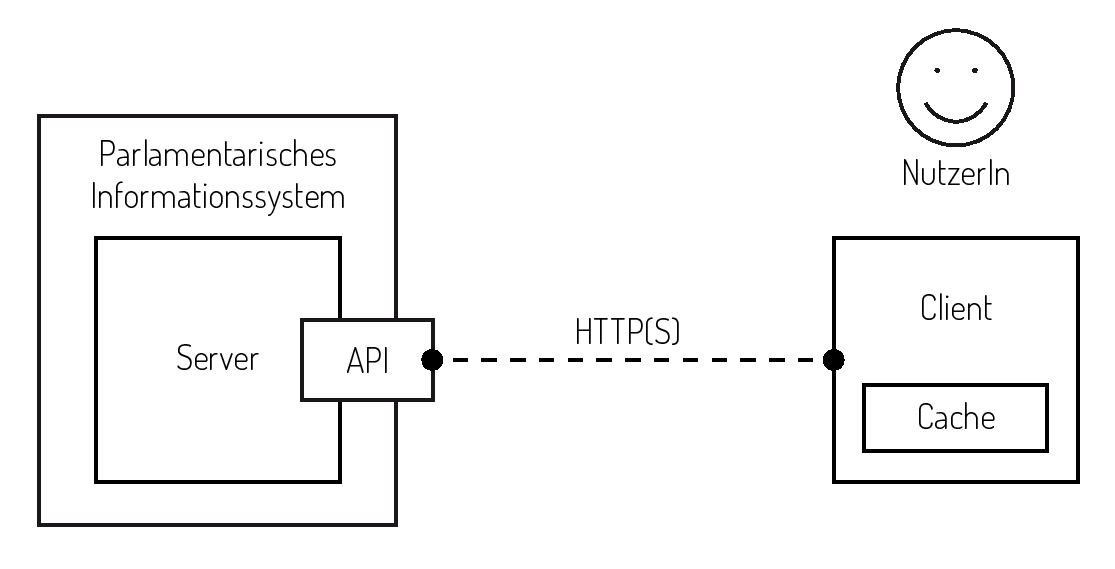
\includegraphics{images/architektur-ueberblick.png}
\caption{Architekturdiagramm}
\end{figure}

\subsection{Parlamentarisches
Informationssystem}\label{parlamentarischesux5finfosystem}

Parlamentarische Informationssysteme sind Software-Systeme, die von
verschiedensten Körperschaften eingesetzt werden, um die Zusammenarbeit
von Parlamenten zu organisieren, zu dokumentieren und öffentlich
nachvollziehbar zu machen. Zu den Körperschaften können beispielsweise
Kommunen, Landkreise, Regierungsbezirke und Zweckverbände gehören.

Diese Systeme unterstützen in der Regel mehrere der folgenden
Funktionen:

\begin{itemize}
\itemsep1pt\parskip0pt\parsep0pt
\item
  Das Erzeugen, Bearbeiten und Darstellen von Sitzungen und deren
  Tagesordnung
\item
  Das Erzeugen und Abrufen von Sitzungsprotokollen
\item
  Das Erzeugen, Bearbeiten und Anzeigen von Drucksachen
\item
  Das Erzeugen, Bearbeiten und Anzeigen von Gremien und deren
  Mitgliedern
\end{itemize}

Funktionen, die die Eingabe und Bearbeitung von Daten betreffen, sind in
der Regel einem geschlossenen Nutzerkreis vorbehalten. Die Darstellung
und der Abruf von Informationen und Dokumenten hingegen ist in vielen
Fällen für die Öffentlichkeit freigegeben.

Die OParl-Spezifikation beschreibt eine Schnittstelle, die den
maschinellen, lesenden Zugriff auf derartige Informationen ermöglicht.

\hyperdef{}{server}{\subsection{Server}\label{server}}

Der Server im Sinne dieser Spezifikation ist ein Software-Dienst, der
auf einem mit dem Internet verbundenen Rechnersystem läuft. Dieser
Dienst ist eine spezielle Form eines WWW- bzw. HTTP(S)-Servers.
Entsprechend beantwortet der Server HTTP-Anfragen, die an ihn auf einem
bestimmten TCP-Port gestellt werden.

Der Server ist als Bestandteil des parlamentarischen Informationssystems
zu verstehen. Der Betrieb des Servers steht damit üblicherweise in der
Verantwortung desjenigen, der das parlamentarischen Informationssystem
betreibt.

Von einem Server, der die OParl-Spezifikation erfüllt, wird erwartet,
dass er bestimmte parlamentarische Informationen in einem bestimmten
Format zur Verfügung stellt und auf bestimmte Anfragen von so genannten
Clients über die OParl-API entsprechend dieser Spezifikation reagiert.

\subsection{API}\label{api}

Der Begriff API steht in diesem Dokument für die
Webservice-Schnittstelle, die der Server anbietet. Die Schnittstelle
basiert auf dem HTTP-Protokoll. Mittels HTTPS ist die verschlüsselte
Nutzung der API möglich, sofern Server dies unterstützen.

Die API steht im Mittelpunkt dieser Spezifikation. Server und Clients
sind als Kommunikationspartner zu verstehen, die über das Internet als
Kommunikationskanal mit einander kommunizieren können. Die
API-Spezifikation stellt dabei die nötige Grammatik und das Vokabular
bereit, anhand dessen eine sinnvolle Kommunikation erfolgen kann.

\hyperdef{}{client}{\subsection{Client}\label{client}}

Der Begriff ``Client'' steht für eine Software, die über die OParl-API
mit dem Server kommuniziert. Da die API auf dem HTTP-Protokoll aufbaut,
handelt es sich bei dem Client um eine spezielle Form eines
HTTP-Clients.

\hyperdef{}{cache}{\subsection{Cache}\label{cache}}

Ein Cache ist ein Speicher, der einem Client dazu dienen kann, von einem
Server abgerufene Informationen längerfristig vorzuhalten. Dies kann
beispielsweise dazu dienen, mehrfache Anfragen der selben Informationen
zu vermeiden, wodurch sowohl Ressourcen auf Seite des Servers geschont
als auch die Nutzung von Netzwerkbandbreite reduziert werden kann. Die
Nutzung eines Cache kann auch zur Verbesserung der Nutzerfreundlichkeit
eines Clients beitragen, indem Wartezeiten zur Bereitstellung einer
Ressource verkürzt werden.

\subsection{Nutzerin oder Nutzer}\label{nutzerin}

Mit einer Nutzerin oder einem Nutzer ist in diesem Fall eine natürliche
Person gemeint, die mittels eines OParl-Clients auf parlamentarische
Informationen zugreift.

\subsection{Objekt}\label{objekt}

Der Server beantwortet Anfragen eines Clients im Regelfall, indem
bestimmte Objekte ausgegeben werden. Objekte sind im Fall einer
OParl-konformen API JSON-Objekte, die das Schema einhalten, das in der
vorliegenden Spezifikation beschrieben wird. Antworten des Servers
können einzelne Objekte, Listen von Objekten oder Listen von URLs von
Objekten enthalten.

\hyperdef{}{nutzungsszenarien}{\section{Nutzungsszenarien}\label{nutzungsszenarien}}

Die nachfolgenden Nutzungsszenarien dienen dazu, die Architektur und die
Anwendungsmöglichkeiten anhand konkreter Beispiele zu verdeutlichen. Sie
erheben keinen Anspruch auf Vollständigkeit.

Überblick der Szenarien:

\begin{enumerate}
\def\labelenumi{\arabic{enumi}.}
\itemsep1pt\parskip0pt\parsep0pt
\item
  Mobile Client-Anwendung
\item
  Integration in Web-Portal
\item
  Meta-Suche
\item
  Forschungsprojekt Themen- und Sprachanalyse
\end{enumerate}

\subsection{Szenario 1: Mobile
Client-Anwendung}\label{szenarioux5fmobileux5fclient}

Eine \hyperref[client]{Client}-Anwendung für mobile Endgeräte wie
Smartphones und Tablets, nachfolgend ``App'' genannt, könnte das Ziel
verfolgen, Nutzern unterwegs sowie abseits vom Desktop-PC auf die
Gegebenheiten mobiler Endgeräte optimierten Lesezugriff auf Dokumente
aus parlamentarischen Informationssystemen zu bieten. Die möglichen
Kontexte und Nutzungsmotivationen sind vielfältig:

\begin{itemize}
\item
  Teilnehmer einer Sitzung greifen während der Sitzung auf die Einladung
  dieser Sitzung und die zur Tagesordnung der Sitzung gehörenden
  Drucksachen zu, außerdem auf die Protokolle vorheriger Sitzungen.
\item
  Eine Redakteurin der Lokalpresse geht unterwegs die Themen der
  nächsten Sitzungen bestimmter Gremien, für die sie sich besonders
  interessiert, durch.
\item
  Eine Gruppe von Studierenden erkundet zusammen mit ihrem Dozenten die
  lokalpolitischen Aktivitäten des Viertels rund um ihre Hochschule.
  Dazu nutzen sie die GPS-Lokalisierung ihrer Smartphones in Verbindung
  mit den Geodaten, die an vielen Drucksachen des lokalen RIS zu finden
  sind. Direkt vor Ort an einer Baustelle öffnen sie Beschlüsse, Pläne
  und Eingaben aus dem Planfeststellungsverfahren, die dieser Baustelle
  voran gegangen sind.
\end{itemize}

Zur Realisierung derartiger Szenarien können die Fähigkeiten von
OParl-kompatiblen Servern mit den besonderen Eigenschaften der mobilen
Endgeräte verknüpft werden.

Smartphones und Tablets verfügen beispielsweise, je nach Aufenthaltsort,
über sehr unterschiedlich gute Internetanbindung. In einem Büro oder
zuhause können Nutzer über ein WLAN Daten mit hoher Bandbreite
austauschen, in Mobilfunknetzen vor allem außerhalb der Ballungsgebiete
jedoch sinken die Bandbreiten deutlich. Einige Tablets werden sogar ohne
Möglichkeit zur Mobilfunk-Datenübertragung genutzt. In solchen Fällen
kann ein \hyperref[cache]{Cache} auf dem Endgerät dazu dienen, Inhalte
vorzuhalten, die dann auch bei langsamer oder fehlender
Internetverbindung zur Verfügung stehen. Sobald dann wieder eine
Verbindung mit hoher Bandbreite bereit steht, kann die App im
Hintergrund, entweder über die \hyperref[feeds]{Feeds} der OParl API
oder über den einzelnen Abruf von Objekten, die gecachten Inhalte
aktualisieren.

Eine Stärke eines mobilen Clients ist auch die Möglichkeit der
Personalisierung, also der Anpassung auf die Bedürfnisse und Interessen
der Nutzerin oder des Nutzers. Es wäre beispielsweise denkbar, dass eine
Nutzerin die parlamentarischen Informationssysteme, für die sie sich
interessiert, dauerhaft in der App einrichtet und eine Favoritenliste
der Gremien, die ihre bevorzugten Themengebiete behandeln, hinterlegt.
Die App könnte aufgrund dieser Favoritenliste eigenständig über die API
nach neuen Sitzungsterminen, Tagesordnungspunkten, Drucksachen und
Dokumente suchen. Taucht dabei ein neues Objekt auf, wird die Nutzerin
darüber benachrichtigt. Sie kann dann beispielsweise entscheiden,
Dokumente direkt zu öffnen oder für den späteren Offline-Zugriff zu
speichern.

Einem derartigen Szenario kommt das Graph-orientierte Datenmodell der
OParl-API entgegen. Ausgehend von einer Sitzung eines bestimmten
Gremiums beispielsweise ist es damit einfach möglich, die in Verbindung
stehenden Mitglieder des Gremiums, Teilnehmer der Sitzung,
Tagesordnungspunkte der Sitzung oder Drucksachen zu den
Tagesordnungspunkten und letztlich Dokumente zu Drucksachen und Sitzung
abzurufen.

Für die Nutzer einer mobilen Client-Anwendung könnte es sich als
besonders hilfreich erweisen, wenn Dokumente auf dem Server in
verschiedenen Formaten zur Verfügung gestellt werden. Denn nicht jedes
Endgerät mit kleinem Bildschirm bietet eine nutzerfreundliche
Möglichkeit, beispielsweise Dokumente im weit verbreiteten PDF-Format
darzustellen. Hier könnte schon der Entwickler der mobilen App
Mechanismen vorsehen, die, sofern vorhanden, besser geeignete Formate
wie z. B. HTML abrufen.

Neben dem kleinen Display kann für einige mobile Endgeräte auch die im
Vergleich zu einem zeitgemäßen Desktop-PC geringere CPU-Leistung eine
Einschränkung darstellen. Solchen Geräten kommt es besonders entgegen,
wenn der Server zu allen Dokumenten auch den reinen Textinhalt abrufbar
macht, der dann beispielsweise für eine Volltextsuche auf dem Endgerät
indexiert werden kann. So wiederum kann auf dem Client eine Suchfunktion
realisiert werden, welche die OParl-API selbst nicht zur Verfügung
stellt.

Eine solche Suchfunktion kann auch über die reine Volltextsuche und über
die Suche mittels Text- oder Spracheingabe hinaus gehen. Denn ein Client
könnte von einem \hyperref[server]{Server}-System, das Drucksachen mit
Geoinformationen anbietet, diese abrufen und räumlich indexieren. Anhand
der Position des Geräts, die mittels GPS genau bestimmt werden kann,
könnte so der lokale Cache nach Objekten in der Umgebung durchsucht
werden. Das Ergebnis könnte auf einer Karte dargestellt oder in einer
Ergebnisliste angezeigt werden, die z. B. nach Distanz zum Objekt
sortiert werden kann.

\subsection{Szenario 2: Integration in
Web-Portal}\label{szenarioux5fwebux5fportal}

Portallösungen bieten den Betreibern die Möglichkeit, Inhalte auf einer
einheitlichen Weboberfläche zu veröffentlichen, die aus verschiedensten
Quellen und Plattformen bereitgestellt werden. Inhalte werden dabei
häufig als sogenannte ``Portlets'' in Seiten integriert.

Ein Beispiel für die Realisierung eines solchen Integrations-Ansatzes
wäre eine Kommune, die für ihre allgemeine Website eine Portallösung
einsetzt und hier auch Inhalte aus dem kommunalen Ratsinformationssystem
einspeisen und darstellen möchte. Die Inhalte könnten als Module mit
anderen Inhalten, beispielsweise aus einem Web Content Management System
(WCMS), gemeinsam auf einer Seite dargestellt werden.

Eine Seite über den Gemeinderat beispielsweise könnte durch ein Portlet
ergänzt werden, in dem die nächsten Sitzungstermine des Gemeinderats
aufgelistet werden. Eine Pressemeldung über ein bestimmtes Bauvorhaben,
in dem ein Beschluss erwähnt wird, könnte direkt ein Portlet mit einer
Detailansicht der entsprechenden Drucksache einbinden.

Die Portlets, die von einem Portalserver zur Verfügung gestellt werden,
stellen damit im Sinne der OParl-Architektur Clients dar. Je nach
Performanz und Anforderungen im Einzelfall könnten diese Client mit
eigenen Caches arbeiten oder aber direkt auf den jeweiligen OParl-Server
zugreifen.

Vorteil einer solchen Einbindung, also der kontextbezogenen Darstellung
von parlamentarischen Informationen im Gegensatz zu einem monolitischen
parlamentarischen Informationssystem könnte sein, dass Nutzer in einer
gewohnten und akzeptierten Oberfläche jeweils die relevanten
Informationen erhalten, ohne sich an die ungewohnte Umgebung eines
parlamentarischen Informationssystems gewöhnen zu müssen.

Die denkbaren Szenarien einer solchen Integration beschränken sich nicht
auf anonyme Nutzer von öffentlichen Websites. In einem authentifizierten
Umfeld wie beispielsweise einem kommunalen Intranet oder Extranet lassen
sich weitere Arten von Portlets und damit Mehrwerte für die Nutzer
realisieren. So könnte beispielsweise eine eingeloggte Nutzerin eine
personalisierte Liste der Sitzungstermine, zu der sie eingeladen ist,
angezeigt bekommen.

Die Standardisierung durch OParl sorgt im Rahmen der Portal-Szenarios
dazu, dass Portlets, die für ein bestimmtes parlamentarisches
Informationssystem entwickelt wurden, leichter auf andere Systeme --
auch verschiedener Anbieter -- ausgeweitet werden können, sofern diese
ebenfalls OParl-konform sind. Dies ermöglicht es beispielsweise
verschiedenen Kommunen, bei der Entwicklung von Portlets
zusammenzuarbeiten und ihre Ergebnisse auszutauschen. Denkbar sind auch
Portlet-Entwicklungen als Open-Source-Projekte.

\subsection{Szenario 3: Meta-Suche}\label{szenarioux5fmetaux5fsuche}

Die Ermöglichung einer nutzerfreundlichen Suche, die damit verbundene
Indexierung von verschiedensten Dokumenteninhalten und die
Kategorisierung von Inhalten kann eine sowohl konzeptionell als auch
technisch anspruchsvolle Aufgabe sein. Auch im Hinblick auf die
Server-Ressourcen sind damit nennenswerte Aufwände verbunden.
Andererseits liegt auf der Hand, dass die effiziente Arbeit mit großen
Informationsmengen nach intelligenten Möglichkeiten der Einschränkung
von Informationsmengen auf jeweils im Anwendungsfall relevante Treffer
verlangt. Beispiel wäre ein Nutzer, der sich für alle Dokumente zum
Thema Kreisverkehre interessiert. Die OParl-Spezifikation sieht keine
Methoden vor, wie die Ausgabe des Servers schon bei der Anfrage von
Dokumenten derart beschränkt werden können. Damit ist die Realisation
von Such- und Filtermechanismen im OParl-Umfeld eine Aufgabe, die bis
auf weiteres lediglich auf Seite der Clients angeboten werden kann.

Angelehnt an das seit den Anfängen des Webs etablierte Modell der
externen Web-Suchmaschine sind spezielle Suchmaschinen für
OParl-konforme parlamentarische Informationssysteme denkbar. Diese
können auch von dritten, beispielsweise zivilgesellschaftlichen
Organisationen betrieben werden, die nicht Betreiber des Server-Systems
sind. Solche Plattformen treten gegenüber dem OParl-Server als Client
auf und rufen bestimmte oder sämtliche Informationen, die das System
bereit hält, ab. Vorbild sind die Robots oder Spider von
Web-Suchmaschinen. Die abgerufenen Informationen können dann indexiert
und je nach Anforderungen für eine gezielte Suche weiterverarbeitet
werden.

Dieses Modell ist grundsätzlich nicht auf einzelne OParl-Server oder
einzelne Körperschaften beschränkt. Vielmehr könnte der Betreiber einer
solchen Suchmaschine sich entschließen, die Informationen aus mehreren
OParl-konformen Systemen zu indexieren. Nutzern könnte entweder
angeboten werden, die Suche auf bestimmte Körperschaften, beispielsweise
auf eine bestimmte Kommune, zu beschränken, oder ohne Beschränkung über
alle angebotenen Körperschaften zu suchen.\footnote{Daher der Begriff
  Meta-Suche}

Daraus ergeben sich vielfältige Anwendungsszenarien, die hier
beispielhaft beschrieben werden:

\begin{itemize}
\item
  Eine Mitarbeiterin eines regionalen Zweckverbands hat die Aufgabe,
  Ratsvorgänge in den Mitgliedskommunen mit Relevanz für die Aufgaben
  des Verbandes im Blick zu behalten. Sie nutzt dafür ein regionales
  Internetportal, in dem die Inhalte der OParl-konformen
  parlamentarischen Informationssysteme der Mitgliedskommunen
  durchsuchbar sind. Um die Suche zu vereinfachen, hat sie einzelne
  Schlagwörter abonniert, zu denen sie automatisch über neue Vorgänge
  informiert wird.
\item
  Ein Einwohner eines Ballungsraums will sich über aktuelle Vorgänge
  rund um seine Mietwohnung in Stadt A, sein Gartengrundstück in einer
  Kleingartenkolonie in der Nachbarstadt B und seinen Arbeitsplatz in
  Stadt C auf dem Laufenden halten. Dazu abonniert er im regionalen
  Meta-Such-Portal parlamentarische Vorgänge mit räumlichem Bezug zu
  diesen drei Standorten und wird so automatisch über neue Aktivitäten
  informiert, die Relevanz für ihn haben könnten.
\item
  Eine Landespolitikerin möchte einfacher über die politischen
  Aktivitäten ihrer Parteikollegen in den Rathäusern des Bundeslandes
  informiert werden. Dazu nutzt sie ein Internetportal, in dem die
  Informationen aus den parlamentarischen Informationssystemen mit
  OParl-Schnittstelle im Land zusammengeführt werden. Dort hat sie sich
  Abonnements zu einzelnen Lokalpolitikern eingerichtet und wird
  automatisch über ihre Teilnahme an Gremiensitzungen und die Themen
  dieser Sitzungen informiert.
\end{itemize}

\subsection{Szenario 4: Forschungsprojekt Themen- und
Sprachanalyse}\label{szenarioux5fforschung}

In einem Forschungsprojekt sollen Pro- und Contra-Argumentationen bei
Ratsdiskussionen zum Ausbau von Stromtrassen identifiziert werden. Über
die Analyse in mehreren Gebietskörperschaften sollen die gefundenen
Argumentationen zu wiederkehrenden Mustern verdichtet werden und
festgestellt werden, wie diese Muster regional abweichen.

Dazu nutzen die Mitarbeitenden des Forschungsprojektes die
OParl-Schnittstellen der parlamentarischen Informationssysteme aller
Kommunen entlang der geplanten überregionalen Trassen. Über diese
einheitlichen Schnittstellen können sie insbesondere die relevanten
Wortprotokolle abrufen und zum Beispiel in einem Werkzeug zur
qualitativen Datenanalyse lokal verarbeiten. Im Ergebnis ließe sich auch
erkennen, wie ähnlich oder wie unterschiedlich die Argumente in
rhetorischer Hinsicht vorgetragen werden.

\section{Prinzipien und Funktionen des
Schnittstelle}\label{prinzipien-und-funktionen-des-schnittstelle}

In diesem Kapitel werden grundlegende Funktionsprinzipien einer
OParl-Schnittstelle beschrieben.

\hyperdef{}{designprinzipien}{\subsection{Designprinzipien}\label{designprinzipien}}

\subsubsection{Aufbauen auf gängiger
Praxis}\label{aufbauen-auf-guxe4ngiger-praxis}

Grundlage für die Erarbeitung der OParl-Spezifikation in der
vorliegenden Version ist eine Analyse von aktuell (2012 bis 2014) in
Deutschland etablierten parlamentarischen Informationssystemen und ihrer
Nutzung. Erklärtes Ziel für diese erste Version ist es, mit möglichst
geringem Entwicklungsaufwand auf Seite der Softwareanbieter und
Migrationsaufwand auf Seite der Betreiber zu einer Bereitstellung von
parlamentarischen Informationen über eine OParl-API zu gelangen. Hierbei
war es von entscheidender Bedeutung, dass sich die Informationsmodelle
der einschlägigen Softwareprodukte stark ähneln. Für die
OParl-Spezifikation wurde sozusagen ein Datenmodell als ``gemeinsamer
Nenner'' auf Basis der gängigen Praxis beschrieben.

\subsubsection{Verbesserung gegenüber dem Status Quo wo
möglich}\label{verbesserung-gegenuxfcber-dem-status-quo-wo-muxf6glich}

Dort, wo es dem Ziel der einfachen Implementierbarkeit und der einfachen
Migration nicht im Weg steht, erlauben sich die Autoren dieser
Spezifikation, auch Funktionen aufzunehmen, die noch nicht als gängige
Praxis im Bereich der Ratsinformationssysteme bezeichnet werden können
oder welche nur von einzelnen Systemen unterstützt werden. Solche
Funktionen sind dann so integriert, dass sie nicht als zwingende
Anforderung gelten.

Ein Beispiel für eine derartige Funktion ist die Abbildung von Geodaten
im Kontext von Drucksachen (\texttt{oparl:Paper}), um beispielsweise die
Lage eines Bauvorhabens, das in einer Beschlussvorlage behandelt wird,
zu beschreiben. Zwar ist den Autoren nur ein einziges parlamentarisches
Informationssystem\footnote{Das Ratsinformationssystem BoRis, eine
  Eigenentwicklung der Stadt Bonn
  \url{http://www2.bonn.de/bo_ris/ris_sql/agm_index.asp}} in Deutschland
bekannt, das Geoinformationen -- und zwar in Form von Punktdaten, also
einer Kombination aus Längen- und Breitengradangaben -- mit Dokumenten
verknüpft. Der Vorteil dieser Funktion ist jedoch anhand zahlreicher
Anwendungsszenarien belegbar. Somit ist der vorliegenden
OParl-Spezifikation die Möglichkeit beschrieben, Geodaten-Objekte
einzubetten.

Die Angabe eines einzelnen Punktes ist dabei nur ein einfacher
Sonderfall. Die Spezifikation erlaubt auch die Kodierung von mehreren
Objekten, die Punkte, Linien oder Polygone repräsentieren können. Vgl.
dazu \texttt{oparl:Location}.

Auch die Ausgabe einer Nur-Text-Version im Kontext des Dokuments
(\texttt{oparl:File}), das den barrierefreien Zugriff auf Inhalte oder
Indexierung für Volltextsuchfunktionen deutlich vereinfacht, ist eine
Möglichkeit, die in der gängigen Praxis noch nicht zu finden ist. Ebenso
die Möglichkeit, Beziehungen zwischen einzelnen Dokumenten herzustellen,
um so von einem Dokument zu anderen Dokumenten mit identischem Inhalt,
aber in anderen technischen Formaten zu verweisen, etwa von einer
ODT-Datei zu einer PDF-Version.

\hyperdef{}{restful}{\subsubsection{RESTful}\label{restful}}

Die Bezeichnung ``REST'' (für ``Representational State Transfer'') wurde
im Jahr 2000 von Roy Fielding eingeführt\footnote{Fielding, Roy:
  Architectural Styles and the Design of Network-based Software
  Architectures,
  \url{http://www.ics.uci.edu/~fielding/pubs/dissertation/top.htm}}. Die
Definition von Fielding reicht sehr weit und berührt viele Details. In
der Praxis wird der Begriff häufig genutzt, um eine Schnittstelle zu
beschreiben,

\begin{itemize}
\itemsep1pt\parskip0pt\parsep0pt
\item
  die auf WWW-Technologie aufbaut, insbesondere dem HTTP-Protokoll
\item
  die darauf beruht, dass mittels URL einzelne Ressourcen oder Zustände
  vom Client abgerufen werden können.
\item
  die zustandslos ist. Das bedeutet, die Anfrage eines Clients an den
  Server enthält alle Informationen, die notwendig sind, um die Anfrage
  zu verarbeiten. Auf dem Server wird kein Speicher zur Verfügung
  gestellt, um beispielsweise den Zustand einer Session zu speichern.
\end{itemize}

Diese Prinzipien macht sich auch OParl zunutze. Damit gilt prinzipiell,
dass eine OParl-konforme Server-Schnittstelle auch als ``RESTful''
gelten darf.

\subsubsection{Selbstbeschreibungsfähigkeit}\label{selbstbeschreibungsfuxe4higkeit}

Ausgaben des Servers sollten so beschaffen sein, dass sie für
menschliche Nutzerinnen weitgehend selbsterklärend sein können. Dies
betrifft besonders die Benennung von Objekten und Objekteigenschaften.

Aber auch für die maschinelle Verarbeitung der Daten durch Clients kann
die Selbstbeschreibung wichtig sein. Dies stellt allerdings erhöhte
Anforderungen an die verwendeten Datenformate, da dafür formalisierte
semantische Informationen enthalten sein müssen.

Um den Kreis der Entwicklerinnen und Entwickler, die mit einer OParl-API
arbeiten können, nicht unnötig einzuschränken, wird hierbei
grundsätzlich auf englischsprachige Begrifflichkeiten gesetzt.

\hyperdef{}{erweiterbarkeit}{\subsubsection{Erweiterbarkeit}\label{erweiterbarkeit}}

Implementierer sollen in der Lage sein, über eine OParl-konforme
Schnittstelle auch solche Informationen auszugeben, die nicht im Rahmen
des OParl-Schemas abgebildet werden können. Dies bedeutet zum einen,
dass ein System Objekttypen unterstützen und ausliefern darf, die nicht
(oder noch nicht) im OParl-Schema beschrieben sind. Das bedeutet auch,
dass Objekttypen so um eigene Eigenschaften erweitert werden können, die
nicht im OParl Schema beschrieben sind.

Ein weiterer Aspekt betrifft die Abwärtskompatibilität, also die
Kompatibilität von OParl-Clients mit zukünftigen Schnittstellen. So
können beispielsweise zukünftige Erweiterungen des OParl-Schemas, etwa
um neue Objekttypen, genau so durchgeführt werden, wie die Erweiterungen
um herstellerspezifische Objekttypen. Ein Client muss diese Anteile
nicht auswerten, sofern sie nicht für die Aufgabe des Clients relevant
sind.

\subsubsection{Browseability/Verlinkung}\label{browseabilityux5fverlinkung}

Klassische Webservice-Schnittstellen erfordern von den Entwicklern
vollständige Kenntnis der angebotenen Einstiegspunkte und
Zugriffsmethoden, gepaart mit sämtlichen unterstützten URL-Parametern,
um den vollen Funktionsumfang der Schnittstelle ausschöpfen zu können.

Parlamentarische Informationen sind weitgehend in Form von Graphen
aufgebaut. Das bedeutet, dass Objekte häufig mit einer Vielzahl anderer
Objekte verknüpft sind. So ist eine Person beispielsweise Mitglied in
mehreren Gremien, das Gremium hat mehrere Sitzungen abgehalten und zu
diesen Sitzungen gibt es jeweils zahlreiche Drucksachen, die ihrerseits
wieder zahlreiche Dokumente enthalten.

Eine OParl-Schnittstelle gibt jedem einzelnen Objekt eine eindeutige
Adresse, eine URL. Somit kann die Schnittstelle den Verweis von einem
Objekt, beispielsweise einem Gremium, auf ein anderes Objekt, etwa ein
Mitglied des Gremiums, dadurch ausgeben, dass im Kontext des Gremiums
die URL des Mitglieds ausgeben wird. Der Client kann somit ausgehend von
einem bestimmten Objekt die anderen Objekte im System finden, indem er
einfach den angebotenen URLs folgt. Dieses Prinzip wird auch ``Follow
Your Nose''\footnote{\url{http://patterns.dataincubator.org/book/follow-your-nose.html}}
genannt.

\subsubsection{Linked Data}\label{linkedux5fdata}

Der Begriff ``Linked Data'' steht für die Beschreibung von Daten in
einer Form, die diese über ihren ursprünglichen Kontext hinaus
verständlich macht.\footnote{vgl. Bundesministerium des Innern
  (Herausg.): Open Government Data Deutschland, Seite 433f., 2012
  \url{http://www.bmi.bund.de/SharedDocs/Downloads/DE/Themen/OED_Verwaltung/ModerneVerwaltung/opengovernment.pdf}}

Kern von Linked Data ist die Möglichkeit, alle Bestandteile von Daten in
Form von Tripeln zu beschreiben, das sind dreiteilige
Informationseinheiten aus einem Subjekt, einem Prädikat und einem
Objekt. Alle drei Bestandteile können in Form global eindeutiger
``Uniform Resource Identifier'' (URI) abgebildet werden.

Nach dem Linked-Data-Prinzip könnte beispielsweise der Vorname einer
Person mit dem folgenden Tripel beschrieben werden:

\begin{itemize}
\itemsep1pt\parskip0pt\parsep0pt
\item
  \textbf{Subjekt}: http://dbpedia.org/resource/John\_Doe\_(musician)
\item
  \textbf{Prädikat}: http://xmlns.com/foaf/0.1/givenName
\item
  \textbf{Objekt}: http://dbpedia.org/resource/John\_(given\_name)
\end{itemize}

Hierbei macht man von der Tatsache Gebrauch, dass das Subjekt, also die
Person, um die es geht, bereits mittels ihrer URI eindeutig
identifiziert werden kann, und dass bestenfalls unter dieser URI weitere
Informationen zu der Person abrufbar sind.\footnote{Ein Aufruf der URL
  \url{http://dbpedia.org/resource/John_Doe_(musician)} im herkömmlichen
  Web-Browser führt zu einer Weiterleitung auf die URL
  \url{http://dbpedia.org/page/John_Doe_(musician)}. Siehe dazu auch der
  Abschnitt \hyperref[contentux5fnegotiation]{Content Negotiation}} Auch
für das Prädikat ``Person hat den Vornamen'' liegt bereits eine
Beschreibung in einem gebräuchlichen Vokabular vor, auf das hier
verwiesen werden kann. Und schließlich kann sogar der eigentliche
Vorname in Form einer URI abgebildet werden, nämlich als Verweis auf
eine umfangreiche Beschreibung dieses Namens.

Das \textbf{Ziel} von OParl ist es, mit der vorliegenden Version 1.0 der
Spezifikation, die Nutzung solcher allgemeingültigen Vokabulare für die
Veröffentlichung von parlamentarischen Informationen zu begünstigen und
die automatisierte Verarbeitung und Verknüpfung von Informationen, auch
über die Grenzen verschiedener Informationssysteme hinweg, zu
erleichtern.

Beispiele, wo dies sinnvoll ist, sind in der Praxis leicht zu finden. So
finden sich beispielsweise in vielen lokalen Parlamenten immer wieder
Fraktionen der selben Parteien, beispielsweise CDU und SPD. Mittels
Linked Data wäre es möglich, jede dieser Fraktionen mit einer externen
URL zu verknüpfen\footnote{beispielsweise
  \url{http://dbpedia.org/resource/Christian_Democratic_Union_(Germany)}
  und
  \url{http://dbpedia.org/resource/Social_Democratic_Party_of_Germany}}
und somit erkennbar zu machen, zu welcher Partei diese Fraktion gehört.
Ebenso finden sich viele inhaltliche Ähnlichkeiten bei Gremien wie zum
Beispiel Ausschüssen (z. B. Hauptausschuss, Verkehrsausschuss etc.) oder
bei Arten von Drucksachen (z. B. Anträge, Anfragen, Mitteilungen,
Beschlussvorlagen).

Mit der Möglichkeit, Objekte mit Hilfe von URLs zu klassifizieren (vgl.
\hyperref[vokabulareux5fklassifizierung]{Vokabulare zur
Klassifizierung}), geht diese Version von OParl einen ersten Schritt in
Richtung Linked Data. Die Aufgabe, ein übergreifend nutzbares Vokabular
anhand von Anforderungen aus der Praxis zu erstellen, kann damit als
logischer nächster Schritt in naher Zukunft angegangen werden.

\subsubsection{Kriterien für die Aufnahme von Klassen und
Eigenschaften}\label{kriterien-fuxfcr-die-aufnahme-von-klassen-und-eigenschaften}

Bei der Erstellung des Vokabulars (Klassen und Eigenschaften) gab es
viel Input von mehreren RIS-Herstellern und Anwendern der berücksichtigt
werden musste.

Dies ist eine keineswegs abschliessende Liste von Kriterien die dabei
eine Rolle gespielt haben:

\begin{itemize}
\itemsep1pt\parskip0pt\parsep0pt
\item
  Erforderlichkeit für Formulierung relevanter Informationen
\item
  Verständlichkeit der Semantik
\item
  Vermeidung von Redundanzen
\item
  Kompatibilität mit anderen Vokabularen und Spezifikationen
\item
  Konsistenz der Benennung
\item
  Konsistenz verwendeter Mechanismen
\item
  Speicherbedarf auf Client-Seite (Cache)
\item
  benötigte Netz-Bandbreite
\item
  Anzahl http-Requests bis Client alle benötigten Daten hat
\end{itemize}

Diese Kriterien können je nach Einsatzszenario von sehr
unterschiedlichem Gewicht sein und sich widersprechen. Bei den
Entscheidungen mussten deshalb regelmäßig Abwägungen vorgenommen werden
und auch neue Lösungen entwickelt werden, die so bisher in keinem RIS
umgesetzt sind - aber nach Überzeugung der Autoren mit akzeptablem
Aufwand umsetzbar sind.

Bei der Erstellung der Spezifikation wurde auch versucht, Dokumente des
W3C zur Erstellung hochwertiger Spezifikationen\footnote{QA Framework:
  Specification Guidelines: \url{http://www.w3.org/TR/qaframe-spec/},
  W3C Manual of Style: \url{http://www.w3.org/2001/06/manual/}} zu
berücksichtigen.

\subsection{Zukunftssicherheit}\label{zukunftssicherheit}

Wie unter \hyperref[designprinzipien]{Designprinzipien} beschrieben, ist
diese erste Version der OParl-Spezifikation bereits im Wesentlichen von
den Zielen der einfachen Implementierbarkeit und Migration geleitet.

Der Aufwand, den die Betreiber von parlamentarischen
Informationssystemen bei der Bereitstellung von OParl-konformen
Schnittstellen betreiben, soll auch bei der zukünftigen
Weiterentwicklung dieser Spezifikation berücksichtigt werden. Ebenso
soll den Entwicklern von Client-Software zukünftig entgegen kommen, dass
ihre bestehenden Clients auch mit Servern kommunizieren können, die eine
neuere Version der OParl-Spezifikation unterstützen. Dieser Wunsch ist
bereits im Designprinzip \hyperref[erweiterbarkeit]{Erweiterbarkeit}
ausformuliert.

Mit anderen Worten: die Autoren der OParl-Spezifikation beabsichtigen
größtmögliche Zukunftssicherheit und zukünftige Abwärtskompatibilität.
Dieses Ziel wird in Zukunft natürlich abgewägt werden müssen mit dem
Wunsch, sich an Veränderungen und neue Erkenntnisse anzupassen. Eine
Garantie für Zukunftssicherheit kann insofern niemand aussprechen.

Ein fiktives Szenario soll verdeutlichen, dass es zweckmäßig ist, schon
beim Betrieb eines OParl 1.0 Servers die zukünftige Entwicklung im Blick
zu haben:

\begin{itemize}
\item
  Die Kommune \emph{Beispielstadt} betreibt ihren OParl-1.0-Server unter
  der URL \texttt{https://oparl.example.org/1.0/}.
\item
  Verschiedene Clients, die für OParl Version 1.0 entwickelt wurden,
  kommen bei Nutzerinnen und Nutzern, die sich für den Stadtrat in
  Beispielstadt intressieren, zum Einsatz. Jeder Client-Nutzer hat dazu
  lediglich die URL \texttt{https://oparl.example.org/1.0/} des
  OParl-Servers in der Client-Konfiguration hinterlegt.
\item
  Die OParl-Spezifikation wird aktualisiert, es erscheint Version 1.1.
  Das Schema enthält Erweiterungen gegenüber Version 1.0, jedes gültige
  Objekt aus Version 1.0 behält jedoch auch weiterhin seine Gültigkeit.
  Und Objekte, die nach Version 1.1 gültig sind, sind auch für Clients
  gültig, die für Version 1.0 entwickelt wurden.
\item
  Die Firma, die den OParl-Server von Beispielstadt entwickelt hat,
  liefert ein Update.
\item
  Der OParl-Server von Beispielstadt ist nun über eine neue URL
  \texttt{https://oparl.example.org/1.1/} zu erreichen. Alle Anfragen an
  \texttt{https://oparl.example.org/1.0/...} werden auf die
  entsprechende URL unter \texttt{https://oparl.example.org/1.1/} mit
  HTTP-Redirects und Status-Code 301 weiter geleitet.
\item
  Die Nutzer der Clients, die mit dem OParl-Server von Beispielstadt
  arbeiten, können weiter arbeiten wie bisher. Sie erhalten vom Client
  höchstens einmalig eine Information, dass sich die Server-URL geändert
  hat.
\item
  Einzelne Client-Nutzerinnen werden von den Anbietern ihrer Clients
  darauf aufmerksam gemacht, dass eine neue Version ihres Produkts für
  eine neue OParl-Version zur Verfügung steht. Mit dieser Version
  könnten die Nutzer in den Genuss der Vorteile von OParl-Version 1.1
  kommen.
\item
  Nach einiger Zeit erscheint eine neue Version 2.0 der
  OParl-Spezifikation. Hier haben sich größere Änderungen ergeben. Das
  Schema ist nicht kompatibel mit dem von Version 1.0 und 1.1. Clients,
  die für eine Version 1.* entwickelt wurden, werden nicht sinnvoll mit
  einem Server der Version 2 kommunizieren können.
\item
  Der Server-Entwickler bietet das entsprechende Produkt zu
  OParl-Version 2 an, Beispielstadt entschließt sich zum Einsatz der
  neuen Version. Da das Server-Produkt gleichzeitig OParl 1.* und OParl
  2.0 bedienen kann, kann Beispielstadt gleichzeitig einen Endpunkt für
  1.1 und einen für 2.0 betreiben. Die URL des neuen Endpunkts lautet
  \texttt{https://oparl.example.org/2.0/}.
\end{itemize}

Das Szenario verdeutlicht, wie insbesondere zwei Aspekte für eine
möglichst sanfte Migration zwischen den OParl-Versionen sorgen können:

\begin{enumerate}
\def\labelenumi{\arabic{enumi}.}
\item
  Dedizierte API-Endpunkt-URLs für jede OParl-Version
\item
  HTTP-Weiterleitungen auf die neue URL, sofern diese kompatibel mit der
  alten ist, erspart den Parallelbetrieb von zwei ähnlichen Endpunkten
  und kommuniziert den Clients automatisch den Endpunkt der neuen
  Version
\end{enumerate}

Zu der Art, wie die OParl-Version sich auf die Endpunkt-URL auswirkt,
will diese Spezifikation keine Vorgaben machen. Die Pfad-Elemente im
obigen Szenario sind Vorschläge, aber in keiner Weise bindend.

Die praktische Umsetzung von HTTP-Weiterleitungen ist besonders dann
einfach, wenn die restlichen URL-Bestandteile identisch bleiben. In
diesem Fall können Server mit einer einfachen Regel von jeglicher
vorherigen auf jegliche neue URL weiterleiten.

\hyperdef{}{http-und-https}{\subsection{HTTP und
HTTPS}\label{http-und-https}}

OParl-Server und -Client kommunizieren miteinander über das
HTTP-Protokoll.

Hierbei SOLL eine verschlüsselte Variante des Protokolls, HTTPS, zum
Einsatz kommen. Dabei werden auch die URLs verschlüsselt, deren Kenntnis
möglicherweise Rückschlüsse auf Interessen von Nutzer ermöglicht.
Alternativ kann jedoch auch unverschlüsseltes HTTP verwendet werden.
Welche Verschlüsselungstechnologie im Fall von HTTPS gewählt wird,
obliegt dem Betreiber bzw. Server-Implementierer.

Die Wahl des unverschlüsselten oder verschlüsselten HTTP-Zugriffs hat
Auswirkung auf die im System verwendeten URLs. Wie im Kapitel
\hyperref[urls]{URLs} beschrieben, verfolgt diese Spezifikation die
Festlegung auf genau eine ``kanonische'' URL je Ressource (vgl.
\hyperref[urlux5fkanonisierung]{URL-Kanonisierung}).

Bei unverschlüsseltem Zugriff wird allen URLs, die auf das betreffende
System zeigen, das Schema ``http://'' voran gestellt, beim
verschlüsselten Zugriff stattdessen ``https://''.

Es ist daher ZWINGEND, dass der Server-Betreiber sich zur
URL-Kanonisierung für nur eine von beiden Varianten entscheidet.
Beantwortet das System regulär Anfragen über HTTPS mit der Auslieferung
von Objekten etc., dann gilt für Anfragen an die entsprechende
unverschlüsselte URL ZWINGEND:

\begin{itemize}
\item
  unter der URL ist kein Webserver erreichbar, oder
\item
  der Server unter der URL beantwortet die Anfrage mit einer
  Weiterleitung an die HTTPS-URL (HTTP Status-Code 301)
\end{itemize}

Gleiches gilt umgekehrt: hat sich der Betreiber generell für den Betrieb
des OParl-Servers über unverschlüsseltes HTTP entscheiden, dann MUSS für
die entsprechenden HTTPS-URLs eine der beiden folgenden Möglichkeiten
gelten:

\begin{itemize}
\item
  Entweder ist unter den entsprechenden HTTPS-URLs kein Webserver
  erreichbar
\item
  oder Anfragen an die HTTPS-URLs werden mit Redirects auf die
  entsprechenden HTTP-URLs beantwortet (FRAGE: ist das ein sinnvolles
  Szenario?).
\end{itemize}

\hyperdef{}{urls}{\subsection{URLs, IRIs und URIs}\label{urls}}

Den URLs (für \emph{Uniform Resource Locators}) kommt bei einer
OParl-konformen API eine besondere Bedeutung zu und es werden eine Reihe
von Anforderungen an die Verarbeitung von URLs gestellt.

Im Rahmen dieses Dokuments wird aus Gründen der Verständlichkeit
generell der allgemein gebräuchliche Begriff \emph{URL} werwendet, auch
wenn damit tatsächlich die internationalisierte Variante nach RFC
3987\footnote{RFC 3987: \url{http://tools.ietf.org/html/rfc3987}}, die
korrekterweise \emph{IRI} bzw. \emph{Internationalized Resource
Identifier} genannt werden müsste, gemeint ist. Einige Quellen wiederum
nutzen den Begriff \emph{URI} bzw. \emph{Uniform Resource Identifier}.
Das vorliegende Dokumente fasst alle drei Konzepte mit dem Begriff
\emph{URL} zusammen und ignoriert damit die Unterschiede der einzelnen
Begriffe, da diese im Rahmen dieser Spezifikation nicht von Bedeutung
sind.

Die grundsätzliche Funktionsweise von URLs ist in RFC 3986
beschrieben\footnote{RFC 3986: \url{http://tools.ietf.org/html/rfc3986}}.
Darauf aufbauend sind hier die Bestandteile einer beispielhaften URL mit
den Bezeichnungen beschriftet, mit denen sie in diesem Dokument benannt
werden:

\begin{figure}[htbp]
\centering
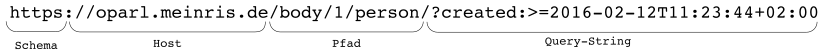
\includegraphics{images/url.png}
\caption{Benennung von URL-Bestandteilen}
\end{figure}

Der optionale \emph{Query-String} besteht dabei aus beliebig vielen
\emph{Query-Parametern}, die jeweils einen Namen (links des
Gleichheitszeichens) und einen Wert haben können.

\hyperdef{}{urlux5fkanonisierung}{\subsubsection{URL-Kanonisierung}\label{urlux5fkanonisierung}}

Absicht ist, dass jedes Objekt, das ein Server über eine OParl-API
anbietet, über genau eine URL identifizierbar und abrufbar ist. Diese
Vereinheitlichung der URL wird nachfolgend \emph{Kanonisierung} genannt.

Die Kanonisierung ist entscheidend, um erkennen zu können, ob zwei URLs
das selbe Objekt repräsentieren. Sind zwei URLs identisch, sollen
Clients daraus ableiten können, dass diese das selbe Objekt
repräsentieren. Sind zwei URLs unterschiedlich, soll im Umkehrschluss
die Annahme gelten, dass sie zwei verschiedene Objekte repräsentieren.

Der OParl-konforme Server MUSS für jedes benannte Objekt eine kanonische
URL bestimmen können.

Die URL-Kanonisierung betrifft sämtliche Bestandteile der URL.
Entsprechend beginnt diese schon beim \textbf{Schema} und bei der
Entscheidung durch den Betreiber, ob eine OParl-API regulär über HTTP
oder über HTTPS erreichbar sein soll (vgl.
\hyperref[http-und-https]{HTTP und HTTPS}).

Der \textbf{Host}-Teil der URL wird ebenfalls durch die Konfiguration
des Betreibers festgelegt. Obwohl technisch auch die Verwendung einer
IP-Adresse (z.B. ``123.123.123.123'') möglich wäre, SOLL der Betreiber
einen mit Bedacht gewählten Host-Namen einsetzen. Die Vorteile dieser
Lösung gegenüber der Verwendung einer IP-Adresse sind vielfältig:

\begin{itemize}
\itemsep1pt\parskip0pt\parsep0pt
\item
  Nutzerinnen können Host-Namen lesen und interpretieren
\item
  In Kombination mit der richtigen Domain (oder Subdomain) kann der
  Hostname kommunizieren, wer der Betreiber ist.
\item
  Host-Namen können zwischen verschiedenen technischen Systemen (bzw.
  von IP-Adresse zu IP-Adresse) migriert werden, was hilft, die
  Langlebigkeit der URLs zu gewährleisten
\end{itemize}

Eine URL wie

\begin{verbatim}
http://oparl.stadtrat.stadt-koeln.de/
\end{verbatim}

kommuniziert beispielsweise direkt die Zugehörigkeit zur Stadt Köln als
Betreiber des Systems. Die Bezeichnung ``stadtrat'' in der Subdomain
zeigt den Zweck des Systems allgemein verständlich an. Der Host-Name
``oparl.stadtrat.stadt-koeln.de'' deutet an, dass diese URL zu einer
OParl-Schnittstelle zu diesem System gehört. Eine technische
Notwendigkeit zur Verwendung einer eigenen Domain für OParl besteht
jedoch nicht, da JSON-Dokumente und HTML-Seiten mittels Content
Negotiation über eine gemeinsame Domain ausgeliefert werden können.

Um die Kanonisierung zu gewährleisten, SOLLEN Betreiber alle
Möglichkeiten ausschließen, die dazu führen können, dass eine Ressource
neben der kanonischen URL noch über andere URLs abrufbar ist. Diese
Faktoren können sein:

\begin{itemize}
\item
  Der selbe Server antwortet nicht nur über den kanonischen Host-Namen,
  sondern auch noch über andere Host-Namen. Das könnte zum Beispiel der
  Fall sein, wenn der Host-Name als CNAME für einen anderen Namen
  konfiguriert wurde oder wenn ein DNS A-Record für die IP-Adresse des
  Servers existiert.
\item
  Der Server ist neben dem Host-Namen auch über die IP-Adresse
  erreichbar.
\item
  Zusätzliche Domains, die einen A-Record auf den selben Server besitzen
\end{itemize}

Zu der kanonischen Beispiel-URL https://oparl.stadtrat.stadt-koeln.de/
wären eine Reihe von nicht-kanonischen URL-Varianten denkbar, die
technischen auf den selben Server führen könnten:

\begin{itemize}
\itemsep1pt\parskip0pt\parsep0pt
\item
  https://83.123.89.102/
\item
  https://oparl.stadtrat.stadtkoeln.de/
\item
  https://risserv.stadt-koeln.de/
\end{itemize}

Falls es aus technischen Gründen nicht möglich ist, den Zugang auf das
OParl-System über nicht-kanonische URLs zu unterbinden, SOLL eine
entsprechende HTTP-Anfrage mit einer Weiterleitung auf die entsprechende
kanonische URL beantwortet werden. Dabei ist der HTTP-Status-Code 301 zu
verwenden.

Server-Implementierern wird empfohlen, hierfür den \texttt{Host}-Header
der HTTP-Anfrage auszuwerten und mit der konfigurierten Einstellung für
den kanonischen Host-Namen des Systems abzugleichen.

Beim \textbf{Pfad}-Bestandteil der URL MÜSSEN Server-Implementierer
darüber hinaus beachten, dass nur jeweils eine Schreibweise als die
kanonische Schreibweise gelten kann. Dazu gehört auch die Groß- und
Kleinschreibung, die Anzahl von Schrägstrichen als Pfad-Trennzeichen,
die Anzahl von führenden Nullen vor numerischen URL-Bestandteilen und
vieles mehr.

Die Kanonisierung umfasst auch den \textbf{Query-String}-Bestandteil der
URL. Wie auch beim Pfad, gilt hier, dass für jeden Parameter und jeden
Wert im Query-String nur eine kanonische Schreibweise gelten MUSS.

Darüber hinaus SOLL der Server-Implementierer darauf achten, bei
Verwendung von Query-String-Parametern diese in URLs immer nach dem
selben Prinzip zu sortieren. Ein Beispiel: die beiden URLs

\begin{verbatim}
https://oparl.example.org/members?body=1&committee=2
https://oparl.example.org/members?committee=2&body=1
\end{verbatim}

unterscheiden sich lediglich in der Reihenfolge der
Query-String-Parameter. Da sie jedoch nicht identisch sind, müssen
Clients annehmen, dass beide URLs verschiedene Objekte repräsentieren.
In der Konsequenz kann es zu vermeidbarer Ressourcennutzung sowohl auf
Client- als auch auf Serverseite kommen.

Von Clients wird erwartet, dass sie die URLs, die ihnen von Servern
angeboten werden, unverändert verwenden. Clients SOLLEN NICHT versuchen,
Schreibweisen von URLs zu ändern, Query-String-Parameter umzusortieren
oder Ähnliches.

\subsubsection{Langlebigkeit}\label{langlebigkeit}

Weiterhin ist es Absicht, dass URLs von Objekten langlebig sind, so dass
sie, wenn sie einmal verbreitet wurden, langfristig zur Abfrage des
dazugehörigen Objekts verwendet werden können.

Um dies zu gewährleisten, wird den \textbf{Betreibern} empfohlen, die
Wahl der Domain, eventuell der Subdomain und letztlich des Host-Namens
sorgfältig auf seine längerfristige Verwendbarkeit abzuwägen.

\textbf{Server-Implementierer} SOLLEN darüber hinaus dafür sorgen, dass
der Pfad-Bestandteil der URLs die Langlebigkeit der URLs unterstützt. Es
gelten die folgenden Empfehlungen, die jedoch keinen Anspruch auf
Vollständigkeit erheben:

\begin{itemize}
\item
  \textbf{Veränderliche Objekt-Eigenschaften nicht als URL-Bestandteil
  nutzen.} In URLs sollten nur Eigenschaften des Objekts aufgenommen
  werden, die keinen Veränderungen unterliegen. Ändert sich
  beispielsweise die Kennung einer Drucksache im Verlauf ihrer Existenz,
  dann scheidet sie für die Bildung der URL aus.
\item
  \textbf{Technische Eigenschaften der Implementierung verbergen.} Ist
  ein OParl-Server beispielsweise in PHP implementiert, sollte dies
  nicht dazu führen, dass im Pfad ein Bestandteil wie ``oparl.php/''
  erscheint. Erfahrungsgemäß überdauern solche URLs nur kurz.
\end{itemize}

Weitere Empfehlungen für langlebige URLs liefern Tim
Berners-Lee\footnote{Berners-Lee, Tim: Cool URIs don't change.
  \url{http://www.w3.org/Provider/Style/URI.html}} sowie die Europäische
Kommission\footnote{Study on persistent URIs, with identification of
  best practices and recommendations on the topic for the MSs and the
  EC. (PDF)
  \url{https://joinup.ec.europa.eu/sites/default/files/D7.1.3\%20-\%20Study\%20on\%20persistent\%20URIs.pdf}}.

\subsection{Serialisierung mittels JSON und
JSONP}\label{serialisierung-mittels-json-und-jsonp}

Eine OParl-konforme API gibt Objekte in Form von JSON aus. Auf
Anforderung des Clients wird darüber hinaus JSONP unterstützt.

\subsubsection{JSON}\label{json}

Die Abkürzung JSON steht für ``JavaScript Object Notation''. Das
JSON-Format ist in RFC4627\footnote{RFC4627:
  \url{https://tools.ietf.org/html/rfc4627}} beschrieben. Nachfolgend
werden nur die wichtigsten Definitionen übernommen, um eine Terminologie
zur weiteren Verwendung in diesem Dokument zu etablieren.

Das JSON-Format unterstützt die Ausgabe von vier verschiedenen
primitiven Datentypen:

\begin{itemize}
\itemsep1pt\parskip0pt\parsep0pt
\item
  \emph{Zeichenkette} (Unicode)
\item
  \emph{Zahl} (sowohl Ganzzahlen als auch Fließkommazahlen)
\item
  \emph{Wahrheitswert} (\texttt{true} oder \texttt{false})
\item
  \emph{Null}
\end{itemize}

Darüber hinaus werden zwei komplexe Datentypen unterstützt:

\begin{itemize}
\itemsep1pt\parskip0pt\parsep0pt
\item
  \emph{Objekt}: Eine Sammlung von Schlüssel-Wert-Paaren ohne
  Reihenfolge, wobei der Schlüssel eine Zeichenkette sein muss und der
  Wert ein beliebiger Datentyp sein kann.
\item
  \emph{Array}: Eine geordnete Liste mit beliebigen Datentypen.
\end{itemize}

Beispiel eines Objekts in JSON-Notation:

\hyperdef{}{jsonux5fex1}{\label{jsonux5fex1}}
\begin{Shaded}
\begin{Highlighting}[]
\FunctionTok{\{}
    \DataTypeTok{"zeichenkette"}\FunctionTok{:} \StringTok{"Das ist eine Zeichenkette"}\FunctionTok{,}
    \DataTypeTok{"zahl"}\FunctionTok{:} \FloatTok{1.23456789}\FunctionTok{,}
    \DataTypeTok{"wahrheitswert"}\FunctionTok{:} \KeywordTok{true}\FunctionTok{,}
    \DataTypeTok{"null"}\FunctionTok{:} \KeywordTok{null}\FunctionTok{,}
    \DataTypeTok{"objekt"}\FunctionTok{:} \FunctionTok{\{}
        \DataTypeTok{"foo"}\FunctionTok{:} \StringTok{"bar"}
    \FunctionTok{\},}
    \DataTypeTok{"array"}\FunctionTok{:} \OtherTok{[}\StringTok{"foo"}\OtherTok{,} \StringTok{"bar"}\OtherTok{]}
\FunctionTok{\}}
\end{Highlighting}
\end{Shaded}

\hyperdef{}{jsonp}{\subsubsection{JSONP}\label{jsonp}}

Eine Einschränkung bei der Nutzung von JSON ist das Sicherheitsmodell
von Web-Browsern. Die gängigen Browser erlauben es innerhalb von
Webanwendungen nicht, JSON-Ressourcen von Domains auszulesen, die nicht
der Domain entsprechen, von der die Webanwendung selbst geladen wurde.
AnwendungsentwicklerInnen sind dadurch bei der Implementierung von
Client-Anwendungen eingeschränkt.

Diese Einschränkung gilt nicht für JSONP\footnote{JSONP steht für ``JSON
  with padding''. Eine formelle Spezifikation existiert nicht. Der
  Wikipedia-Artikel \url{http://en.wikipedia.org/wiki/JSONP} fasst viele
  Quellen zusammen.}. Durch JSONP wird die JSON-Notation so erweitert,
dass der ausgegebene Code ausführbarer JavaScript-Code wird. Damit wird
erreicht, dass der JSON-Code über die Grenzen von Domains hinweg direkt
von Webanwendungen eingebunden werden kann.

Das folgende Beispiel verdeutlicht den Unterschied zwischen JSON und
JSONP. Zunächst ein einfaches JSON-Beispiel:

\hyperdef{}{jsonpux5fex1}{\label{jsonpux5fex1}}
\begin{Shaded}
\begin{Highlighting}[]
\FunctionTok{\{}
    \DataTypeTok{"foo"}\FunctionTok{:} \StringTok{"bar"}
\FunctionTok{\}}
\end{Highlighting}
\end{Shaded}

Durch Einbettung in eine sogenannte Callback-Funktion wird daraus JSONP:

\hyperdef{}{jsonpux5fex2}{\label{jsonpux5fex2}}
\begin{verbatim}
mycallback({
    "foo": "bar"
})
\end{verbatim}

Der Name der Callback-Funktion (im Beispiel \texttt{mycallback}) wird
grundsätzlich bei der Anfrage vom Client bestimmt, und zwar mittels
URL-Parameter.

Für eine OParl-konforme Schnittstelle wird EMPFOHLEN, dass der Server
die JSONP-Ausgabe unterstützt. Die JSONP-Ausgabe MUSS in diesem Fall für
sämtliche Abfragen möglich sein. Eine JSONP-Unterstützung nur für
bestimmte Anfragen ist nicht vorgesehen.

Der URL-Parameter, den Clients zur Aktivierung der JSONP-Ausgabe
verwenden, MUSS \texttt{callback} lauten. Der Wert des
\texttt{callback}-URL-Parameters MUSS vom Server unverändert als
Callback-Funktionsname verwendet werden.

Aus Sicherheitsgründen MUSS der Client den Wert des
\texttt{callback}-Parameters aus einem eingeschränkten Zeichenvorrat
bilden, erlaubt sind ausschließlich die Klein- und Großbuchstaben von a
bis z bzw. A bis Z sowie die Ziffern von 0 bis 9. (FRAGE: Sind Umlaute
erlaubt?)

Hält sich der Client nicht an diese Einschränkung und wird ein
\texttt{callback}-Parameter mit nicht erlaubten Zeichen verwendet, SOLL
der Server die Anfrage mit einer HTTP 400 (\emph{Bad Request}) Antwort
bedienen.

\hyperdef{}{objektlisten}{\subsection{Objektlisten}\label{objektlisten}}

Generell kommt es beim Aufruf eines einzelnen Objekts in vielen Fällen
vor, dass eine Reihe von Objekten referenziert wird, die mit dem
aktuellen Objekt in Beziehung stehen. Für einzelne Eigenschaften ist es
nur erlaubt, genau ein verbundenes Objekt zu referenziert (unter
``Schema'' gekennzeichnet mit einer ``Kardinalität'' von höchstens 1).
Andere Eigenschaften erlauben die Verknüpfung einer beliebigen Anzahl
von anderen Objekten. Ein Beispiel dafür liefert der Objekttyp
\texttt{oparl:System}, der über die Eigenschaft \texttt{body} auf
sämtliche Objekte vom Typ \texttt{oparl:Body} (Körperschaften) des
Systems zeigt.

Dieses Kapitel beschreibt, wie solche Listen von verknüpften Objekten
ausgegeben werden und welche Möglichkeiten dabei Server und Clients
haben, um diese Ausgabe zu beeinflussen. Dabei werden die folgenden
Konzepte behandelt:

\begin{itemize}
\itemsep1pt\parskip0pt\parsep0pt
\item
  Interne und externe Ausgabe von Listen
\item
  Kompakte und vollständige Form
\item
  Paginierung
\item
  Sortierung
\item
  Filter
\end{itemize}

\subsubsection{Interne und externe Ausgabe von
Listen}\label{objektlistenux5finternextern}

Das folgende Beispiel zeigt eine Möglichkeit, wie die Eigenschaft
\texttt{body} ausgegeben werden kann. Dabei handelt es sich um eine
\emph{interne}, also die Ausgabe der Listenelemente direkt im eigentlich
abgerufenen Objekt.

\hyperdef{}{objektlistenux5fex1}{\label{objektlistenux5fex1}}
\begin{Shaded}
\begin{Highlighting}[]
\FunctionTok{\{}
    \DataTypeTok{"id"}\FunctionTok{:} \StringTok{"https://oparl.example.org/"}\FunctionTok{,}
    \DataTypeTok{"type"}\FunctionTok{:} \StringTok{"http://oparl.org/schema/1.0/System"}\FunctionTok{,}
    \DataTypeTok{"body"}\FunctionTok{:} \OtherTok{[}
        \StringTok{"https://oparl.example.org/bodies/1"}\OtherTok{,}
        \StringTok{"https://oparl.example.org/bodies/2"}\OtherTok{,}
        \StringTok{"https://oparl.example.org/bodies/3"}
    \OtherTok{]}\FunctionTok{,}
    \ErrorTok{...}
\FunctionTok{\}}
\end{Highlighting}
\end{Shaded}

Wie oben zu sehen ist, ist der Wert der Eigenschaft \texttt{body} in
diesem Fall ein Array. Die Einträge des Arrays sind URLs. Es handelt
sich dabei um die URLs aller Objekte vom Typ \texttt{oparl:Body}, die
mit dem gezeigten \texttt{oparl:System} Objekt in Beziehung stehen.

Eine alternative Möglichkeit für die Ausgabe der selben Information ist
die \emph{externe} Listenausgabe. Mit dieser Form der Ausgabe sieht das
oben gezeigte Objekt nun so aus:

\hyperdef{}{objektlistenux5fex2}{\label{objektlistenux5fex2}}
\begin{Shaded}
\begin{Highlighting}[]
\FunctionTok{\{}
    \DataTypeTok{"id"}\FunctionTok{:} \StringTok{"https://oparl.example.org/"}\FunctionTok{,}
    \DataTypeTok{"type"}\FunctionTok{:} \StringTok{"http://oparl.org/schema/1.0/System"}\FunctionTok{,}
    \DataTypeTok{"body"}\FunctionTok{:} \StringTok{"https://oparl.example.org/bodies/"}\FunctionTok{,}
    \ErrorTok{...}
\FunctionTok{\}}
\end{Highlighting}
\end{Shaded}

In diesem Fall ist der Wert der Eigenschaft \texttt{body} kein Array,
sondern eine URL. Diese URL kann vom Client genutzt werden, um die
entsprechende Liste mit Objekten aufzurufen. Wie die entsprechende
Ausgabe des Servers aussieht, wird weiter unten unter beschrieben.

Diese beiden Mechanismen sind grundsätzlich immer anwendbar, wenn eine
Mehrzahl von Objekten mit einem Objekt verknüpft ist, unabhängig von der
Art des verknüpfenden oder des verknüpften Objekts.

Die Entscheidung, ob eine Liste intern, also im Kontext eines einzelnen
Objekts, oder extern, also über eine eigene URL ausgegeben wird, obliegt
allein dem Server. Bei der Abwägung durch den Server sollte dieser
berücksichtigen:

\begin{enumerate}
\def\labelenumi{\arabic{enumi}.}
\item
  Die interne Listenausgabe eignet sich für kleine Listen mit wenigen
  Elementen.
\item
  Die externe Listenausgabe eignet sich für längere Listen, da hier auch
  Paginierung und Filterung möglich sind.
\item
  Die externe Listenausgabe ermöglicht über die Ausgabe einer URL hinaus
  auch die Ausgabe vollständiger Objekte.
\end{enumerate}

Mehr zu 2. und 3. ist den folgenden Abschnitten zu entnehmen.

Die externe Listenausgabe wird explizit EMPFOHLEN in den folgenden
Fällen:

\begin{itemize}
\item
  Eine Liste wächst mit der Zeit, wie z.B. die Liste aller Drucksachen
  einer Körperschaft.
\item
  Es handelt sich um Listen von Objekten des Typs \texttt{oparl:Paper}
  (Drucksache) oder \texttt{oparl:Meeting}
\item
  Es handelt sich bei der Liste um einen \hyperref[feeds]{Feed}.
\end{itemize}

Server DÜRFEN in den URLs für die externe Ausgabe von Listen NICHT den
reservierten URL-Parameter \texttt{listformat} verwenden. Server MÜSSEN
in den URLs für den Listenaufruf stets die URL zum Abruf der
\emph{kompakten Form} ausgeben. Die Unterscheidung zwischen
\emph{kompakter} und \emph{vollständiger} Form wird nachfolgend
beschrieben.

\hyperdef{}{objektlistenux5flistformat}{\subsubsection{Kompakte und
vollständige Form
(\texttt{listformat})}\label{objektlistenux5flistformat}}

Wie im vorangehenden Abschnitt beschrieben, gibt es die Möglichkeit,
Listen von Objekten über eine eigene URL zugänglich zu machen
(\emph{externe Listenausgabe}). Bei dieser externen Ausgabe gibt es zwei
verschiedene Ausgabeformate, die sich durch den Umfang der Informationen
unterscheiden, die je Objekt ausgegeben werden:

\begin{itemize}
\item
  \textbf{Kompakte Form}: Hier wird je Eintrag nur die URL des Objekts
  ausgegeben.
\item
  \textbf{Vollständige Form}: Hier wird jedes Objekt in der Liste
  vollständig ausgegeben. Was genau ``vollständig'' bedeutet, wird
  nachstehend näher beschrieben.
\end{itemize}

Die Entscheidung, ob die kompakte oder die vollständige Form ausgegeben
wird, obliegt dem Client. Dieser aktiviert die vollständige Ausgabe über
den URL-Parameter \texttt{listformat}. Ist dieser Parameter nicht
gesetzt, MUSS der Server die kompakte Form ausgeben. Ist der Parameter
auf den Wert \texttt{complete} gesetzt, MUSS der Server die vollständige
Form ausgeben.

Hat beispielsweise der Server zum externen Aufruf der Liste die URL

\begin{verbatim}
https://oparl.example.org/bodies/1/papers/
\end{verbatim}

ausgegeben, ist unter dieser grundsätzlich die kompakte Form zu
erwarten. Der Client kann diese URL so erweitern, um die vollständige
Form anzufordern:

\begin{verbatim}
https://oparl.example.org/bodies/1/papers/?listformat=complete
\end{verbatim}

Das folgende Beispiel zeigt, wie die Ausgabe der kompakten Form in einem
einfachen Fall aussehen kann:

\hyperdef{}{objektlistenux5fex3}{\label{objektlistenux5fex3}}
\begin{Shaded}
\begin{Highlighting}[]
\FunctionTok{\{}
    \DataTypeTok{"items"}\FunctionTok{:} \OtherTok{[}
        \StringTok{"https://oparl.example.org/bodies/0/papers/2"}\OtherTok{,}
        \StringTok{"https://oparl.example.org/bodies/0/papers/5"}\OtherTok{,}
        \StringTok{"https://oparl.example.org/bodies/0/papers/7"}
    \OtherTok{]}
\FunctionTok{\}}
\end{Highlighting}
\end{Shaded}

Die grundlegende Syntax ist für die externe Listenausgabe identisch,
unabhängig davon, ob die kompakte oder vollständige Form ausgegeben
wird: Der Server gibt ein JSON-Objekt aus, das eine Eigenschaft
\texttt{items} enthält. Diese Eigenschaft hat den Typ \texttt{Array}.

Die vollständige Form ist so definiert, dass darin jedes Objekt mit
allen von OParl für diesen Typ definierten Eigenschaften ausgegeben
werden MUSS, die auch beim individuellen Aufruf des jeweiligen Objekts
ausgegeben werden.

Das nachfolgende Beispiel zeigt dies verkürzt, analog zur oben gezeigten
Liste:

\hyperdef{}{objektlistenux5fex3}{\label{objektlistenux5fex3}}
\begin{Shaded}
\begin{Highlighting}[]
\FunctionTok{\{}
    \DataTypeTok{"items"}\FunctionTok{:} \OtherTok{[}
        \FunctionTok{\{}
            \DataTypeTok{"id"}\FunctionTok{:} \StringTok{"https://oparl.example.org/bodies/0/papers/2"}\FunctionTok{,}
            \DataTypeTok{"type"}\FunctionTok{:} \StringTok{"http://oparl.org/schema/1.0/Paper"}\FunctionTok{,}
            \DataTypeTok{"body"}\FunctionTok{:} \StringTok{"https://oparl.example.org/bodies/0"}\FunctionTok{,}
            \DataTypeTok{"name"}\FunctionTok{:} \StringTok{"Antwort auf Anfrage 1200/2014"}\FunctionTok{,}
            \DataTypeTok{"publishedDate"}\FunctionTok{:} \StringTok{"2014-04-04T16:42:02+02:00"}\FunctionTok{,}
            \DataTypeTok{"paperType"}\FunctionTok{:} \StringTok{"https://oparl.example.org/vocab/answer"}\FunctionTok{,}
            \DataTypeTok{"mainDocument"}\FunctionTok{:} \StringTok{"https://oparl.example.org/documents/925"}\FunctionTok{,}
            \DataTypeTok{"originator"}\FunctionTok{:} \OtherTok{[}
                \StringTok{"https://oparl.example.org/organization/2000"}
            \OtherTok{]}
        \FunctionTok{\}}\OtherTok{,}
        \FunctionTok{\{}
            \DataTypeTok{"id"}\FunctionTok{:} \StringTok{"https://oparl.example.org/bodies/0/papers/5"}\FunctionTok{,}
            \DataTypeTok{"type"}\FunctionTok{:} \StringTok{"http://oparl.org/schema/1.0/Paper"}\FunctionTok{,}
            \DataTypeTok{"body"}\FunctionTok{:} \StringTok{"https://oparl.example.org/bodies/0"}\FunctionTok{,}
            \DataTypeTok{"name"}\FunctionTok{:} \StringTok{"Mitteilung der Verwaltung"}\FunctionTok{,}
            \DataTypeTok{"publishedDate"}\FunctionTok{:} \StringTok{"2014-06-01T12:24:18+02:00"}\FunctionTok{,}
            \DataTypeTok{"paperType"}\FunctionTok{:} \StringTok{"https://oparl.example.org/vocab/message"}\FunctionTok{,}
            \DataTypeTok{"mainDocument"}\FunctionTok{:} \StringTok{"https://oparl.example.org/documents/2758"}\FunctionTok{,}
            \DataTypeTok{"originator"}\FunctionTok{:} \OtherTok{[}
                \StringTok{"https://oparl.example.org/people/1000"}
            \OtherTok{]}
        \FunctionTok{\}}\OtherTok{,}
        \ErrorTok{...}
    \OtherTok{]}
\FunctionTok{\}}
\end{Highlighting}
\end{Shaded}

Wie zu sehen ist, hat die Eigenschaft \texttt{items} als Wert nun ein
Array mit JSON-Objekten.

Die Anforderung der vollständigen Form wirkt sich \emph{nicht rekursiv}
aus. Die einzelnen JSON-Objekte können ihrerseits wieder Eigenschaften
haben, die auf mehrere Objekte verweisen. Diese Eigenschaften sind von
der Anforderung der vollständigen Listenausgabe durch den Client nicht
betroffen. Hier obliegt es wieder dem Server, zwischen der internen und
der externen Listenausgabe (siehe oben) zu wählen. Bei der internen
Listenausgabe ist ohnehin nur die kompakte Form (Ausgabe von URLs), wie
oben im Beispiel gezeigt, erlaubt.

Die Sortierreihenfolge der ausgegebenen Einträge SOLL unabhängig von der
Ausgabe der kompakten oder volläständigen Form identisch sein.

Die vollständige Listenausgabe SOLL nur für Listen verwendet werden, die
bis zu 100 Einträge umfassen. Links zu solch kurzen Listen wir jedoch in
OParl-Objekten in der Regel nicht enthalten.

\hyperdef{}{paginierung}{\subsubsection{Paginierung}\label{paginierung}}

Für die externe Listenausgabe von Listen mit vielen Elementen ist eine
Blätterfunktion (Paginierung) vorgesehen. Damit ist die Aufteilung einer
Liste in kleinere Teilstücke gemeint, die wir als \emph{Listenseiten}
bezeichnen. Jede Listenseite wird vom Client jeweils mit einer eigenen
API-Anfrage abgerufen. Das dient dazu, die bei der jeweiligen Anfrage
übertragenen Datenmengen und Antwortzeiten zu begrenzen und
Systemressourcen sowohl beim Server als auch beim Client zu schonen.

Die Entscheidung, ob eine Seite teilweise und daher mit Paginierung
ausgegeben wird, liegt allein beim Server. Bei Listen mit mehr als 100
Einträgen ist dies EMPFOHLEN.

Der Server gibt für eine Liste, bei der die Paginierung aktiv ist, d. h.
nicht alle Listenelemente ausgegeben wurde, zusätzliche Eigenschaften
aus. Das nachfolgende Beispiel zeigt dies für den Anfang einer
paginierten Liste:

\hyperdef{}{objektlistenux5fex4}{\label{objektlistenux5fex4}}
\begin{Shaded}
\begin{Highlighting}[]
\FunctionTok{\{}
    \DataTypeTok{"items"}\FunctionTok{:} \OtherTok{[}
        \StringTok{"https://oparl.example.org/bodies/0/papers/2"}\OtherTok{,}
        \StringTok{"https://oparl.example.org/bodies/0/papers/5"}\OtherTok{,}
        \StringTok{"https://oparl.example.org/bodies/0/papers/7"}\OtherTok{,}
        \ErrorTok{...}
    \OtherTok{]}\FunctionTok{,}
    \DataTypeTok{"itemsPerPage"}\FunctionTok{:} \DecValTok{100}\FunctionTok{,}
    \DataTypeTok{"nextPage"}\FunctionTok{:} \StringTok{"https://oparl.example.org/bodies/0/papers/?skip_id=495"}
\FunctionTok{\}}
\end{Highlighting}
\end{Shaded}

Über die ZWINGEND bei Paginierung ausgegebene Eigenschaft
\texttt{itemsPerPage} kommuniziert der Server, wie viele Einträge pro
Listenseite ausgegeben werden. Die Zahl der Einträge, die der Server
dabei je Listenseite ausliefert, SOLL dabei mindestens 10 und maximal
100 betragen. Der Wert von \texttt{itemsPerPage} MUSS auf allen
Listenseiten der selben Liste einheitlich sein. Nur bei Ausgabe der
letzten Listenseite DARF der Server weniger Einträge ausgeben, als von
\texttt{itemsPerPage} angegeben.

Weiterhin wird bei Paginierung über eine Eigenschaft \texttt{nextPage}
eine URL zum Abruf der jeweils nächsten Listenseite ausgegeben. Die
Beschaffenheit der URL bestimmt der Server frei, das obige Beispiel ist
in keiner Form bindend.

Es ergibt sich eine typische Abfolge, wie Clients bei Bedarf mit
mehreren Anfragen ganze Objektlisten vom Server abrufen:

\begin{enumerate}
\def\labelenumi{\arabic{enumi}.}
\item
  Der Server stellt eine URL für eine Liste zur Verfügung.
\item
  Der Client ruft diese URL der Liste auf.
\item
  Der Server antwortet mit einer verkürzten Listenausgabe und gibt
  mittels \texttt{nextPage}-Eigenschaft die URL für den Abruf der
  nächsten Listenseite an.
\item
  Der Client ruft die URL für die nächste Listenseite auf.
\end{enumerate}

Die Punkte 3 und 4 können sich nun so oft wiederholen, bis die letzte
Listenseite erreicht ist.

\begin{enumerate}
\def\labelenumi{\arabic{enumi}.}
\setcounter{enumi}{4}
\itemsep1pt\parskip0pt\parsep0pt
\item
  Der Server liefert die letzte Listenseite ohne
  \texttt{nextPage}-Eigenschaft aus.
\end{enumerate}

Zusätzlich zur dem für die Paginierung ZWINGENDEN Eigenschaft
\texttt{nextPage}, die lediglich auf der letzten Listenseite entfällt,
können Server OPTIONAL weitere URLs zum Abruf bestimmter Listenseiten
anbieten:

\begin{description}
\item[Erste Listenseite (Eigenschaft \texttt{firstPage}):]
Sofern die aktuell abgerufene Listenseite nicht den Anfang der Liste
wiedergibt, KANN der Server diese Eigenschaft ausgeben, deren Wert die
URL zum Abruf der \emph{ersten} Listenseite ist.
\item[Letzte Listenseite (Eigenschaft \texttt{lastPage}):]
Sofern die aktuell abgerufene Listenseite nicht das Ende der Liste
wiedergibt, KANN der Server diese Eigenschaft ausgeben, deren Wert die
URL zum Abruf der \emph{letzten} Listenseite ist.
\item[Vorherige Listenseite (Eigenschaft \texttt{prevPage}):]
Sofern die aktuell abgerufene Listenseite nicht den Anfang der Liste
wiedergibt, KANN der Server diese Eigenschaft ausgeben, deren Wert die
URL zum Abruf der \emph{vorigen} Listenseite ist.
\end{description}

Damit eröffnet der Server dem Client zusätzliche Möglichkeiten, die
einzelnen Listenseiten abzurufen.

\begin{figure}[htbp]
\centering
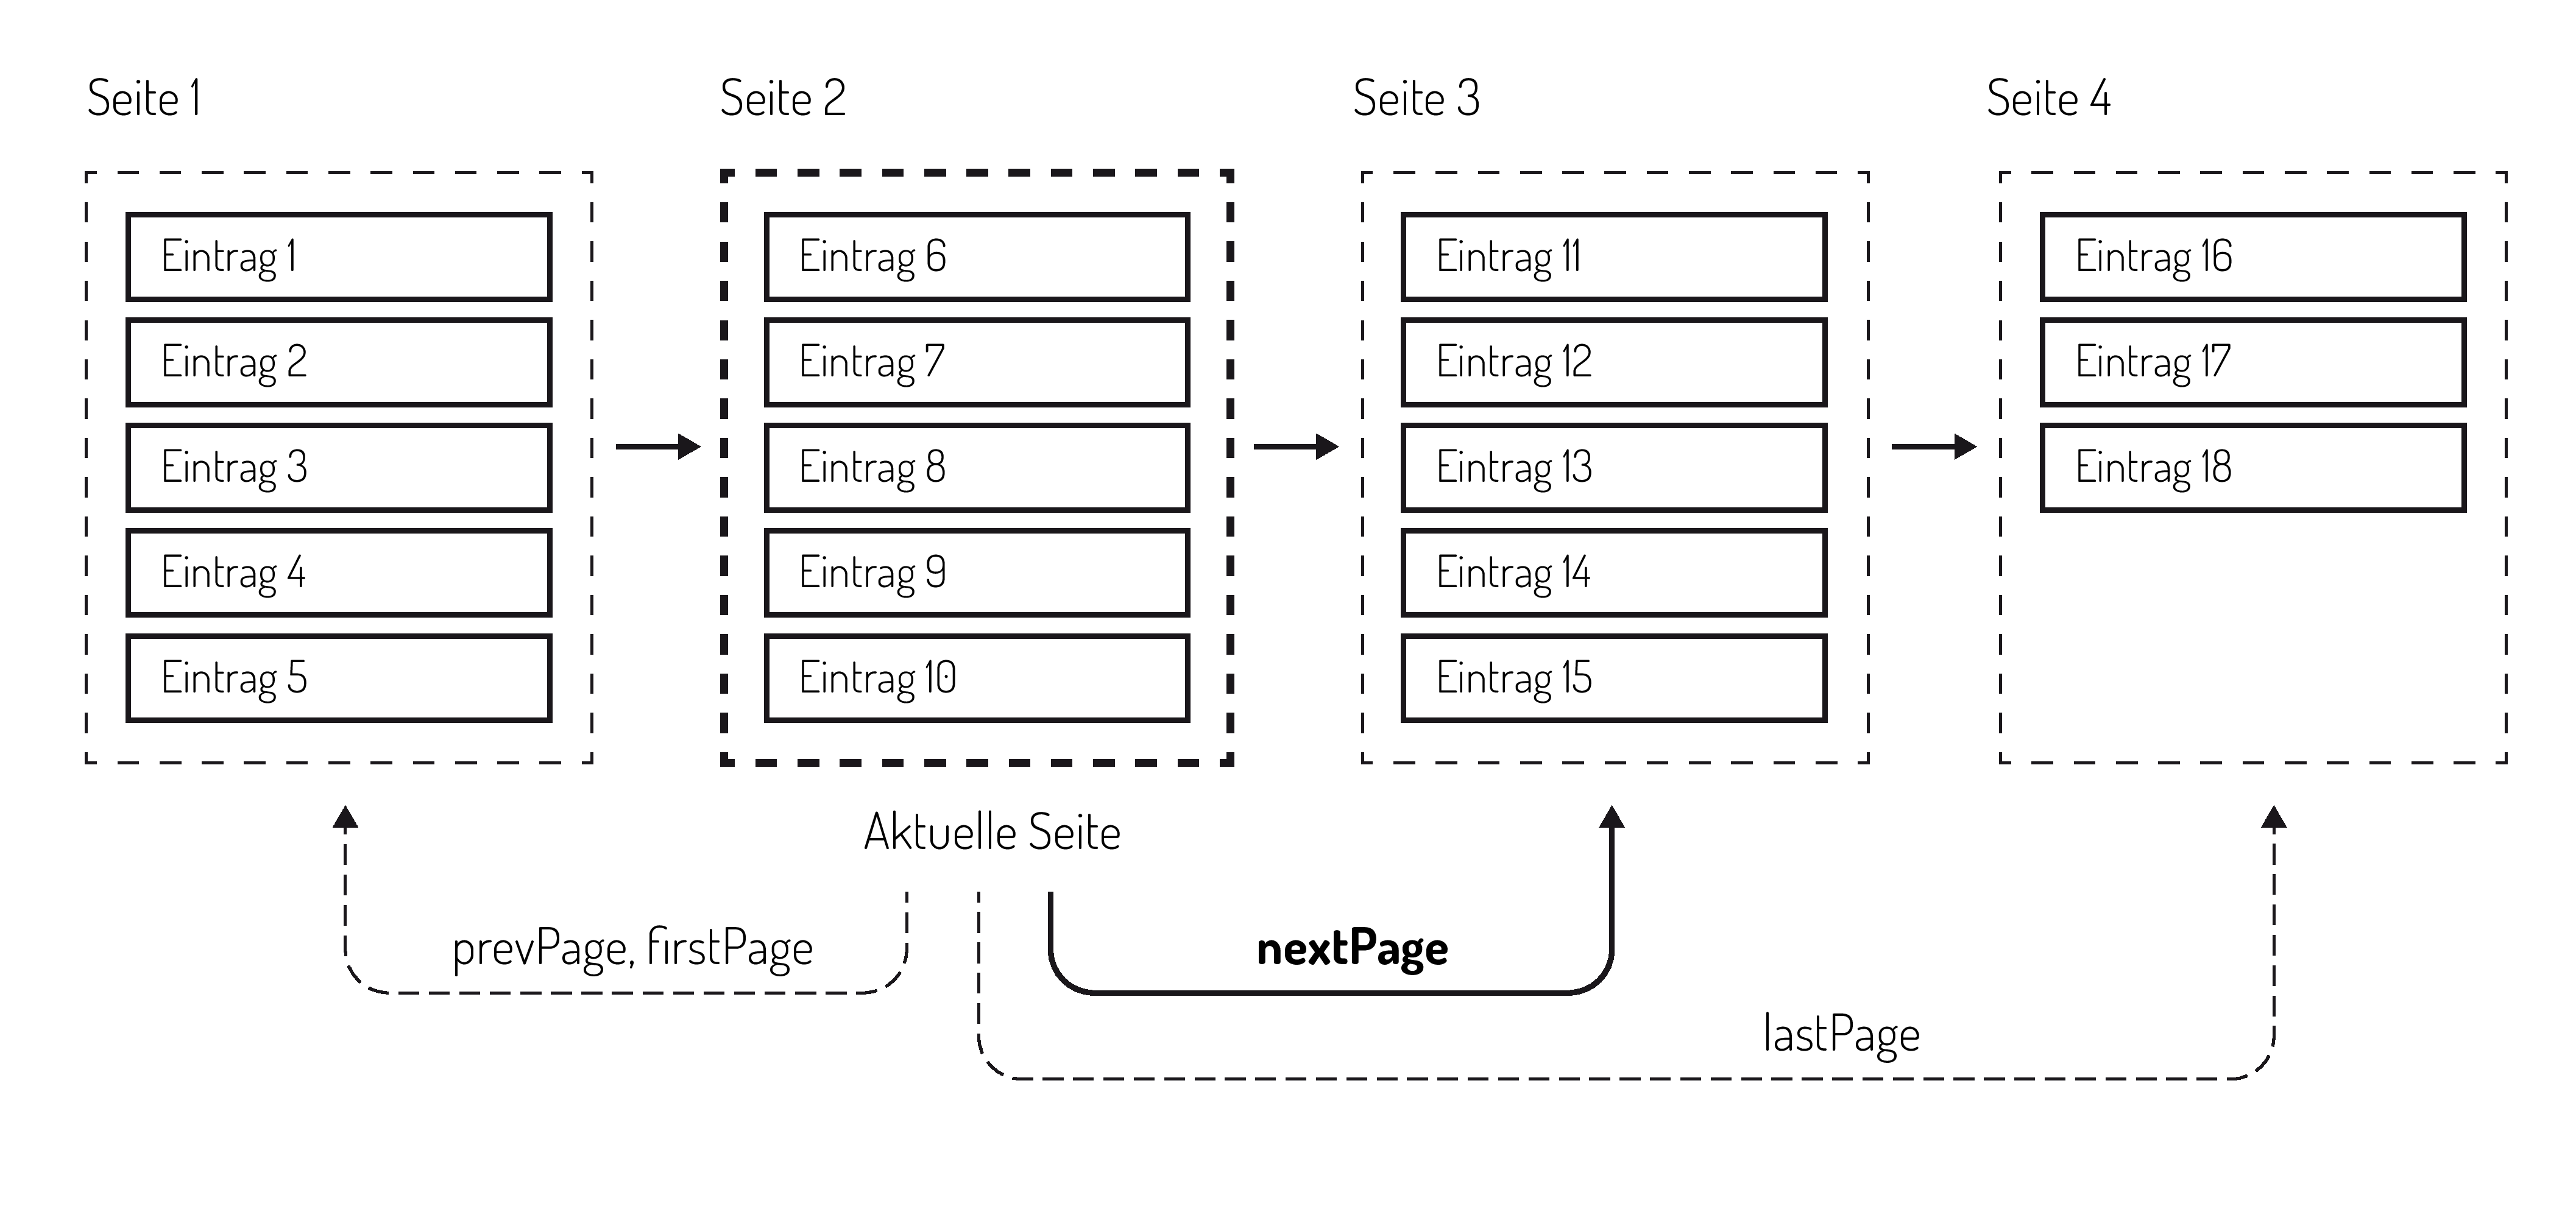
\includegraphics{images/pagination01.png}
\caption{Paginierung: Schematische Darstellung}
\end{figure}

Server-Implementierer entscheiden selbst, wie die URLs zum Abruf
einzelner Listenseiten aufgebaut sind und tragen damit selbst
Verantwortung für die Funktionsweise der Paginierung. Bei der
Entscheidung für eine Form der Implementierung sollten die folgenden
Anforderungen von Clients berücksichtigt werden:

\begin{itemize}
\item
  Es ist davon auszugehen, dass Clients für den gesamten Abruf aller
  Seiten einer Liste längere Zeit benötigen. In der Zwischenzeit kann
  sich der Inhalt der Liste bereits ändern, etwa durch das Hinzukommen
  neuer Einträge. Die Paginierung ist idealerweise so zu implementieren,
  dass sich das Hinzukommen oder Entfernen von Einträgen möglichst nicht
  auf einen Client auswirkt, der aktuell die Liste paginiert, um alle
  Einträge abzurufen. Wir bezeichnen dies als \textbf{stabile
  Paginierung}.
\item
  Eine wesentliche Anforderung an Listen mit Paginierung ist, dass alle
  Einträge der Liste in einer konsistenten Reihenfolge sortiert
  ausgegeben werden MÜSSEN. Das bedeutet, dass die Sortierung beim
  Server im Idealfall anhand einer eindeutigen und unveränderlichen
  Objekteigenschaft vorgenommen wird. Hierfür eignen sich die
  Objekt-URLs, da sie genau diese beiden Anforderungen erfüllen sollten.
\end{itemize}

Über die Sortierung hinaus können bei der Implementierung einer stabilen
Paginierung auf Server-Seite weitere Überlegungen einbezogen werden. Zur
Verdeutlichung soll hier eine ungünstige (unstabile) Form der
Implementierung mit Hilfe einer SQL-Abfrage illustriert werden. Gegeben
sei eine Tabelle \texttt{example}, die einen numerischen Primärschlüssel
\texttt{id} enthält. Nehmen wir an, die erste Seite der Liste wird mit
der Abfrage

\hyperdef{}{objektlistenux5fex3}{\label{objektlistenux5fex3}}
\begin{Shaded}
\begin{Highlighting}[]
\KeywordTok{SELECT} \NormalTok{* }\KeywordTok{FROM} \NormalTok{example }\KeywordTok{ORDER} \KeywordTok{BY} \KeywordTok{id} \KeywordTok{LIMIT} \DecValTok{10} \NormalTok{OFFSET }\DecValTok{0}
\end{Highlighting}
\end{Shaded}

abgerufen und würde 10 Datensätze mit den \texttt{id}s 1 bis 10
zurückliefern. Dann wird die zweite Seite mit der Abfrage

\hyperdef{}{objektlistenux5fex4}{\label{objektlistenux5fex4}}
\begin{Shaded}
\begin{Highlighting}[]
\KeywordTok{SELECT} \NormalTok{* }\KeywordTok{FROM} \NormalTok{example }\KeywordTok{ORDER} \KeywordTok{BY} \KeywordTok{id} \KeywordTok{LIMIT} \DecValTok{10} \NormalTok{OFFSET }\DecValTok{10}
\end{Highlighting}
\end{Shaded}

abgerufen. Sollte nach der ersten, aber vor der zweiten Abfrage
beispielsweise der Datensatz mit der \texttt{id=1} gelöscht worden sein,
liefert die zweite Abfrage Datensätze mit \texttt{id} \textgreater{} 9.
In diesem Fall würde dies nur dazu führen, dass ein Datensatz
(\texttt{id=10}) zweimal ausgegeben wird. Bei ungünstigeren
Konstellationen wäre auch denkbar, dass eine unstabile Paginierung
bewirkt, dass einzelne Datensätze beim Paginieren übergangen werden. Je
nach Bedeutung der fehlenden Datensätze können splche Inkonsistenzen
erhebliche Auswirkungen haben.

Besser wäre es, bei der Paginierung die Eintragsgrenze, bei der eine
Listenseite beginnen soll, explizit zu benennen. Wurden auf der ersten
Listenseite die Datensätze mit den IDs 1 bis 10 ausgegeben, so könnte
der Folgeaufruf, um beim SQL-Beispiel zu bleiben, so aussehen:

\hyperdef{}{objektlistenux5fex5}{\label{objektlistenux5fex5}}
\begin{Shaded}
\begin{Highlighting}[]
\KeywordTok{SELECT} \NormalTok{* }\KeywordTok{FROM} \NormalTok{example }\KeywordTok{WHERE} \KeywordTok{id} \NormalTok{> }\DecValTok{10} \KeywordTok{ORDER} \KeywordTok{BY} \KeywordTok{id} \KeywordTok{LIMIT} \DecValTok{10}
\end{Highlighting}
\end{Shaded}

Die zuvor beschriebenen Anforderungen für die Paginierung von Listen
gelten auch unverändert, wenn der Umfang der Liste durch
Abfrageparameter vom Client eingeschränkt wurde.

\subsubsection{Sortierung}\label{sortierung}

OParl definiert keine Möglichkeit für Clients, auf die Reihenfolge von
Listeneinträgen Einfluss zu nehmen. Von Servern wird die Einhaltung
einiger grundlegender Anforderungen erwartet, die teilweise bereits
erwähnt wurden.

Server SOLLEN generell für eine \textbf{stabile Sortierung} von
Listeneinrägen sorgen. Das heißt, die Sortierung von Einträgen folgt
einem konstanten Prinzip und ändert sich nicht von Abfrage zu Abfrage.
Eine Einfache Möglichkeit, dies Umzusetzen, wäre in vielen Fällen die
Sortierung von Objekten nach ihrer eindeutigen und unveränderlichen ID.

\subsubsection{Filter}\label{filter}

Bei der \emph{externen Listenausgabe} (siehe weiter oben) werden in
Abhängigkeit vom ausgegebenen Objekttyp bestimmte Möglichkeiten geboten,
die Ausgabe von Listen auf eine Teilmenge einzuschränken.

Hierfür sind die URL-Paramter \texttt{startdate} und \texttt{enddate}
vorgesehen. Beide können vom Client unabhängig von einander gesetzt
werden. Sie schränken die Objektmenge anhand auf einen Zeitraum ein, der
entweder einseitig oder beidseitig begrenzt ist. Die Einschränkung
bezieht sich auf ein Bezugsdatum, das vom Objekttyp abhängt.

Der Filter mittels \texttt{startdate} und \texttt{enddate} ist nur auf
Listen mit den folgenden Objekttypen anwendbar:

\begin{itemize}
\itemsep1pt\parskip0pt\parsep0pt
\item
  \texttt{oparl:File}: Bezugsdatum ist hier die Eigenschaft
  \texttt{date} (Erstellungsdatum)
\item
  \texttt{oparl:Meeting}: Bezugsdatum ist hier die Eigenschaft
  \texttt{start} (Startzeitpunkt der Sitzung)
\item
  \texttt{oparl:Paper}: Bezugsdatum ist hier die Eigenschaft
  \texttt{publishedDate} (Veröffentlichungsdatum)
\end{itemize}

Für die genannten Objekttypen MUSS der Server bei externer Litenausgabe
die beschriebenen Filter untertützen.

Die Filter werden vom Client aktiviert, indem der oder die gewünschte(n)
URL-Parameter der vom Server angegebenen URL für die Listenausgabe
hinzugefügt werden. Lautet diese URL für eine Liste von Drucksachen so,

\begin{verbatim}
https://oparl.example.org/papers/
\end{verbatim}

dann kann der Client die folgende URL bilden, um die Ausgabe der Liste
auf Drucksachen einzuschränken, die nach dem 1.1.2014 veröffentlicht
wurden:

\begin{verbatim}
https://oparl.example.org/papers/?startdate=2014-01-01T00%3A00%3A00%2B01%3A00
\end{verbatim}

Der Server interpretiert die Angabe eines \texttt{startdate} so, dass
das Bezugsdatum aller ausgegebenen Objekte gleich oder größer dem im
Parameter angegebenen Datum sein muss. Der Parameter \texttt{enddate}
ist entsprechend so zu interpretieren, dass alle Bezugsdaten der
ausgelieferten Objekte kleiner oder gleich dem angegebenen Wert sein
müssen.

Sind beide Parameter gesetzt, handelt es sich um eine Boolsche
UND-Verknüpfung. Der Server liefert entsprechend nur Objekte aus, deren
Bezugsdatum größer/gleich dem Wert von \texttt{startdate} und
kleiner/gleich dem Wert von \texttt{enddate} ist.

Clients MÜSSEN die Werte von \texttt{startdate} und \texttt{enddate} im
Format xsd:dateTime, also mit Uhrzeit und Zeitzone, angeben (siehe dazu
auch \hyperref[datumux5fzeit]{Datums- und Zeitangaben}) und für eine
entsprechende URL-Kodierung sorgen.

\hyperdef{}{feeds}{\subsection{Feeds}\label{feeds}}

Feeds sind spezielle Arten von \hyperref[objektlisten]{Objektlisten},
für die besondere Anforderungen gelten. Es werden drei verschiedene
Feeds spezifiziert:

\begin{itemize}
\itemsep1pt\parskip0pt\parsep0pt
\item
  Der Feed \emph{Neue Objekte}
\item
  Der Feed \emph{Geänderte Objekte}
\item
  Der Feed \emph{Entfernte Objekte}
\end{itemize}

Der Begriff ``Feed'' ist eine Anlehnung an die weit verbreiteten
RSS-\footnote{RSS 2.0 Specification:
  \url{http://cyber.law.harvard.edu/rss/rss.html}} oder
Atom-Feeds\footnote{Atom ist in RFC4287 spezifiziert:
  \url{http://www.ietf.org/rfc/rfc4287.txt}}, deren Publikationslogik im
Wesentlichen auf der chronologischen Sortierung beruht. Im Unterschied
zu Atom oder RSS ist hier jedoch keine XML-Ausgabe beabsichtigt.

Die Feeds sollen es Clients ermöglichen, schnell und ressourcenschonend
abzufragen, welche Objekte auf dem Server neu hinzugefügt, geändert oder
entfernt wurden. Damit können Clients beispielsweise schnell und einfach
neue Dokumente auffinden und verarbeiten oder entfernte Objekte aus
ihren Caches entfernen und dabei nur ein Mindestmaß an Anfragen
ausführen. Die Feeds unterstützen oder ermöglichen also die
Synchronisation.

Ein OParl-Server SOLL jeden der nachfolgend beschriebenen Feeds
anbieten.

Für alle drei Feeds wird EMPFOHLEN, dass mindestens ein Zeitraum von 365
Tagen abgedeckt wird.

Da Feeds üblicherweise eine große und stetig steigende Anzahl von
Objekten beinhalten können, ist hier die
\hyperref[paginierung]{Paginierung} anzuwenden, wie sie im vorigen
Abschnitt über \hyperref[objektlisten]{Objektlisten} beschrieben wird.

\hyperdef{}{feedux5fneueux5fobjekte}{\subsubsection{Der Feed ``Neue
Objekte''}\label{feedux5fneueux5fobjekte}}

Der Feed für neue Objekte listet die URLs neu hinzugekommener Objekte in
der Reihenfolge des Datums ihrer Erstellung, wobei die jüngsten Objekte
zuerst ausgegeben werden.

Die Definition, was ein ``neues'' Objekt bzw. die ``Erstellung''
bedeutet, kann zwischen Systemen und Objekttypen variieren. So werden
bestimmte Objekte in einigen Systemen zunächst erstellt und erst dann
für die Öffentlichkeit freigegeben. In diesem Fall ist im Sinne dieses
Feeds die Freigabe als Zeitpunkt der Erstellung zu verwenden.

Der Feed SOLL sämtliche Objekttypen umfassen, die in einem System
geführt werden.

Das nachstehende Beispiel zeigt die mögliche Ausgabe des Feeds:

\hyperdef{}{feedux5fex1}{\label{feedux5fex1}}
\begin{Shaded}
\begin{Highlighting}[]
\FunctionTok{\{}
    \DataTypeTok{"items"}\FunctionTok{:} \OtherTok{[}
        \FunctionTok{\{}
            \DataTypeTok{"id"}\FunctionTok{:} \StringTok{"https://oparl.example.org/files/3"}\FunctionTok{,}
            \DataTypeTok{"type"}\FunctionTok{:} \StringTok{"http://oparl.org/schema/1.0/File"}\FunctionTok{,}
            \DataTypeTok{"created"}\FunctionTok{:} \StringTok{"2014-01-07T12:59:01+01:00"}
        \FunctionTok{\}}\OtherTok{,}
        \FunctionTok{\{}
            \DataTypeTok{"id"}\FunctionTok{:} \StringTok{"https://oparl.example.org/papers/21"}\FunctionTok{,}
            \DataTypeTok{"type"}\FunctionTok{:} \StringTok{"http://oparl.org/schema/1.0/Paper"}\FunctionTok{,}
            \DataTypeTok{"created"}\FunctionTok{:} \StringTok{"2014-01-05T18:29:37+01:00"}
        \FunctionTok{\}}\OtherTok{,}
        \FunctionTok{\{}
            \DataTypeTok{"id"}\FunctionTok{:} \StringTok{"https://oparl.example.org/files/5"}\FunctionTok{,}
            \DataTypeTok{"type"}\FunctionTok{:} \StringTok{"http://oparl.org/schema/1.0/File"}\FunctionTok{,}
            \DataTypeTok{"created"}\FunctionTok{:} \StringTok{"2014-01-04T11:26:48+01:00"}
        \FunctionTok{\}}\OtherTok{,}
        \ErrorTok{...}
    \OtherTok{]}\FunctionTok{,}
    \DataTypeTok{"itemsPerPage"}\FunctionTok{:} \ErrorTok{...}\FunctionTok{,}
    \DataTypeTok{"nextPage"}\FunctionTok{:} \ErrorTok{...}
\FunctionTok{\}}
\end{Highlighting}
\end{Shaded}

Die Funktionsweise entspricht grundsätzlich der von gewöhnlichen Listen
mit Paginierung, wie im Kapitel \hyperref[objektlisten]{Objektlisten}
beschrieben.

Davon abweichend gibt der Feed zu jedem neuen Objekt in der Liste unter
\texttt{items} ein JSON-Objekt mit drei Eigenschaften aus:

\begin{itemize}
\itemsep1pt\parskip0pt\parsep0pt
\item
  \texttt{id}: Die URL des neuen Objekts
\item
  \texttt{type}: Die URL des Typs des neuen Objekts
\item
  \texttt{created}: Der Zeitpunkt der Erzeugung des Objekts
\end{itemize}

Der jeweils in der Eigenschaft \texttt{created} ausgegebene Zeitpunkt
SOLL vom Server als Sortierkriterium des Feeds genutzt werden.

\hyperdef{}{feedux5fgeaenderteux5fobjekte}{\subsubsection{Der Feed
``Geänderte Objekte''}\label{feedux5fgeaenderteux5fobjekte}}

Der Feed für geänderte Objekte listet die URLs geänderter Objekte in der
Reihenfolge des Datums ihrer Änderung, wobei das zuletzt geänderte
Objekt zuerst ausgegeben wird.

Die Definition einer ``Änderung'' kann sich zwischen den Objekttypen
unterscheiden. Tendenziell soll die Definition eher weiter ausgelegt
werden, als enger. Als Änderung einer Gruppierung (oparl:Organization)
könnte es beispielsweise verstanden werden, wenn eine neue
Mitgliedschaft zur Organisation hinzukommt. Das Erstellen eines Objekts
(im Sinne des Feeds ``Neue Objekte'') sollte hingegen nicht als Änderung
gewertet werden, um das redundante Erscheinen eines neuen Objekts sowohl
im Feed ``Neue Objekte'' als auch im Feed ``Geänderte Objekte'' zu
vermeiden.

Auch hier SOLL der Feed sämtliche Objekttypen umfassen, die in einem
System geführt werden.

\hyperdef{}{feedux5fex2}{\label{feedux5fex2}}
\begin{Shaded}
\begin{Highlighting}[]
\FunctionTok{\{}
    \DataTypeTok{"items"}\FunctionTok{:} \OtherTok{[}
        \FunctionTok{\{}
            \DataTypeTok{"id"}\FunctionTok{:} \StringTok{"https://oparl.example.org/files/2"}\FunctionTok{,}
            \DataTypeTok{"type"}\FunctionTok{:} \StringTok{"http://oparl.org/schema/1.0/File"}\FunctionTok{,}
            \DataTypeTok{"modified"}\FunctionTok{:} \StringTok{"2014-01-08T14:28:31+01:00"}
        \FunctionTok{\}}\OtherTok{,}
        \FunctionTok{\{}
            \DataTypeTok{"id"}\FunctionTok{:} \StringTok{"https://oparl.example.org/papers/0"}\FunctionTok{,}
            \DataTypeTok{"type"}\FunctionTok{:} \StringTok{"http://oparl.org/schema/1.0/Paper"}\FunctionTok{,}
            \DataTypeTok{"modified"}\FunctionTok{:} \StringTok{"2014-01-08T12:14:27+01:00"}
        \FunctionTok{\}}\OtherTok{,}
        \FunctionTok{\{}
            \DataTypeTok{"id"}\FunctionTok{:} \StringTok{"https://oparl.example.org/files/1"}\FunctionTok{,}
            \DataTypeTok{"type"}\FunctionTok{:} \StringTok{"http://oparl.org/schema/1.0/File"}\FunctionTok{,}
            \DataTypeTok{"modified"}\FunctionTok{:} \StringTok{"2014-01-06T17:01:00+01:00"}
        \FunctionTok{\}}\OtherTok{,}
    \OtherTok{]}\FunctionTok{,}
    \DataTypeTok{"itemsPerPage"}\FunctionTok{:} \ErrorTok{...}\FunctionTok{,}
    \DataTypeTok{"nextPage"}\FunctionTok{:} \ErrorTok{...}
\FunctionTok{\}}
\end{Highlighting}
\end{Shaded}

Das Ausgabeformat entspricht weitgehend dem des Feeds ``Neue Objekte'',
jedoch heißt hier die Eigenschaft für den Zeitpunkt der letzten Änderung
\texttt{modified}. Entsprechend gilt, dass der als \texttt{modified}
ausgegebene Zeitpunkt als Sortierkriterium der Liste gelten SOLL.

\hyperdef{}{feedux5fentfernteux5fobjekte}{\subsubsection{Der Feed
``Entfernte Objekte''}\label{feedux5fentfernteux5fobjekte}}

Der Feed für entferne Objekte listet die URLs entfernter Objekte in der
Reihenfolge des Datums ihrer Entfernung auf, wobei die zuletzt
entfernten Objekte zuerst ausgegeben werden.

Mit ``Entfernung'' ist im Sinne dieses Feeds die Löschung eines Objekts,
aber auch die Depublikation oder das Beenden der öffentlichen
Verfügbarkeit gemeint.

Client-Implementierer sind angehalten, diesen Feed zu nutzen, um
beispielsweise depublizierte Dokumente aus ihren lokalen Caches zu
entfernen.

\hyperdef{}{feedux5fex3}{\label{feedux5fex3}}
\begin{Shaded}
\begin{Highlighting}[]
\FunctionTok{\{}
    \DataTypeTok{"items"}\FunctionTok{:} \OtherTok{[}
        \FunctionTok{\{}
            \DataTypeTok{"id"}\FunctionTok{:} \StringTok{"https://oparl.example.org/people/22"}\FunctionTok{,}
            \DataTypeTok{"removed"}\FunctionTok{:} \StringTok{"2013-11-11T11:11:00+01:00"}
        \FunctionTok{\}}\OtherTok{,}
        \ErrorTok{...}
    \OtherTok{]}\FunctionTok{,}
    \DataTypeTok{"itemsPerPage"}\FunctionTok{:} \ErrorTok{...}\FunctionTok{,}
    \DataTypeTok{"nextPage"}\FunctionTok{:} \ErrorTok{...}
\ErrorTok{]}
\end{Highlighting}
\end{Shaded}

Die Eigenschaft zur Angabe des Entfernungszeitpunkts heißt hier
\texttt{removed} und SOLL, analog zu den beiden anderen Feeds, als
Sortierkriterium der Liste verwendet werden.

Im Unterschied zu den beiden zuvor beschriebenen Feeds wird im Feed
``Gelöschte Objekte'' keine Eigenschaft \texttt{type} am jeweiligen
Objekt ausgegeben.

Clients SOLLEN vermeiden, die URLs der jeweiligen Einträge erneut
aufzurufen.

\subsection{Daten Dump / bulk download}\label{daten-dump-bulk-download}

Als Alternative zu dem eher fein-granularen Zugriff auf einzelne
OParl-Objekte kann es sinnvoll sein, wenn alle Objekte in einem Vorgang
abgerufen werden können. Gründe dafür können sein:

\begin{itemize}
\item
  \begin{enumerate}
  \def\labelenumi{\alph{enumi}.}
  \setcounter{enumi}{25}
  \itemsep1pt\parskip0pt\parsep0pt
  \item
    B. für Auswertungen wird ein großer Teil aller Objekte benötigt
  \end{enumerate}
\item
  Anzahl erforderlicher http-Zugriffe sinkt drastisch
\item
  die Last auf dem Server (z. B. für Datenbank) kann reduziert werden
\end{itemize}

Für die Implementierung gibt es mehrere Anforderungen: * weitgehende
Nutzung ohnehin bereits in OParl genutzter Techniken * Verwendung
etablierter Vokabulare

Bei Betrachtung der OParl-Daten als Tripel geht es hier um eine Abfrage
nach allen Objekten, deren Subjekt, Prädikat und Objekt nicht
eingeschränkt ist.
\textsubscript{\textsubscript{\textsubscript{\textsubscript{\textsubscript{
https://oparl.example.org/ldf?subject=\&predicate=\&object= }}}}}

Zum Vergleich: Bei einer Abfrage von
\hyperref[objektlisten]{Objektlisten} sind Subjekt und Prädikat durch
die Abfrage festgelegt, nur das Objekt ist variabel.

Für die Spezifikation des Formats der downloadbaren Dateien wird also
auf das Objektlisten-Format zurückgegriffen.

Wenn das Ergebnis dieser Abfrage in eine Datei geschrieben und als
solche zum Download angeboten wird, dann kann und soll auf
\hyperref[paginierung]{Paginierung} in dieser Datei jedoch verzichtet
werden, da diesei Daten nur stören würden.

TODO: Beispiel und Besonderheiten TODO: SOLL-Anforderung

In dieser Version von OParl werden keine Festlegungen getroffen, wie ein
Client über die URLs der downloadbaren Dateien informiert wird. In Frage
kommen aber z. B. Links, die auf HTML-Seiten plaziert werden.

\hyperdef{}{dateizugriff}{\subsection{Dateizugriff}\label{dateizugriff}}

Mit dem Begriff ``Datei'' sind im Sinne dieser Spezifikation alle
Ressourcen gemeint, die von einem OParl-Server zur Verfügung gestellt
werden und deren Metadaten über die JSON-API als
\hyperref[oparlux5fdocument]{\texttt{oparl:File}} abgerufen werden
können. Es handelt sich dabei beispielsweise um Textdokumente im
PDF-Format, Abbildungen im JPEG- oder PNG-Format etc., die wesentliche
Inhalte der parlamentarischen Informationen im OParl-System ausmachen.

In Bezug auf die Datenvolumen, die der Verkehr zwischen OParl-Servern
und -Clients ausmacht, kommt dem Dateizugriff eine besondere Bedeutung
zu. Daher formuliert OParl diesbezüglich einige Anforderungen, die
helfen sollen, unnötigen Datentransfer zu vermeiden.

Detail zu sämtlichen angesprochenen Mechanismen sind in den
verschiedenen Teilen der HTTP-1.1-Spezifikation\footnote{vgl.
  \url{http://tools.ietf.org/html/rfc7230},
  \url{http://tools.ietf.org/html/rfc7231},
  \url{http://tools.ietf.org/html/rfc7232}} zu finden.

\subsubsection{GET und HEAD Anfragen}\label{get-und-head-anfragen}

Grundsätzlich gilt, dass jede Datei mittels HTTP-Anfrage unter
Verwendung der HTTP-Methode \texttt{GET} abrufbar sein MUSS. Um Clients
zusätzlich die Überprüfung einer Datei zu ermöglichen, MUSS vom Server
außerdem die HTTP-Methode \texttt{HEAD} unterstützt werden. Gemäß
HTTP-Spezifikation gibt der Server in diesem Fall nur die
Antwort-Header, nicht aber den eigentlichen Inhalt der angefragten
Ressource, aus.

Die URLs zum Abruf der einzelnen Datei (wahlweise mittels GET oder HEAD)
stellt der Server dem Client in den Daten des Metadaten-Objekts zur
Verfügung. Details finden sich in der Schema-Beschreibung zu
\hyperref[oparlux5fdocument]{\texttt{oparl:File}}.

\subsubsection{Allgemeiner Zugriff und expliziter
Download}\label{allgemeiner-zugriff-und-expliziter-download}

Mit der im \texttt{oparl:File} ZWINGEND anzugebenden Eigenschaft
\texttt{accessUrl} liefert der Server dem Client eine URL, die wir hier
nachfolgend als \emph{Zugriffs-URL} bezeichnen. Diese URL dient dem
allgemeinen Zugriff auf die Datei. Wie der Client dem Endnutzer diesen
Zugriff genau ermöglicht, ist nicht Sache der OParl-Spezifikation.

Im Unterschied dazu KANN der Server dem Client in der Eigenschaft
\texttt{downloadUrl} eine weitere URL anbieten, hier \emph{Download-URL}
genannt. Diese dient im Gegensatz zur Zugriffs-URL speziell zum
Herunterladen und Speichern der Datei in einem Dateisystem des
Endnutzers. Bei Zugriff auf die Download-URL MUSS der Server in der
HTTP-Antwort einen \texttt{Content-Disposition} Header senden.\footnote{vgl.
  RFC2138 \url{http://www.ietf.org/rfc/rfc2183}} Dieser Header MUSS als
ersten Parameter den Typ \texttt{attachment} sowie den
\texttt{filename}-Parameter mit dem Namen der Datei enthalten.

Beispiel:

\begin{verbatim}
Content-Disposition: attachment; filename="2014-08-22 Rat Wortprotokoll.pdf"
\end{verbatim}

FRAGE: Sind in Dateinamen sinnvoll?

Der in diesem Header kommunizierte Dateiname ist als Vorschlag an die
Nutzerin zu verstehen, die Datei unter diesem Namen zu speichern.
Entsprechend sind Abwägungen bezüglich der Verständlichkeit,
Leserlichkeit und Einzigartigkeit des Dateinamens, aber auch in Hinblick
auf den verwendeten Zeichenumfang zu berücksichtigen. Es wird EMPFOHLEN,
den Dateinamen ausschließlich aus dem ASCII-Zeichenvorrat zu bilden.
FRAGE: Ist die Beschränkung auf ASCII und damit der Verzicht z.B. auf
Umlaute erforderlich?

Im Unterschied zum Zugriff auf die Download-URL DARF der Server beim
Zugriff auf die Zugriffs-URL KEINEN \texttt{Content-Disposition} Header
mit Parameter \texttt{attachment} senden.

\subsubsection{Obligatorische und empfohlene
Header}\label{obligatorische-und-empfohlene-header}

Ziel ist, dem Client möglichst flexible Möglichkeiten zu geben, einen
Cache zu überprüfen bzw. zu aktualisieren und vermeidbare Anfragen einer
Ressource zu vermeiden. Um dies zu unterstützen, können laut
HTTP-Spezifikationen unterschiedliche Header zum Einsatz kommen.

Die Auslieferung eines \texttt{Last-Modified}-Headers gilt für alle
OParl-Server beim Zugriff auf eine Datei-URL, sei es Download- oder
Zugriffs-URL, als ZWINGEND.

Darüber hinaus EMPFEHLEN wir, bei Anfrage einer Datei die folgenden
Header auszuliefern:

\begin{itemize}
\itemsep1pt\parskip0pt\parsep0pt
\item
  \texttt{Content-Length}: Die Größe des Dateiinhalts
\item
  \texttt{ETag}: Entity Tag
\end{itemize}

\subsubsection{Conditional GET}\label{conditional-get}

Unter einem ``Conditional GET'' versteht man im HTTP-Kontext die
Möglichkeit des Clients, die Anfrage einer Ressource mit einer Bedingung
zu verknüpfen. Der Server beantwortet die Anfrage nur dann mit einer
vollständigen HTTP-Antwort, wenn die Bedingung erfüllt ist. Andernfalls
enthält die Anfrage lediglich den Header; der HTTP Status-Code SOLL in
diesem Fall ``304'' lauten (für ``nicht geändert''). Dies dient der
Schonung von Ressourcen.

Für einen OParl-Server wird EMPFOHLEN, die nachstehenden Varianten des
Conditional GET zu unterstützen:

\begin{itemize}
\item
  \texttt{If-Modified-Since}: Der Client sendet mit der Anfrage als
  Bedingung ein Datum. Nur wenn die angefragte Datei zuletzt \emph{nach}
  diesem Datum geändert wurde, wird der Dateiinhalt mit der Antwort
  ausgeliefert.
\item
  \texttt{If-None-Match}: Erlaubt die Formulierung der Bedingung anhand
  eines Entity-Tags.
\end{itemize}

\subsubsection{Zustandsloser
Dateizugriff}\label{zustandsloser-dateizugriff}

Die Anforderung, dass die OParl-API zustandslos arbeitet (vgl.
\hyperref[restful]{RESTful}\{\#restful\}), hat ZWINGEND auch für den
Abruf von Dateien zu gelten. Es DÜRFEN daher keine Session-spezifischen
URLs oder Ähnliches für den Dateizugriff gebildet werden.

Damit wird erreicht, dass Clients die Zugriffs-URLs aus dem
\texttt{oparl:File} für längere Zeit speichern bzw. cachen können.

\subsubsection{Weiterleitungen}\label{weiterleitungen}

Es ist im Rahmen dieser Spezifikation problemlos möglich, die Anfrage an
eine Datei-URL mit einer HTTP-Weiterleitung zu beantworten, um dem
Client eine andere URL zum Zugriff mitzuteilen.

In diesem Fall wird dringend EMPFOHLEN, die Unterscheidung der Bedeutung
der HTTP-Status-Codes \texttt{301} und \texttt{307} zu beachten.

\begin{itemize}
\item
  \texttt{301} SOLL verwendet werden, wenn die vom Client angefragte URL
  auch zukünftig nicht mehr gültig sein wird. Clients erhalten damit das
  Signal, die bisherige URL zu verwerfen und zukünftig die neue, vom
  Server in der Antwort mitgeteilte zu verwenden.
\item
  \texttt{307} SOLL verwendet werden, wenn die vom Client genutzte URL
  nur temporär auf eine bestimmte andere URL weiter leitet. Clients
  werden so aufgefordert, die vorhandene URL auch bei zukünftigen
  Anfragen zu nutzen.
\end{itemize}

\subsubsection{Entfernte Dateien}\label{entfernte-dateien}

Beim Zugriff auf eine Datei, die zuvor einmal abrufbar war, es
inzwischen jedoch nicht mehr ist, SOLL die HTTP-Antwort des Servers den
spezifischen Status-Code \texttt{410} tragen.

\hyperdef{}{contentux5fnegotiation}{\subsection{Content
Negotiation}\label{contentux5fnegotiation}}

Das Prinzip \emph{Content Negotiation} wurde bereits in
RFC2295\footnote{RFC2295: \url{http://tools.ietf.org/html/rfc2295}}
beschrieben und bedeutet, dass WWW-Server eine Ressource in
verschiedenen Formaten bereithalten können und Clients die Möglichkeit
haben, eine Vorliebe für ein bestimmtes Format zu übermitteln. Auch die
HTTP-1.1-Spezifikation\footnote{RFC7231:
  \url{http://tools.ietf.org/html/rfc7231\#section-3.4}} schließt
Content Negotiation ein.

Die Idee hinter Content Negotiation ist, dass ein Client die von ihm
akzeptierten Repräsentationen im \texttt{Accept}-Header der HTTP-Anfrage
mitsendet, damit der Server gemäß Spezifikation die am besten passende
und von ihm unterstützte Repräsentation an den Client ausliefert.

Grundanforderung der vorliegenden Spezifikation an OParl-Clients ist,
dass sie bei jeder Anfrage an einen OParl-Server einen Accept-Header mit
dem Mime-Type \texttt{application/ld+json} senden MÜSSEN, es sei denn,
es handelt sich um einen \hyperref[dateizugriff]{Dateizugriff}.

Im Kontext von OParl soll durch Unterstützung von Content Negotiation
ermöglicht werden, dass die URLs von OParl-Objekten auch von WWW-Clients
aufgerufen werden können, die nicht unmittelbar in Kenntnis der
OParl-Spezifikation entwickelt wurden.

Ein Beispiel für einen solchen Client wäre ein üblicher Browser. Ruft
dieser die URL einer Drucksache (OParl-Objekttyp \texttt{oparl:Paper})
auf, sendet er entweder keinen \texttt{Accept}-Header oder aber einen
solchen, der eine Bevorzugung von Inhaltstypen wie HTML angibt.

Der Server DARF nun, da kein Accept-Header mit dem Typ
\texttt{application/ld+json} gesendet wurde, dem Client eine alternative
Version der Information über die Drucksache ausliefern, beispielsweise
eine HTML-Ansicht.

Ein Server DARF eine alternative Inhaltsform auch in Form einer
HTTP-Weiterleitung anbieten.

\subsection{HTTP-Kompression}\label{http-kompression}

Die zwischen Servern und Clients übertragenen Datenvolumen SOLLEN mit
Hilfe von Kompressionsverfahren reduziert werden, wenn sowohl der Client
als auch der Server dies unterstützen. Dabei kommt das in HTTP
1.1\footnote{RFC7231 Section 5.3.4:
  \url{http://tools.ietf.org/html/rfc7231\#section-5.3.4}} beschriebene
Verfahren zum Einsatz.

HTTP 1.1 stellt drei komprimierte Kodierungen vor, wobei die Liste durch
Registrierung neuer Verfahren bei der IANA erweitert werden kann. Diese
sind:

\begin{itemize}
\itemsep1pt\parskip0pt\parsep0pt
\item
  gzip
\item
  compress
\item
  deflate
\end{itemize}

Server-Implementierer SOLLEN mindestens eines dieser drei Verfahren
unterstützen, wenn Clients dies mittels Accept-Encoding-Header anfragen.

Die Verwendung von HTTP-Kompression ist grundsätzlich sowohl bei
JSON-Daten als auch bei Dateizugriffen möglich. Bei Dateizugriffen sind
die zu erwartenden Einsparungen beim Datenvolumen stark abhängig vom
jeweiligen Dateifomat. Bei bereits komprimierten Dateien wie
beispielsweise OpenOffice oder PDF lassen sich oft nur geringe oder gar
keine weiteren Ersparnisse erzielen. Daher DARF grundsätzlich der Server
in solchen Fällen eine unkomprimierte HTTP-Antwort senden, auch wenn der
Client ein unterstütztes Kompressionsverfahren angefragt hat.

\subsection{Ausnahmebehandlung}\label{ausnahmebehandlung}

Nicht immer kann ein Server die Anfrage eines Clients erfolgreich, also
im Sinne der Anfrage, behandeln und eine entsprechende Antwort liefern.
Beispiele für solche Ausnahmefälle könnten sein (ohne Anspruch auf
Vollständigkeit):

\begin{itemize}
\item
  Eine angefragte Ressource existiert nicht
\item
  Eine angefragte Ressource existiert nicht mehr
\item
  Der Client nutzt eine nicht unterstützte HTTP-Methode, z. B.
  \texttt{POST}
\item
  Der Client nutzt einen nicht interpretierbaren URL-Parameter
\end{itemize}

Die HTTP-1.1-Spezifikation sieht für derartige und weitere Ausnahmefälle
zahlreiche spezifische Status-Codes vor, die hier nicht wiederholt
werden sollen. Verallgemeinernd lautet die Anforderung an jeden
OParl-Server, dass diese Ausnahmen mit den entsprechenden
HTTP-Status-Codes beantworten SOLLEN. Damit wird Client-Entwicklern die
Möglichkeit gegeben, diese Fälle entsprechend zu behandeln.

Clients DÜRFEN darüber hinaus nicht davon ausgehen, dass mit der
HTTP-Antwort im Fall einer Ausnahme noch weitere verwertbare
Informationen wie z. B. eine Fehlermeldung gesendet werden.

\subsection{Liste reservierter
URL-Parameter}\label{liste-reservierter-url-parameter}

Die in dieser Liste enthaltenen Zeichenketten haben eine reservierte
Bedeutung und stehen bei Implementierungen eines OParl-Servers nicht
mehr für die freie Verwendung in URLs zur Verfügung.

\begin{description}
\itemsep1pt\parskip0pt\parsep0pt
\item[\texttt{callback}:]
Mit diesem Parameter wird die JSONP-Ausgabe aktiviert. Mehr dazu im
Abschnitt \hyperref[jsonp]{JSONP}.
\item[\texttt{startdate}:]
Parameter für die Einschränkung einer Abfrage anhand eines Datums bzw.
einer Zeitangabe.
\item[\texttt{enddate}:]
Parameter für die Einschränkung einer Abfrage anhand eines Datums bzw.
einer Zeitangabe.
\item[\texttt{listformat}:]
Parameter zur Steuerung der Listenausgabe. Siehe dazu:
\hyperref[objektlistenux5flistformat]{Objektlisten: Kompakte und
vollständige Form}
\item[\texttt{subject}:]
Eventuelle Verwendung für Linked Data Fragments
\item[\texttt{predicate}:]
Eventuelle Verwendung für Linked Data Fragments
\item[\texttt{object}:]
Eventuelle Verwendung für Linked Data Fragments
\end{description}

\section{Schema}\label{schema}

Dieses Kapitel beschreibt das Schema von OParl. Das Schema bildet das
Datenmodell der OParl-Architektur ab. Es definiert, welche Objekttypen
über eine OParl-API abgerufen werden können und welche Eigenschaften
diese Objekttypen haben dürfen und müssen. Darüber hinaus ist im Schema
auch festgelegt, in welcher Beziehung verschiedene Objekttypen zu
einander stehen.

\begin{figure}[htbp]
\centering
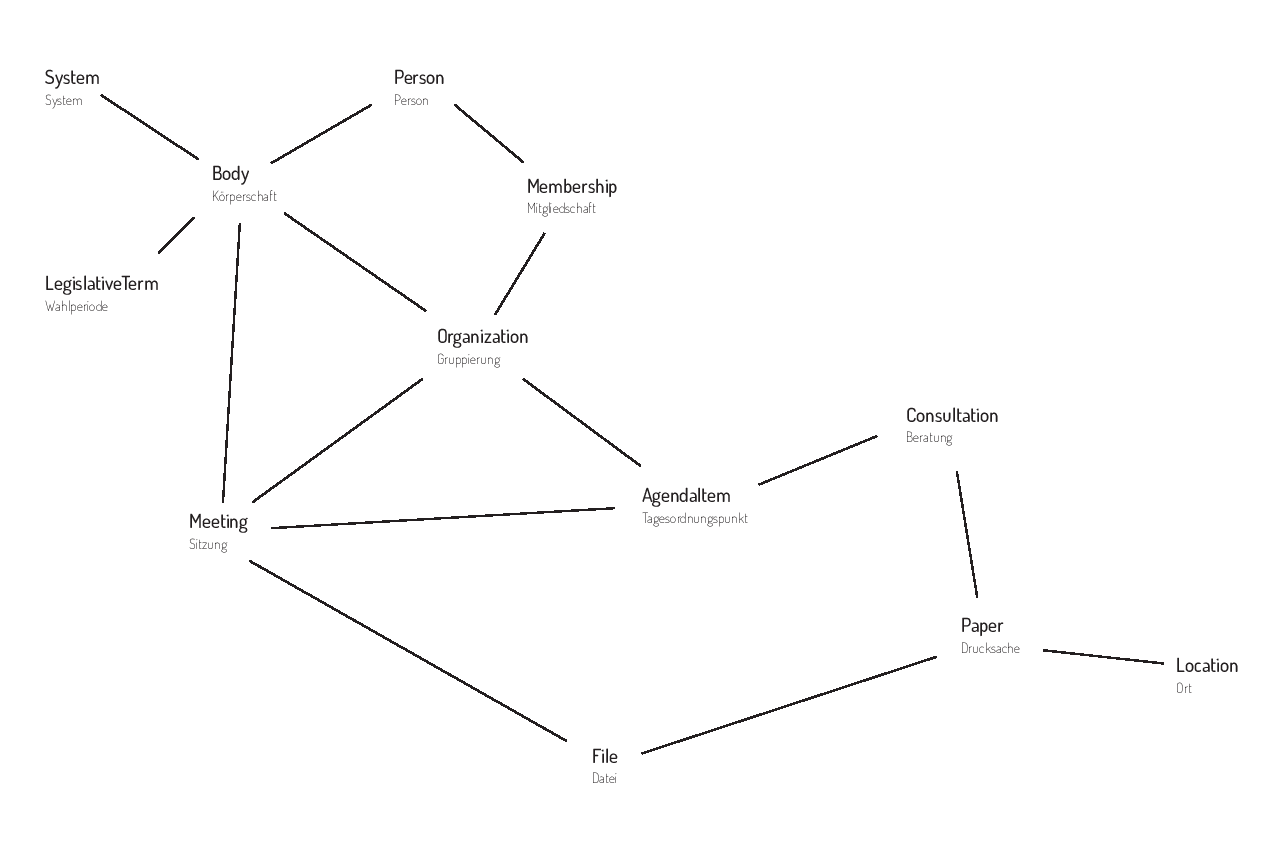
\includegraphics{images/objekttypen_graph.png}
\caption{OParl Objekttypen: Ein Überblick}
\end{figure}

\subsection{Übergreifende Aspekte}\label{uxfcbergreifende-aspekte}

\subsubsection{Unicode-Zeichenketten als
Standard}\label{unicodeux5fzeichenketten}

Die Schema-Beschreibung gibt zu jeder Eigenschaft eines Objekttypen an,
welchen Typ der Wert dieser Eigenschaft haben muss.

Sofern keine Typ-Angabe zu einer Eigenschaft vorhanden ist, oder die
Typ-Angabe \texttt{String} oder \texttt{xsd:string} lautet, werden
Unicode-Zeichenketten als Datentyp erwartet.

\subsubsection{\texttt{null}-Werte und ``leere''
Werte}\label{null-werte-und-leere-werte}

JSON erlaubt es grundsätzlich, Eigenschaften mit dem Wert \texttt{null}
zu versehen. Ein \emph{Client} MUSS \texttt{null}-Werte tolerieren und
SOLL diese Eigenschaften nicht anders anzeigen, als nicht vorhandene
Eigenschaften.

Entsprechendes gilt für leere Wertemengen oder -listen, also
\texttt{{[}{]}}, und leere Objekte, also \texttt{\{\}}.

Dafür gibt es zwei Gründe. Einerseits wird dadurch die Umgehung des
Zwangs zur Angabe von Werten bei ZWINGENDEN Eigenschaften
ausgeschlossen. Andererseits enthalten solche Leerkonstruktionen keine
verwendbare Information.

\subsubsection{URLs der Eigenschaften}\label{urls-der-eigenschaften}

Jede Eigenschaft ist unter einer URL identifizierbar.

\subsubsection{Verwendung externer Eigenschaften / abgeleitete
Eigenschaften}\label{verwendung-externer-eigenschaften-abgeleitete-eigenschaften}

Verschiedene Eigenschaften sind nicht in OParl selbst definiert, sondern
in anderen externen Vokabularen. Dabei legt die Oparl-Spezifikation
jeweils fest, ob die Original-Eigenschaft verwendet wird oder ob für
OParl eine abgeleitete Eigenschaft verwendet wird.

So ist für eine Eigenschaft
\texttt{classification" von Gruppierungen eine Verwendung von}org:classification\texttt{ebenso denkbar wir die Verwendung von}oparl:classification`.
Im zweiten Fall wird die Eigenschaft als Untereigenschaft der
Ausgangseigenschaft definiert. Die Ausgangseigenschaft wird dann jeweils
hinter ``Abgeleitet von:'' angeben.

Auf die Bedeutung dieses Unterschiedes und der
Untereigenschafts-Beziehung wird an dieser Stelle nicht weiter
eingegangen Stichwort: \texttt{owl:subPropertyOf}). Unterschiede kann es
z.B. bei den Wertebereichen geben.

Der Name der Ausdgangseigenschaft muss nicht übernommen werden. In OParl
wird aber in der Regel der jeweilige Ausgangsname verwendet.

\subsubsection{Kardinalität}\label{kardinalituxe4t}

Viele Eigenschaften erlauben es, entweder einen einzelnen Wert (z. B.
eine Zeichenkette, eine URL, eine Zahl) oder alternativ eine Liste mit
mehreren Elementen des jeweils erlaubten Typs auszugeben. Die
entsprechende Regel ist in der Schema-Beschreibung unter dem Stichwort
\emph{Kardinalität} angegeben. Dabei sind verschiedene Angaben zur
Eigenschaft möglich:

\begin{itemize}
\item
  0 bis 1: OPTIONAL und MUSS NICHT gesetzt sein. Wenn sie gesetzt ist,
  DARF sie genau einen Wert haben.
\item
  1: MUSS gesetzt sein und genau einen Wert haben.
\item
  0 bis *: OPTIONAL und MUSS NICHT gesetzt sein. Wenn sie gesetzt ist,
  DARF sie beliebig viele Werte haben.
\item
  1 bis *: MUSS vorhanden sein, es MUSS mindestens ein Wert gesetzt
  sein. Es DÜRFEN auch mehrere Werte vorhanden sein.
\end{itemize}

Zur Ausgabe von Listen innerhalb eines Objekts sowie über eigene URLs
finden sich ausführlichere Erläuterungen im Abschnitt
\hyperref[objektlisten]{Objektlisten}.

\hyperdef{}{datumux5fzeit}{\subsubsection{Datums- und
Zeitangaben}\label{datumux5fzeit}}

Für Datum und Zeit werden die in XML-Schema festgelegten Typen verwendet
(was nicht bedeutet, dass in OParl XML verwendet wird).

Für ein Datum wird http://www.w3.org/TR/xmlschema-2/\#date verwendet und
für eine Zeit http://www.w3.org/TR/xmlschema-2/\#dateTime. Dabei wird
ein Datum (ein Tag ohne Uhrzeit) ohne Zeitzone und ein Datum mit Zeit
mit Zeitzone angegeben, denn nur damit ist die Uhrzeit weltweit
eindeutig ohne zusätzlich auf den Ort einer Sitzung o. ä. Bezug nehmen
zu müssen.

Diese Spezifikationen stützen sich auf RFC 3339\footnote{RFC3339:
  \url{http://www.ietf.org/rfc/rfc3339.txt}}) und RFC 3339 wiederum auf
ISO 8601.

In der vorliegenden Spezifikation verwenden wir den Präfix \texttt{xsd},
um Eigenschaften aus der XMLSchema-Spezifikation zu
referenzieren.\footnote{Der Präfix ``xsd'' steht somit für die URL
  \url{http://www.w3.org/2001/XMLSchema\#}}. Datums- und Zeittyp werden
entsprechend in diesem Dokument als \texttt{xsd:date} bzw.
\texttt{xsd:dateTime} bezeichnet.

\hyperdef{}{vokabulareux5fklassifizierung}{\subsubsection{Vokabulare zur
Klassifizierung}\label{vokabulareux5fklassifizierung}}

Einige Objekttypen besitzen Eigenschaften zum Zweck der Klassifizierung
von Objekten. Im Einzelnen sind dies:

\begin{itemize}
\itemsep1pt\parskip0pt\parsep0pt
\item
  \texttt{classification} des Objekttyps
  \hyperref[oparlux5forganization]{\texttt{oparl:Organization}}
\item
  \texttt{documentRole} des Objekttyps
  \hyperref[oparlux5fdocument]{\texttt{oparl:File}}
\item
  \texttt{formOfAddress} des Objekttyps
  \hyperref[oparlux5fperson]{\texttt{oparl:Person}}
\item
  \texttt{keyword} in mehreren Objekttypen
\item
  \texttt{paperType} des Objekttyps
  \hyperref[oparlux5fpaper]{\texttt{oparl:Paper}}
\item
  \texttt{post} des Objekttyps
  \hyperref[oparlux5forganization]{\texttt{oparl:Organization}}
\item
  \texttt{result} des Objekttyps
  \hyperref[oparlux5fagendaitem]{\texttt{oparl:AgendaItem}}
\item
  \texttt{role} des Objekttyps
  \hyperref[oparlux5fconsultation]{\texttt{oparl:Consultation}}
\item
  \texttt{role} des Objekttyps
  \hyperref[oparlux5fmembership]{\texttt{oparl:Membership}}
\item
  \texttt{role} des Objekttyps
  \hyperref[oparlux5fperson]{\texttt{oparl:Person}}
\item
  \texttt{status} des Objekttyps
  \hyperref[oparlux5fperson]{\texttt{oparl:Person}}
\item
  \texttt{title} des Objekttyps
  \hyperref[oparlux5fperson]{\texttt{oparl:Person}}
\end{itemize}

Diese Eigenschaften können als Wert wahlweise einfache Zeichenketten
(Strings) haben, z. B. \texttt{"Beantwortung einer Anfrage"} oder aber
URLs. Wenn eine URL verwendet wird, MUSS diese auf ein
JSON-LD-Objekt\footnote{JSON-LD 1.0: \url{http://www.w3.org/TR/json-ld/}}
vom Typ \texttt{skos:Concept} zeigen. Dieses Objekt MUSS eine
Eigenschaft \texttt{prefLabel} besitzen, in dem die benutzerfreundliche
Benennung des Konzepts wiedergegeben wird.\footnote{Diese Konstrukte
  entstammen dem \emph{Simple Knowledge Organization System} (SKOS):
  \url{http://www.w3.org/2009/08/skos-reference/skos.html}}

Ein Beispiel für ein \texttt{skos:Concept} Objekt, wie es für die
Eigenschaft \texttt{status} eines Objekts vom Typ \texttt{oparl:Person}
genutzt werden kann:

\hyperdef{}{skosconceptux5fex1}{\label{skosconceptux5fex1}}
\begin{Shaded}
\begin{Highlighting}[]
\FunctionTok{\{}
    \DataTypeTok{"@context"}\FunctionTok{:} \FunctionTok{\{}
        \DataTypeTok{"prefLabel"}\FunctionTok{:} \FunctionTok{\{}
            \DataTypeTok{"@id"}\FunctionTok{:} \StringTok{"http://www.w3.org/2004/02/skos/core#prefLabel"}
        \FunctionTok{\}}
    \FunctionTok{\},}
    \DataTypeTok{"@type"}\FunctionTok{:} \StringTok{"http://www.w3.org/2004/02/skos/core#Concept"}\FunctionTok{,}
    \DataTypeTok{"prefLabel"}\FunctionTok{:} \StringTok{"Ratsherr | Ratsfrau"}
\FunctionTok{\}}
\end{Highlighting}
\end{Shaded}

Das Objekt darf unter einer beliebigen URL abgelegt werden. Diese kann,
muss aber nicht Teil des jeweiligen OParl-Systems sein.

Sinnvoll wird die Verwendung von URLs zur Klasifizierung, wenn mehrere
Systeme auf die selben URLs verweisen, damit also ein gemeinsames
Vokabular zur Klassifizierung nutzen. Die Verwendung eines
übergreifenden Vokabulars soll dazu beitragen, dass die automatisierte
Auswertung von parlamentarischen Informationen über die Grenzen
einzelner Systeme hinweg deutlich erleichtert wird. So könnte
beispielsweise eine bestimmte Art von Drucksache über Systemgrenzen
hinweg als solche erkannt werden, wenn die Systeme auf das selbe
\texttt{skos:Concept} Objekt verweisen.

Für die Zukunft ist geplant, dass OParl hierzu Vokabulare mit
entsprechenden SKOS-Objekten zur Verfügung stellt, die dann von
Datenanbietern per URL referenziert werden können.

Da die \texttt{skos:Concept} Objekte, die über eine URL verlinkt werden,
praktisch keinen Änderungen unterliegen, SOLLEN Clients diese Ressourcen
nur selten abrufen und das Ergebnis der Anfragen in ihrem eigenen Cache
speichern. Server SOLLEN das Caching unterstützen, indem Sie die
üblichen Mechanismen von HTTP-Headern wie \texttt{Expires} und
\texttt{Max-age} nutzen.

\subsubsection{Herstellerspezifische
Erweiterungen}\label{herstellerspezifische-erweiterungen}

Diese sind -- falls tatsächlich erforderlich -- mit den JSON-LD-Mitteln
einfach möglich. Z. B.

\begin{verbatim}
"herstellera:newWonderProperty": "Dies ist ein Feature,
    welches noch kein anderer Hersteller bietet!"
\end{verbatim}

\subsubsection{URL-Pfade in den
Beispielen}\label{url-pfade-in-den-beispielen}

OParl-Clients wissen \emph{nichts} vom Aufbau von Pfaden innerhalb von
URLs, müssen dies nicht wissen, und es gibt deshalb in der
OParl-Spezifikation \emph{keine} Festlegungen dazu.

Wenn der Betreiber eines OParl-Systems beispielsweise meint, dass eine
Person eine eigene Domain verdient, dann ist dies aus Sicht der
OParl-Spezifikation völlig in Ordnung:

\begin{verbatim}
https://ratsmitglied-max-mustermann.example.org/mein-oparl-datensatz
\end{verbatim}

Noch etwas extremer: selbst eine eigene Domain für jedes einzelne
OParl-Objekt würde der OParl-Spezifikation nicht widersprechen.

Wenn also in einer Beispiel-URL so etwas wie

\begin{verbatim}
bodies/0/peoples/
\end{verbatim}

auftaucht, dann bedeutet das nicht, dass genau solche Pfade durch die
OParl-Spezifikation vorgeschrieben sind.

Auch dies wäre als absoluter Link z. B. für eine Person verwendbar:

\begin{verbatim}
https://www.ratsinfomanagement.net/personen/?__=LfyIfvCWq8SpBQj0MiyHaxDZwGJ
\end{verbatim}

Dies käme dann als relativer Link für die Person in Frage:

\begin{verbatim}
personen/?__=LfyIfvCWq8SpBQj0MiyHaxDZwGJ
\end{verbatim}

oder auch z. B. dies
\textsubscript{\textsubscript{\textasciitilde{}}\textasciitilde{}}\textasciitilde{}\textasciitilde{}
LfyIfvCWq8SpBQj0MiyHaxDZwGJ
\textsubscript{\textsubscript{\textasciitilde{}}\textasciitilde{}}\textasciitilde{}\textasciitilde{}

Gleichzeitig ist aber aus verschiedenen Gründen ein strukturierter
Aufbau der Pfade durchaus sinnvoll, der sich an der Hierarchie der
Objekte orientiert (nicht zuletzt, weil dies Softwareentwicklern während
der Entwicklung helfen kann). Dennoch wird eine solche Struktur bewusst
nicht in OParl festgelegt.

\subsection{Eigenschaften mit Verwendung in mehreren
Objekttypen}\label{eigenschaften-mit-verwendung-in-mehreren-objekttypen}

\subsubsection{\texttt{@id}}\label{id}

Die Eigenschaft \texttt{@id} ist durch die JSON-LD-Spezifikation
vorgegeben und enthält einen eindeutigen Bezeichner des Objekts, nämlich
seine URL. Siehe dazu auch \hyperref[benannteux5fobjekte]{Benannte
Objekte}. Dies ist ein ZWINGENDES Merkmal für jedes Objekt.

\subsubsection{\texttt{@type}}\label{type}

Objekttypenangabe des Objekts im Sinne von JSON-LD. ZWINGEND für jedes
Objekt. Der Wert ist (in Verbindung mit dem JSON-LD-Kontext eines
Objekts) eine URL, unter der weitere Informationen über den Objekttyp
angeboten werden KÖNNEN.

\subsubsection{\texttt{name} und
\texttt{shortName}}\label{name-und-shortname}

Beide Eigenschaften können bei vielen Objekttypen genutzt werden, um den
Namen des Objekts anzugeben. Üblicherweise ist \texttt{name} eine
Pflichteigenschaft für den ausgeschriebenen offiziellen Namen, während
\texttt{shortName} optional angegeben werden kann. Dies ist dann zu
empfehlen, wenn zu einem Namen eine kurze bzw. kompakte und eine
längere, aber weniger nutzerfreundliche Variante existieren. Ein
Beispiel wäre die offizielle Kurzform ``CDU'' für den offiziellen
Parteinamen ``Christlich Demokratische Union Deutschlands''.

Die Werte von \texttt{name} und \texttt{shortName} SOLLEN nicht
identisch sein.

\subsubsection{\texttt{license}}\label{license}

Die Eigenschaft \texttt{license} erlaubt es, am jeweiligen Objekt die
URL einer Lizenz anzugeben. Damit wird gekennzeichnet, welche Lizenz der
Veröffentlicher der Daten für das jeweilige Objekt vergibt.\footnote{Verzeichnisse
  für Lizenz-URLs sind unter anderem unter
  \url{http://licenses.opendefinition.org/} und
  \url{https://github.com/fraunhoferfokus/ogd-metadata/blob/master/lizenzen/deutschland.json}
  zu finden.}

Eine besondere Bedeutung hat die Eigenschaft \texttt{license}, wenn sie
am \texttt{oparl:System} Objekt oder am \texttt{oparl:Body} Objekt
vergeben wird. Die hier angegebene Lizenzinformation sagt aus, dass alle
Objekte dieses Systems bzw. der Körperschaft unter der angegebenen
Lizenz veröffentlicht werden, sofern dies nicht am jeweiligen Objekt mit
einer anders lautenden Lizenz-URL überschrieben wird. Daher wird
dringend EMPFOHLEN, die Lizenzinformation global am
\texttt{oparl:System} Objekt mitzuteilen und auf redundante
Informationen zu verzichten.

An Objekten vom Typ \texttt{oparl:File} auftretend, bezieht sich die
Lizenzinformation nicht nur auf die strukturierten Metadaten, die über
die API bezogen werden, sondern auch auf den eigentlichen Inhalt der
Datei(en), die über die angebotene(n) URL(s) abgerufen werden können.

Lesenswert zum Thema Lizensierung von Linked Data ist auch er Abschnitt
``Licenses, Waivers and Norms for Data'' im online zugänglichen Linked
Data Book.\footnote{Tom Heath, Christian Bizer: Linked Data: Evolving
  the Web into a Global Data Space (1st edition),
  \url{http://linkeddatabook.com/editions/1.0/\#htoc48}}

\subsubsection{\texttt{created}}\label{created}

Datum und Uhrzeit der Erstellung des jeweiligen Objekts.

Datentyp: \texttt{xsd:dateTime}.

\subsubsection{\texttt{modified}}\label{modified}

Diese Eigenschaft kennzeichnet stets Datum und Uhrzeit der letzten
Änderung des jeweiligen Objekts.

In Einzelfällen unterliegt die Frage, was als Änderung eines Objekts
bezeichnet werden kann, einem gewissen Interpretationsspielraum.
Beispielsweise ist zu entscheiden, ob eine Gruppierung
(\texttt{oparl:Organization}) als geändert gilt, wenn ein neues Mitglied
hinzugefügt wurde.

Diese Frage sollte aus Sicht des OParl-Clients beantwortet werden. Wenn
beispielsweise eine Gruppierung vom Server grundsätzlich mit der Liste
der URLs aller Mitglieder ausgegeben wird, umfasst das Objekt aus Sicht
des Clients eben auch die Liste der Mitglieder. In diesem Fall wäre eine
Veränderung der Liste der Mitglieder als Änderung des Objekts zu
verstehen, die im \texttt{modified} Zeitstempel widerspiegeln sollte.

Datentyp: \texttt{xsd:dateTime}.

\subsubsection{\texttt{keyword}}\label{keyword}

Die Eigenschaft \texttt{keyword} dient der Kategorisierung von Objekten
und ist in einer Vielzahl von Objekttypen zu diesem Zweck einsetzbar.

Mehr zur Funktionsweise dieser Eigenschaft wird im Abschnitt
\hyperref[vokabulareux5fklassifizierung]{Vokabulare zur Klassifizierung}
beschrieben.

\subsection{oparl:System (System)}\label{oparlux5fsystem}

Der Objekttyp \texttt{oparl:System} bildet grundlegende Informationen
zum parlamentarischen Informationssystem ab. Das Objekt repräsentiert
das technische System, unabhängig von der Frage, welche Körperschaften
auf diesem System vertreten sind.

Auf jedem OParl-Server MUSS ein Objekt vom Typ \texttt{oparl:System}
vorgehalten werden. Es DARF nur ein einziges solches Objekt je Server
existieren.

Für Clients ist das \texttt{oparl:System} Objekt ein geeigneter
Einstiegspunkt, um grundlegende Informationen über das System zu
bekommen und die URLs zum Zugriff auf andere Informationen in Erfahrung
zu bringen.

Die URL des \texttt{oparl:System}-Objekts MUSS per Definition identisch
mit der URL des API-Endpunkts des Servers sein.

\textbf{Beispiel}

\hyperdef{}{systemux5fex2}{\label{systemux5fex2}}
\begin{Shaded}
\begin{Highlighting}[]
\FunctionTok{\{}
    \DataTypeTok{"id"}\FunctionTok{:} \StringTok{"https://oparl.example.org/"}\FunctionTok{,}
    \DataTypeTok{"type"}\FunctionTok{:} \StringTok{"http://oparl.org/schema/1.0/System"}\FunctionTok{,}
    \DataTypeTok{"oparlVersion"}\FunctionTok{:} \StringTok{"http://oparl.org/specs/1.0/"}\FunctionTok{,}
    \DataTypeTok{"name"}\FunctionTok{:} \StringTok{"Beispiel-System"}\FunctionTok{,}
    \DataTypeTok{"website"}\FunctionTok{:} \StringTok{"http://www.example.org/"}\FunctionTok{,}
    \DataTypeTok{"contactEmail"}\FunctionTok{:} \StringTok{"mailto:info@example.org"}\FunctionTok{,}
    \DataTypeTok{"contactName"}\FunctionTok{:} \StringTok{"Allgemeiner OParl Kontakt"}\FunctionTok{,}
    \DataTypeTok{"vendor"}\FunctionTok{:} \StringTok{"http://example-software.com/"}\FunctionTok{,}
    \DataTypeTok{"product"}\FunctionTok{:} \StringTok{"http://example-software.com/oparl-server/"}\FunctionTok{,}
    \DataTypeTok{"body"}\FunctionTok{:} \StringTok{"https://oparl.example.org/bodies/"}\FunctionTok{,}
    \DataTypeTok{"newObjects"}\FunctionTok{:} \StringTok{"https://oparl.example.org/new_objects/"}\FunctionTok{,}
    \DataTypeTok{"updatedObjects"}\FunctionTok{:} \StringTok{"https://oparl.example.org/updated_objects/"}\FunctionTok{,}
    \DataTypeTok{"removedObjects"}\FunctionTok{:} \StringTok{"https://oparl.example.org/removed_objects"}
\FunctionTok{\}}
\end{Highlighting}
\end{Shaded}

\subsubsection{Eigenschaften}\label{eigenschaften}

\begin{description}
\item[\texttt{oparlVersion}]
Die URL der OParl-Spezifikation, die von diesem Server unterstützt wird.
Der Wert MUSS die URL \texttt{http://oparl.org/specs/1.0/} sein. Typ:
URL. Kardinalität: 1. ZWINGEND.
\item[\texttt{body}]
Liste der URLs der
\hyperref[oparlux5fbody]{\texttt{oparl:Body}}-Objekte, also der
Körperschaften, die auf dem System vorliegen. Alternativ kann statt
einer Liste eine einzelne URL zum Abruf der Liste angeboten werden. Typ:
URL des \texttt{oparl:Body} Objekts Kardinalität: 1. ZWINGEND.
\item[\texttt{name}]
Nutzerfreundlicher Name für das System, mit dessen Hilfe Nutzer das
System erkennen und von anderen unterscheiden können. Typ: String.
Kardinalität: 0 bis 1. EMPFOHLEN.
\item[\texttt{contactEmail}]
E-Mail-Adresse für Anfragen zur OParl-API. Die Angabe einer
E-Mail-Adresse dient sowohl Nutzerinnen wie auch Entwicklerinnen von
Clients zur Kontaktaufnahme mit dem Betreiber. Typ: E-Mail-Adresse
inklusive ``mailto:'' Kardinalität: 0 bis 1. EMPFOHLEN.
\item[\texttt{contactName}]
Name des Ansprechpartners oder der Abteilung, die über die
\texttt{contactEmail} erreicht werden kann. Typ: String. Kardinalität: 0
bis 1. EMPFOHLEN.
\item[\texttt{newObjects}]
URL des Feeds \hyperref[feedux5fneueux5fobjekte]{``Neue Objekte''}. Typ:
URL. Kardinalität: 0 bis 1. EMPFOHLEN.
\item[\texttt{updatedObjects}]
URL des Feeds \hyperref[feedux5fgeaenderteux5fobjekte]{``Geänderte
Objekte''}. Typ: URL. Kardinalität: 0 bis 1. EMPFOHLEN.
\item[\texttt{removedObjects}]
URL des Feeds \hyperref[feedux5fentfernteux5fobjekte]{``Entfernte
Objekte''}. Typ: URL. Kardinalität: 0 bis 1. EMPFOHLEN.
\item[\texttt{website}]
URL zur WWW-Oberfläche des parlamentarischen Informationssystems. Typ:
URL. Kardinalität: 0 bis 1. OPTIONAL.
\item[\texttt{vendor}]
Software-Anbieter, von dem die OParl-Server-Software stammt. Typ: URL.
Kardinalität: 0 bis 1. OPTIONAL.
\item[\texttt{product}]
Informationen zu der auf dem System genutzten OParl-Server-Software.
Typ: URL. Kardinalität: 0 bis 1. OPTIONAL.
\end{description}

\hyperdef{}{oparlux5fbody}{\subsection{oparl:Body
(Körperschaft)}\label{oparlux5fbody}}

Der Objekttyp \texttt{oparl:Body} dient dazu, eine Körperschaft und
damit ein Parlament zu repräsentieren, zu dem der Server Informationen
bereithält. Eine Körperschaft kann beispielsweise eine Gemeinde, ein
Landkreis oder ein kommunaler Zweckverband sein.

Hätte das System beispielsweise den Zweck, Informationen über das
kommunale Parlament der Stadt Köln, namentlich den Rat der Stadt Köln,
abzubilden, dann müsste dieses System dazu ein Objekt vom Typ
\texttt{oparl:Body} führen, welches die Stadt Köln repräsentiert.

Vom OParl-Server wird erwartet, dass er mindestens ein Objekt vom Typ
\texttt{oparl:Body} bereit hält. Teilen sich mehrere Körperschaften das
selbe technische System, können auf demselben Server auch mehrere
Objekte vom Typ \texttt{oparl:Body} beherbergt werden.

Über die Zuordnung zu einem bestimmten \texttt{oparl:Body}-Objekt zeigen
andere Objekte, wie beispielsweise Gremien oder Drucksachen, ihre
Zugehörigkeit zu einer bestimmten Körperschaft und damit implizit zu
einem bestimmten Parlament an.

\textbf{Beispiel}

\hyperdef{}{oparlbodyux5fex1}{\label{oparlbodyux5fex1}}
\begin{Shaded}
\begin{Highlighting}[]
\FunctionTok{\{}
    \DataTypeTok{"id"}\FunctionTok{:} \StringTok{"https://oparl.example.org/body/0"}\FunctionTok{,}
    \DataTypeTok{"type"}\FunctionTok{:} \StringTok{"http://oparl.org/schema/1.0/Body"}\FunctionTok{,}
    \DataTypeTok{"system"}\FunctionTok{:} \StringTok{"https://oparl.example.org/"}\FunctionTok{,}
    \DataTypeTok{"contactEmail"}\FunctionTok{:} \StringTok{"mailto:ris@beispielstadt.de"}\FunctionTok{,}
    \DataTypeTok{"contactName"}\FunctionTok{:} \StringTok{"RIS-Betreuung"}\FunctionTok{,}
    \DataTypeTok{"rgs"}\FunctionTok{:} \StringTok{"053150000000"}\FunctionTok{,}
    \DataTypeTok{"equivalentBody"}\FunctionTok{:} \OtherTok{[}
        \StringTok{"http://d-nb.info/gnd/2015732-0"}\OtherTok{,}
        \StringTok{"http://dbpedia.org/resource/Cologne"}
    \OtherTok{]}\FunctionTok{,}
    \DataTypeTok{"shortName"}\FunctionTok{:} \StringTok{"Stadt Köln"}\FunctionTok{,}
    \DataTypeTok{"name"}\FunctionTok{:} \FunctionTok{\{}
        \DataTypeTok{"de"}\FunctionTok{:} \StringTok{"Stadt Köln, kreisfreie Stadt"}\FunctionTok{,}
        \DataTypeTok{"en"}\FunctionTok{:} \StringTok{"City of Cologne"}
    \FunctionTok{\},}
    \DataTypeTok{"website"}\FunctionTok{:} \StringTok{"http://www.beispielstadt.de/"}\FunctionTok{,}
    \DataTypeTok{"license"}\FunctionTok{:} \StringTok{"http://creativecommons.org/licenses/by/4.0/"}\FunctionTok{,}
    \DataTypeTok{"licenseValidSince"}\FunctionTok{:} \StringTok{"2014-01-01"}\FunctionTok{,}
    \DataTypeTok{"organization"}\FunctionTok{:} \StringTok{"https://oparl.example.org/body/0/organizations/"}\FunctionTok{,}
    \DataTypeTok{"meeting"}\FunctionTok{:} \StringTok{"https://oparl.example.org/body/0/meetings/"}\FunctionTok{,}
    \DataTypeTok{"paper"}\FunctionTok{:} \StringTok{"https://oparl.example.org/body/0/papers/"}\FunctionTok{,}
    \DataTypeTok{"member"}\FunctionTok{:} \StringTok{"https://oparl.example.org/body/0/people/"}\FunctionTok{,}
    \DataTypeTok{"legislativeTerm"}\FunctionTok{:} \StringTok{"https://oparl.example.org/body/0/terms/"}\FunctionTok{,}
    \DataTypeTok{"classification"}\FunctionTok{:} \StringTok{"https://oparl.example.org/vocab/landkreis"}\FunctionTok{,}
    \DataTypeTok{"created"}\FunctionTok{:} \StringTok{"2014-01-08T14:28:31.568+0100"}\FunctionTok{,}
    \DataTypeTok{"modified"}\FunctionTok{:} \StringTok{"2014-01-08T14:28:31.568+0100"}
\FunctionTok{\}}
\end{Highlighting}
\end{Shaded}

\subsubsection{Eigenschaften}\label{eigenschaften-1}

\begin{description}
\item[\texttt{system}]
System, zu dem dieses Objekt gehört. Typ: URL des \texttt{oparl:System}
Objekts. Kardinalität: 1. ZWINGEND.
\item[\texttt{shortName}]
Kurzer Name der Körperschaft. Typ: Datentyp \texttt{xsd:string}.
Kardinalität: 0 bis 1. EMPFOHLEN.
\item[\texttt{name}]
Der offizielle lange Name der Körperschaft. Typ: Datentyp
\texttt{xsd:string}. Kardinalität: 1. ZWINGEND.
\item[\texttt{website}]
Allgemeine Website der Körperschaft. Typ: URL. Kardinalität: 0 bis 1.
EMPFOHLEN.
\item[\texttt{license}]
Lizenz, die für die Daten, die über diese API abgerufen werden können,
gilt, sofern nicht am einzelnen Objekt anders angegeben. Siehe dazu auch
die übergreifende Beschreibung zur Eigenschaft
\hyperref[eigenschaftux5flicense]{\texttt{license}}. Typ: URL.
Kardinalität: 0 bis 1. EMPFOHLEN.
\item[\texttt{licenseValidSince}]
Zeitpunkt, seit dem die unter \texttt{license} angegebene Lizenz gilt.
Vorsicht bei Änderungen der Lizenz die zu restriktiveren Bedingungen
führen. Typ: \texttt{xsd:Date}. Kardinalität: 0 bis 1. EMPFOHLEN.
\item[\texttt{rgs}]
Regionalschlüssel der Körperschaft als zwölfstellige
Zeichenkette\footnote{Regionalschlüssel können im
  \href{https://www.destatis.de/DE/ZahlenFakten/LaenderRegionen/Regionales/Gemeindeverzeichnis/Gemeindeverzeichnis.html}{Gemeindeverzeichnis
  (GV-ISys) des Statistischen Bundesamtes} eingesehen werden}. Typ:
String. Kardinalität: 0 bis 1. EMPFOHLEN.
\item[\texttt{equivalentBody}]
Dient der Angabe beliebig vieler zusätzlicher URLs, die die selbe
Körperschaft repräsentieren. Hier können beispielsweise, sofern
vorhanden, der entsprechende Eintrag der Gemeinsamen Normdatei der
Deutschen Nationalbibliothek\footnote{Gemeinsame Normdatei
  \url{http://www.dnb.de/gnd}}, der DBPedia\footnote{DBPedia
  \url{http://www.dbpedia.org/}} oder der Wikipedia\footnote{Wikipedia
  \url{http://de.wikipedia.org/}} angegeben werden. Typ: Array mit URLs.
Kardinalität: 0 bis *. EMPFOHLEN.
\item[\texttt{contactEmail}]
Dient der Angabe einer Kontakt-E-Mail-Adresse mit ``mailto:''-Schema.
Die Adresse soll die Kontaktaufnahme zu einer für die Körperschaft und
idealerweise das parlamentarische Informationssystem zuständigen Stelle
ermöglichen. Typ: E-Mail-Adresse inklusive ``mailto:''. Kardinalität: 0
bis 1. EMPFOHLEN.
\item[\texttt{contactName}]
Name oder Bezeichnung der mit \texttt{contactEmail} erreichbaren Stelle.
Typ: String. Kardinalität: 0 bis 1. OPTIONAL.
\item[\texttt{paper}]
Drucksacheen unter dieser Körperschaft. Vgl.
\hyperref[objektlisten]{Objektlisten}. Typ: Liste von
\texttt{oparl:Paper} Objekten. Kardinalität: 0 bis *. ZWINGEND.
\item[\texttt{member}]
Personen in dieser Körperschaft. Vgl.
\hyperref[objektlisten]{Objektlisten}. Typ: Liste von
\texttt{oparl:Person} Objekten. Kardinalität: 0 bis *. ZWINGEND.
\item[\texttt{meeting}]
Sitzungen dieser Körperschaft. Vgl.
\hyperref[objektlisten]{Objektlisten}. Typ: Liste von
\texttt{oparl:Meeting} Objekten. Kardinalität: 0 bis *. ZWINGEND.
\item[\texttt{organization}]
Gruppierungen in dieser Körperschaft. Vgl.
\hyperref[objektlisten]{Objektlisten}. Typ: Liste von
\texttt{oparl:Organization} Objekten. Kardinalität: 0 bis *. ZWINGEND.
\item[\texttt{legislativeTerm}]
Wahlperioden in dieser Körperschaft. Vgl.
\hyperref[objektlisten]{Objektlisten}. Typ: Liste von
\texttt{oparl:LegislativeTerm} Objekten. Kardinalität: 0 bis *.
EMPFOHLEN.
\item[\texttt{keyword}]
Schlagwort(e). Vgl. \hyperref[vokabulareux5fklassifizierung]{Vokabulare
zur Klassifizierung}. Typ: Array mit Strings oder URLs zu
\texttt{skos:Concept} Objekten. Kardinalität: 0 bis *. OPTIONAL.
\item[\texttt{created}]
Datum/Uhrzeit der Erzeugung des Objekts. Typ: \texttt{xsd:dateTime}.
Kardinalität: 0 bis 1. EMPFOHLEN.
\item[\texttt{modified}]
Datum/Uhrzeit der letzten Bearbeitung des Objekts. Typ:
\texttt{xsd:dateTime}. Kardinalität: 0 bis 1. EMPFOHLEN.
\end{description}

\hyperdef{}{oparlux5forganization}{\subsection{oparl:Organization
(Gruppierung)}\label{oparlux5forganization}}

Dieser Objekttyp dient dazu, Gruppierungen von Personen abzubilden, die
in der parlamentarischen Arbeit eine Rolle spielen. Dazu zählen in der
Praxis insbesondere Fraktionen und Gremien.\footnote{Ein Teil der
  Eigenschaften ist der ``Organization'' Ontologie (kurz:
  \texttt{org:Organization}) des W3C entnommen. Quelle: The Organization
  Ontology, W3C Recommendation 16 January 2014,
  \url{http://www.w3.org/TR/vocab-org/}. Deren Bezeichnungen wurden
  deshalb beibehalten. Das betrifft z.B. die Verwendung von
  \texttt{classification}.}

\textbf{Beispiel 1}

\hyperdef{}{organizationux5fex1}{\label{organizationux5fex1}}
\begin{Shaded}
\begin{Highlighting}[]
\FunctionTok{\{}
    \DataTypeTok{"id"}\FunctionTok{:} \StringTok{"https://oparl.example.org/organization/34"}\FunctionTok{,}
    \DataTypeTok{"type"}\FunctionTok{:} \StringTok{"http://oparl.org/schema/1.0/Organization"}\FunctionTok{,}
    \DataTypeTok{"body"}\FunctionTok{:} \StringTok{"https://oparl.example.org/bodies/1"}\FunctionTok{,}
    \DataTypeTok{"name"}\FunctionTok{:} \StringTok{"Ausschuss für Haushalt und Finanzen"}\FunctionTok{,}
    \DataTypeTok{"shortName"}\FunctionTok{:} \StringTok{"Finanzausschuss"}\FunctionTok{,}
    \DataTypeTok{"post"}\FunctionTok{:} \OtherTok{[}
        \StringTok{"https://oparl.example.org/post/chairperson"}\OtherTok{,}
        \StringTok{"https://oparl.example.org/post/deputychairperson"}
    \OtherTok{]}\FunctionTok{,}
    \DataTypeTok{"meeting"}\FunctionTok{:} \StringTok{"https://oparl.example.org/meetings_for_org/34"}\FunctionTok{,}
    \DataTypeTok{"membership"}\FunctionTok{:} \OtherTok{[}
        \StringTok{"https://oparl.example.org/memberships/27"}\OtherTok{,}
        \StringTok{"https://oparl.example.org/memberships/48"}\OtherTok{,}
        \StringTok{"https://oparl.example.org/memberships/57"}
    \OtherTok{]}\FunctionTok{,}
    \DataTypeTok{"classification"}\FunctionTok{:} \StringTok{"https://oparl.example.org/vocab/finance"}\FunctionTok{,}
    \DataTypeTok{"keyword"}\FunctionTok{:} \OtherTok{[}
        \StringTok{"finanzen"}\OtherTok{,}
        \StringTok{"haushalt"}
    \OtherTok{]}
    \StringTok{"created"}\ErrorTok{:} \StringTok{"2012-07-16T16:01:44+02:00"}\FunctionTok{,}
    \DataTypeTok{"startDate"}\FunctionTok{:} \StringTok{"2012-07-17T00:00:00+02:00"}\FunctionTok{,}
    \DataTypeTok{"modified"}\FunctionTok{:} \StringTok{"2012-08-16T14:05:27+02:00"}
\FunctionTok{\}}
\end{Highlighting}
\end{Shaded}

\textbf{Beispiel 2}

\hyperdef{}{organizationux5fex1}{\label{organizationux5fex1}}
\begin{Shaded}
\begin{Highlighting}[]
\FunctionTok{\{}
    \DataTypeTok{"id"}\FunctionTok{:} \StringTok{"https://oparl.example.org/organization/34"}\FunctionTok{,}
    \DataTypeTok{"type"}\FunctionTok{:} \StringTok{"http://oparl.org/schema/1.0/Organization"}\FunctionTok{,}
    \DataTypeTok{"body"}\FunctionTok{:} \StringTok{"https://oparl.example.org/bodies/1"}\FunctionTok{,}
    \DataTypeTok{"name"}\FunctionTok{:} \StringTok{"Ausschuss für Haushalt und Finanzen"}\FunctionTok{,}
    \DataTypeTok{"meeting"}\FunctionTok{:} \StringTok{"https://oparl.example.org/meetings_for_org/34"}\FunctionTok{,}
    \DataTypeTok{"membership"}\FunctionTok{:} \StringTok{"https://oparl.example.org/meetings_for_org/34"}\FunctionTok{,}
    \DataTypeTok{"modified"}\FunctionTok{:} \StringTok{"2012-08-16T14:05:27+02:00"}
\FunctionTok{\}}
\end{Highlighting}
\end{Shaded}

\subsubsection{Eigenschaften}\label{eigenschaften-2}

\begin{description}
\item[\texttt{body}]
Körperschaft, zu der diese Gruppierung gehört. Typ: URL eines
\texttt{oparl:Body} Objekts. Kardinalität: 1. ZWINGEND.
\item[\texttt{name}]
Offizielle (lange) Form des Namens der Gruppierung. Typ: Datentyp
\texttt{xsd:string}. Kardinalität: 1. ZWINGEND.
\item[\texttt{membership}]
Mitgliedschaften dieser Gruppierung. Typ: Liste der URLs von
\texttt{oparl:Membership} Objekten. Kardinalität: 0 bis *. ZWINGEND.
\item[\texttt{meeting}]
Sitzungen dieser Gruppierung. Invers zur Eigenschaft
\texttt{organization} der Klasse \texttt{oparl:Meeting}. Da die Anzahl
der Sitzungen stetig wachsen kann, wird EMPFOHLEN, die Liste über eine
eigene URL verfügbar zu machen und damit Paginierung sowie die Filterung
mittels startDate und endDate Parametern zu ermöglichen. Siehe dazu auch
\hyperref[objektlisten]{Objektlisten}. Typ: Liste mit URLs von Objekten
des Typs \texttt{oparl:Meeting}. Kardinalität: 0 bis *. ZWINGEND.
\item[\texttt{shortName}]
Der Name der Gruppierung als Kurzform. Typ: Datentyp
\texttt{xsd:string}. Kardinalität: 0 bis 1. OPTIONAL.
\item[\texttt{post}]
Position oder Positionen, die für diese Gruppierung vorgesehen sind.
Diese Eigenschaft funktioniert wie in
\hyperref[vokabulareux5fklassifizierung]{Vokabulare zur Klassifizierung}
beschrieben entweder als URL zu einem \texttt{skos:Concept} oder als
String. Die Strings bzw. \texttt{prefLabel}-Eigenschaften der Objekte
SOLLEN sowohl die männliche als auch die weibliche Form enthalten, und
zwar in dem Muster ``männliche Form \textbar{} weibliche Form'' (genau
in der Reihenfolge mit einem Leerzeichen vor und nach dem
``\textbar{}''). Wenn sich beide Formen nicht unterscheiden, dann DARF
die Form nur einmal verwendet werden: ``Mitglied'' und nicht ``Mitglied
\textbar{} Mitglied''. Weitere Beispiele: ``Vorsitzender \textbar{}
Vorsitzende'', ``1. Stellvertreter \textbar{} 1. Stellvertreterin'',
``2. Stellvertreter \textbar{} 2. Stellvertreterin'', ``Schriftführer
\textbar{} Schriftführerin'', ``Stellvertretender Schriftführer
\textbar{} Stellvertretende Schriftführerin'', ``Ordentliches
Mitglied'', ``Stellvertretendes Mitglied''. TODO: ``Ordentliches
Mitglied'', ``Stellvertretendes Mitglied'' müssen anders behandelt
werden! Typ: String oder URL zu \texttt{skos:Concept} Objekt.
Kardinalität: 0 bis *. OPTIONAL.
\item[\texttt{subOrganizationOf}]
Ggf. URL der übergeordneten Gruppierung. Typ:
\texttt{oparl:Organization}. Kardinalität: 0 bis 1. OPTIONAL.
\item[\texttt{classification}]
Die Art der Gruppierung. In Frage kommen z.B. ``Rat'',
``Hauptausschuss'', ``Ausschuss'', ``Beirat'', ``Projektbeirat'',
``Kommission'', ``AG'', ``Verwaltungsrat''. Die Angabe soll möglichst
präzise erfolgen. So ist die Angabe ``Hauptausschuss'' präziser als
``Ausschuss''. Im Vokabular SOLL dann dieses Verhältnis zwischen
``Ausschuss'' und ``Hauptausschuss'' kodiert sein
(``https://oparl.example.org/hauptausschuss skos:broader
https://oparl.example.org/ausschuss''). Vgl.
\hyperref[vokabulareux5fklassifizierung]{Vokabulare zur
Klassifizierung}. Typ: \texttt{skos:Concept}. Kardinalität: 0 bis 1.
EMPFOHLEN.
\item[\texttt{keyword}]
Schlagworte. Vgl. \hyperref[vokabulareux5fklassifizierung]{Vokabulare
zur Klassifizierung}. Typ: \texttt{skos:Concept}. Kardinalität: 0 bis *.
OPTIONAL.
\item[\texttt{startDate}]
Gründungsdatum der Gruppierung. Kann z. B. das Datum der
konstituierenden Sitzung sein. Typ: \texttt{xsd:date} oder
\texttt{xsd:dateTime}. Kardinalität: 0 bis 1. EMPFOHLEN.
\item[\texttt{endDate}]
Datum des letzten Tages der Existenz der Gruppierung. Typ:
\texttt{xsd:date} oder \texttt{xsd:dateTime}. Kardinalität: 0 bis 1.
OPTIONAL.
\item[\texttt{created}]
Datum/Uhrzeit der Erzeugung des Objekts. Typ: \texttt{xsd:dateTime}.
Kardinalität: 0 bis 1. EMPFOHLEN.
\item[\texttt{modified}]
Datum/Uhrzeit der letzten Bearbeitung des Objekts. Typ:
\texttt{xsd:dateTime}. Kardinalität: 0 bis 1. EMPFOHLEN.
\end{description}

\hyperdef{}{oparlux5fperson}{\subsection{oparl:Person
(Person)}\label{oparlux5fperson}}

Jede natürliche Person, die in der parlamentarischen Arbeit tätig und
insbesondere Mitglied in einer Gruppierung
(\hyperref[oparlux5forganization]{oparl:Organization}) ist, wird mit
einem Objekt vom Typ \texttt{oparl:Person} abgebildet.

\textbf{Beispiel}

\hyperdef{}{personux5fex2}{\label{personux5fex2}}
\begin{Shaded}
\begin{Highlighting}[]
\FunctionTok{\{}
    \DataTypeTok{"id"}\FunctionTok{:} \StringTok{"https://oparl.example.org/person/29"}\FunctionTok{,}
    \DataTypeTok{"type"}\FunctionTok{:} \StringTok{"http://oparl.org/schema/1.0/Person"}\FunctionTok{,}
    \DataTypeTok{"name"}\FunctionTok{:} \StringTok{"Prof. Dr. Max Mustermann"}\FunctionTok{,}
    \DataTypeTok{"familyName"}\FunctionTok{:} \StringTok{"Mustermann"}\FunctionTok{,}
    \DataTypeTok{"givenName"}\FunctionTok{:} \StringTok{"Max"}\FunctionTok{,}
    \DataTypeTok{"title"}\FunctionTok{:} \OtherTok{[}
        \StringTok{"https://oparl.example.org/vocab/person/title/prof"}\OtherTok{,}
        \StringTok{"https://oparl.example.org/vocab/person/title/dr"}
    \OtherTok{]}\FunctionTok{,}
    \DataTypeTok{"formOfAddress"}\FunctionTok{:} \StringTok{"https://oparl.example.org/vocab/foa/ratsmitglied"}\FunctionTok{,}
    \DataTypeTok{"gender"}\FunctionTok{:} \StringTok{"https://oparl.example.org/vocab/person/gender/male"}\FunctionTok{,}
    \DataTypeTok{"email"}\FunctionTok{:} \StringTok{"mailto:max@mustermann.de"}\FunctionTok{,}
    \DataTypeTok{"phone"}\FunctionTok{:} \StringTok{"tel:+493012345678"}\FunctionTok{,}
    \DataTypeTok{"streetAddress"}\FunctionTok{:} \StringTok{"Musterstraße 5"}\FunctionTok{,}
    \DataTypeTok{"postalCode"}\FunctionTok{:} \StringTok{"11111"}\FunctionTok{,}
    \DataTypeTok{"locality"}\FunctionTok{:} \StringTok{"Musterort"}\FunctionTok{,}
    \DataTypeTok{"status"}\FunctionTok{:} \StringTok{"https://oparl.example.org/status/buergermeister"}\FunctionTok{,}
    \DataTypeTok{"hasMembership"}\FunctionTok{:} \OtherTok{[}
        \StringTok{"https://oparl.example.org/membership/11"}\OtherTok{,}
        \StringTok{"https://oparl.example.org/membership/34"}
    \OtherTok{]}\FunctionTok{,}
    \DataTypeTok{"created"}\FunctionTok{:} \StringTok{"2011-11-11T11:11:00+01:00"}\FunctionTok{,}
    \DataTypeTok{"modified"}\FunctionTok{:} \StringTok{"2012-08-16T14:05:27+02:00"}
\FunctionTok{\}}
\end{Highlighting}
\end{Shaded}

\subsubsection{Eigenschaften}\label{eigenschaften-3}

\begin{description}
\item[\texttt{name}]
Der vollständige Name der Person mit akademischem Grad und dem
gebräuchlichen Vornamen, wie er zur Anzeige durch den Client genutzt
werden kann. Typ: String. Kardinalität: 1. ZWINGEND.
\item[\texttt{familyName}]
Familienname bzw. Nachname. Typ: String. Kardinalität: 0 bis 1.
OPTIONAL.
\item[\texttt{givenName}]
Vorname bzw. Taufname. Typ: String. Kardinalität: 0 bis 1. OPTIONAL.
\item[\texttt{formOfAddress}]
Anrede. Diese Eigenschaft funktioniert wie in
\hyperref[vokabulareux5fklassifizierung]{Vokabulare zur Klassifizierung}
beschrieben entweder als URL zu einem \texttt{skos:Concept} oder als
String. Der String bzw. \texttt{prefLabel} SOLL sowohl die männliche als
auch die weibliche Bezeichnung enthalten. Beispiele: ``Herr \textbar{}
Frau'', ``Ratsherr \textbar{} Ratsfrau''. Typ: URL eines
\texttt{skos:Concept} Objekts oder String. Kardinalität: 0 bis 1.
OPTIONAL.
\item[\texttt{title}]
Akademische(r) Titel. Vgl.
\hyperref[vokabulareux5fklassifizierung]{Vokabulare zur
Klassifizierung}. Typ: URL eines \texttt{skos:Concept} Objekts oder
String. Kardinalität: 0 bis *. OPTIONAL.
\item[\texttt{gender}]
Geschlecht. Zulässige Werte sind \texttt{vcard:Female},
\texttt{vcard:Male}, \texttt{vcard:None}, \texttt{vcard:Other} und
\texttt{vcard:Unknown}. Typ: String (TODO: Entsprechende
\texttt{vcard:}-Eigenschaft angeben). Kardinalität: 0 bis 1. OPTIONAL.
\item[\texttt{phone}]
Telefonnummer mit \texttt{tel:} Schema. Typ: String mit ``tel:'' am
Anfang, keine Leerzeichen. Kardinalität: 0 bis 1. OPTIONAL.
\item[\texttt{email}]
E-Mail-Adresse mit \texttt{mailto:} Schema. Typ: \texttt{foaf:mbox}.
Kardinalität: 0 bis 1. OPTIONAL.
\item[\texttt{streetAddress}]
Straße und Hausnummer der Kontakt-Anschrift der Person. Typ: String.
Kardinalität: 0 bis 1. OPTIONAL.
\item[\texttt{postalCode}]
Postleitzahl der Kontakt-Anschrift der Person. Typ: String.
Kardinalität: 0 bis 1. OPTIONAL.
\item[\texttt{locality}]
Ortsangabe der Kontakt-Anschrift der Person. Typ:
\texttt{vcard:locality} Kardinalität: 0 bis 1. OPTIONAL.
\item[\texttt{status}]
Status. Diese Eigenschaft funktioniert wie in
\hyperref[vokabulareux5fklassifizierung]{Vokabulare zur Klassifizierung}
beschrieben entweder als URL zu einem \texttt{skos:Concept} oder als
String. Die Strings bzw. \texttt{prefLabel} SOLLEN sowohl die männliche
als auch die weibliche Form enthalten, und zwar in dem Muster
``männliche Form \textbar{} weibliche Form'' (genau in der Reihenfolge
mit einem Leerzeichen vor und nach dem ``\textbar{}''). Wenn sich beide
Formen nicht unterscheiden, dann DARF die Form nur einmal verwendet
werden: ``Ratsmitglied'' und nicht ``Ratsmitglied \textbar{}
Ratsmitglied''. Dadurch kann auch solche Software einen sinnvollen Text
anzeigen, die keine Fall-Unterscheidung nach Geschlecht der Personen
vornimmt. Weitere Beispiele: ``Bürgermeister \textbar{}
Bürgermeisterin'', ``Bezirksbürgermeister \textbar{}
Bezirksbürgermeisterin'', ``Stadtverordneter \textbar{}
Stadtverordnete'', ``Bezirksverordneter \textbar{} Bezirksverordnete'',
``Sachkundiger Bürger \textbar{} Sachkundige Bürgerin'',
``Einzelstadtverordneter \textbar{} Einzelstadtverordnete'' (Mitglieder
des Rates die keiner Fraktion/Organisation angehören). Vgl.
\hyperref[vokabulareux5fklassifizierung]{Vokabulare zur
Klassifizierung}. Typ: URL eines \texttt{skos:Concept} Objekts oder
String. Kardinalität: 0 bis *. OPTIONAL.
\item[\texttt{hasMembership}]
Mitgliedschaft(en) der Person in Gruppierungen (oparl:Organization), z.
B. Gremien und Fraktionen. Typ: URL eines \texttt{org:Membership}
Objekts. Kardinalität: 0 bis *. OPTIONAL.
\item[\texttt{keyword}]
Diese Eigenschaft funktioniert wie in
\hyperref[vokabulareux5fklassifizierung]{Vokabulare zur Klassifizierung}
beschrieben entweder als URL zu einem \texttt{skos:Concept} oder als
String. Typ: URL eines \texttt{skos:Concept} Objekts oder String.
Kardinalität: 0 bis *. OPTIONAL.
\item[\texttt{created}]
Datum/Uhrzeit der Erzeugung des Objekts. Typ: \texttt{xsd:dateTime}
Kardinalität: 0 bis 1. EMPFOHLEN.
\item[\texttt{modified}]
Datum/Uhrzeit der letzten Bearbeitung des Objekts. Typ:
\texttt{xsd:dateTime}. Kardinalität: 0 bis 1. EMPFOHLEN.
\end{description}

\subsection{oparl:Meeting (Sitzung)}\label{oparlux5fmeeting}

Eine Sitzung ist die Versammlung einer oder mehrerer Gruppierungen
(oparl:Organization) zu einem bestimmten Zeitpunkt an einem bestimmten
Ort.

Die geladenen Teilnehmer der Sitzung sind jeweils als Objekte vom Typ
oparl:Person in entsprechender Form referenziert. Verschiedene Dokumente
(Einladung, Ergebnis- und Wortprotokoll, sonstige Anlagen) können
referenziert werden.

Die Inhalte einer Sitzung werden durch Tagesordnungspunkte
(oparl:AgendaItem) abgebildet.

\textbf{Beispiel}

\hyperdef{}{meetingux5fex2}{\label{meetingux5fex2}}
\begin{Shaded}
\begin{Highlighting}[]
\FunctionTok{\{}
    \DataTypeTok{"id"}\FunctionTok{:} \StringTok{"https://oparl.example.org/meeting/281"}\FunctionTok{,}
    \DataTypeTok{"type"}\FunctionTok{:} \StringTok{"http://oparl.org/schema/1.0/Meeting"}\FunctionTok{,}
    \DataTypeTok{"name"}\FunctionTok{:} \StringTok{"4. Sitzung des Finanzausschusses"}\FunctionTok{,}
    \DataTypeTok{"start"}\FunctionTok{:} \StringTok{"2013-01-04T08:00:00+01:00"}\FunctionTok{,}
    \DataTypeTok{"end"}\FunctionTok{:} \StringTok{"2013-01-04T12:00:00+01:00"}\FunctionTok{,}
    \DataTypeTok{"location"}\FunctionTok{:} \FunctionTok{\{}
        \DataTypeTok{"description"}\FunctionTok{:} \StringTok{"Rathaus, Raum 136"}
    \FunctionTok{\},}
    \DataTypeTok{"organization"}\FunctionTok{:} \StringTok{"https://oparl.example.org/organization/34"}\FunctionTok{,}
    \DataTypeTok{"invitation"}\FunctionTok{:} \OtherTok{[}
        \StringTok{"https://oparl.example.org/document/586"}
    \OtherTok{]}\FunctionTok{,}
    \DataTypeTok{"resultsProtocol"}\FunctionTok{:} \StringTok{"https://oparl.example.org/document/628"}\FunctionTok{,}
    \DataTypeTok{"verbatimProtocol"}\FunctionTok{:} \StringTok{"https://oparl.example.org/document/691"}\FunctionTok{,}
    \DataTypeTok{"auxiliaryDocument"}\FunctionTok{:} \OtherTok{[}
        \StringTok{"https://oparl.example.org/document/588"}\OtherTok{,}
        \StringTok{"https://oparl.example.org/document/589"}
    \OtherTok{]}\FunctionTok{,}
    \DataTypeTok{"agendaItem"}\FunctionTok{:} \OtherTok{[}
        \StringTok{"https://oparl.example.org/agendaitem/1045"}\OtherTok{,}
        \StringTok{"https://oparl.example.org/agendaitem/1046"}\OtherTok{,}
        \StringTok{"https://oparl.example.org/agendaitem/1047"}\OtherTok{,}
        \StringTok{"https://oparl.example.org/agendaitem/1048"}
    \OtherTok{]}\FunctionTok{,}
    \DataTypeTok{"created"}\FunctionTok{:} \StringTok{"2012-01-06T12:01:00+01:00"}\FunctionTok{,}
    \DataTypeTok{"modified"}\FunctionTok{:} \StringTok{"2012-01-08T14:05:27+01:00"}
\FunctionTok{\}}
\end{Highlighting}
\end{Shaded}

\subsubsection{Eigenschaften}\label{eigenschaften-4}

\begin{description}
\item[\texttt{start}]
Datum und Uhrzeit des Anfangszeitpunkts der Sitzung. Bei einer
zukünftigen Sitzung ist dies der geplante Zeitpunkt, bei einer
stattgefundenen KANN es der tatsächliche Startzeitpunkt sein. Typ:
Datentyp \texttt{xsd:dateTime}. Kardinalität: 1. ZWINGEND.
\item[\texttt{end}]
Endzeitpunkt der Sitzung als Datum/Uhrzeit. Bei einer zukünftigen
Sitzung ist dies der geplante Zeitpunkt, bei einer stattgefundenen KANN
es der tatsächliche Endzeitpunkt sein. Typ: Datentyp
\texttt{xsd:dateTime}. Kardinalität: 0 bis 1. EMPFOHLEN.
\item[\texttt{location}]
Sitzungsort. Typ: Objekt vom Typ \texttt{oparl:Location}. Kardinalität:
0 bis 1. EMPFOHLEN.
\item[\texttt{organization}]
Gruppierung der die Sitzung zugeordnet ist. Wenn eine Liste angegeben
wird, dann ist diese geordnet. Das erste Element ist dann das
federführende Gremium. TODO: Eigenschaft für federführendes Gremium
ergänzen und dann Ordnung entfernen. invers zur Eigenschaft
\texttt{meeting} der Klasse \texttt{oparl:Organization}. Typ:
\texttt{oparl:Organization}. Kardinalität: 1 bis *. ZWINGEND.
\item[\texttt{chairPerson}]
Vorsitz der Sitzung Typ: \texttt{oparl:Person}. FRAGE: Was ist bei
Wechsel des Vorsitzes während der Sitzung? Kardinalität: 0 bis 1.
EMPFOHLEN.
\item[\texttt{scribe}]
Schriftführer, Protokollant. Typ: \texttt{oparl:Person}. FRAGE: Können
mehrere Personen vorkommen? Was ist bei Wechsel während der Sitzung?
Kardinalität: 0 bis 1. EMPFOHLEN.
\item[\texttt{participant}]
Teilnehmer der Sitzung. Bei einer Sitzung in der Zukunft sind dies die
geladenen Teilnehmer, bei einer stattgefundenen Sitzung SOLL die Liste
nur diejenigen Teilnehmer umfassen, die tatsächlich an der Sitzung
teilgenommen haben. FRAGE: besser zwei separate Eigenschaften
\texttt{attendant} und \texttt{ìnvited} ? Typ: Liste von Objekten des
Typs \texttt{oparl:Person}. Vgl. \hyperref[objektlisten]{Objektlisten}.
Kardinalität: 0 bis *. DEPRECATED.
\item[\texttt{invitation}]
Einladungsdokument zur Sitzung. FRAGE: Kann es mehr als ein solches
Dokument geben? Typ: Liste von Objekten des Typs \texttt{oparl:File}.
Vgl. \hyperref[objektlisten]{Objektlisten}. Kardinalität: 0 bis *.
EMPFOHLEN.
\item[\texttt{resultsProtocol}]
Ergebnisprotokoll zur Sitzung. Diese Eigenschaft kann selbstverständlich
erst nach dem Stattfinden der Sitzung vorkommen. Typ: URL eines Objekts
vom Typ \texttt{oparl:File}. Kardinalität: 0 bis 1. EMPFOHLEN.
\item[\texttt{verbatimProtocol}]
Wortprotokoll zur Sitzung. Diese Eigenschaft kann selbstverständlich
erst nach dem Stattfinden der Sitzung vorkommen. Typ: URL eines Objekts
vom Typ \texttt{oparl:File}. Kardinalität: 0 bis 1. EMPFOHLEN.
\item[\texttt{auxiliaryDocument}]
Dokumentenanhang zur Sitzung. Hiermit sind Dokumente gemeint, die
üblicherweise mit der Einladung zu einer Sitzung verteilt werden, und
die nicht bereits über einzelne Tagesordnungspunkte referenziert sind.
Typ: Liste von Objekten des Typs \texttt{oparl:File}. Vgl.
\hyperref[objektlisten]{Objektlisten}. Kardinalität: 0 bis *. OPTIONAL.
\item[\texttt{agendaItem}]
Tagesordnungspunkte der Sitzung. Die Reihenfolge ist relevant. Es kann
Sitzungen ohne TOPs geben. Typ: Liste von Objekten des Typs
\texttt{oparl:AgendaItem}. Vgl. \hyperref[objektlisten]{Objektlisten}.
Kardinalität: 0 bis *. OPTIONAL.
\item[\texttt{keyword}]
Schlagworte. Diese Eigenschaft funktioniert wie in
\hyperref[vokabulareux5fklassifizierung]{Vokabulare zur Klassifizierung}
beschrieben entweder als URL zu einem \texttt{skos:Concept} oder als
String. Typ: Liste von Strings oder URLs zu \texttt{skos:Concept}
Objekten. Kardinalität: 0 bis *. OPTIONAL.
\item[\texttt{created}]
Datum und Uhrzeit der Erzeugung des Objekts. Typ: Datentyp
\texttt{xsd:dateTime}. Kardinalität: 0 bis 1. EMPFOHLEN.
\item[\texttt{modified}]
Datum und Uhrzeit der letzten Änderung des Objekts. Typ: Datentyp
\texttt{xsd:dateTime}. Kardinalität: 0 bis 1. EMPFOHLEN.
\end{description}

\hyperdef{}{oparlux5fagendaitem}{\subsection{oparl:AgendaItem
(Tagesordnungspunkt)}\label{oparlux5fagendaitem}}

Tagesordnungspunkte sind die Bestandteile von Sitzungen
(\texttt{oparl:Meeting}). Jeder Tagesordnungspunkt widmet sich
inhaltlich einem bestimmten Thema, wozu in der Regel auch die Beratung
bestimmter Drucksachen gehört.

Die Beziehung zwischen einem Tagesordnungspunkt und einer Drucksache
wird über ein Objekt vom Typ \texttt{oparl:Consultation} hergestellt,
das über die Eigenschaft \texttt{consultation} referenziert werden kann.

\textbf{Beispiel}

\hyperdef{}{agendaitemux5fex1}{\label{agendaitemux5fex1}}
\begin{Shaded}
\begin{Highlighting}[]
\FunctionTok{\{}
    \DataTypeTok{"id"}\FunctionTok{:} \StringTok{"https://oparl.example.org/agendaitem/3271"}\FunctionTok{,}
    \DataTypeTok{"type"}\FunctionTok{:} \StringTok{"http://oparl.org/schema/1.0/AgendaItem"}\FunctionTok{,}
    \DataTypeTok{"meeting"}\FunctionTok{:} \StringTok{"https://oparl.example.org/meeting/281"}\FunctionTok{,}
    \DataTypeTok{"number"}\FunctionTok{:} \StringTok{"10.1"}\FunctionTok{,}
    \DataTypeTok{"name"}\FunctionTok{:} \StringTok{"Satzungsänderung für Ausschreibungen"}\FunctionTok{,}
    \DataTypeTok{"public"}\FunctionTok{:} \KeywordTok{true}\FunctionTok{,}
    \DataTypeTok{"consultation"}\FunctionTok{:} \StringTok{"https://oparl.example.org/consultation/1034"}\FunctionTok{,}
    \DataTypeTok{"result"}\FunctionTok{:} \StringTok{"https://oparl.example.org/vocab/decided_modified"}\FunctionTok{,}
    \DataTypeTok{"resolution"}\FunctionTok{:} \StringTok{"Der Beschluss weicht wie folgt vom Antrag ab: ..."}\FunctionTok{,}
    \DataTypeTok{"modified"}\FunctionTok{:} \StringTok{"2012-08-16T14:05:27+02:00"}
\FunctionTok{\}}
\end{Highlighting}
\end{Shaded}

\subsubsection{Eigenschaften}\label{eigenschaften-5}

\begin{description}
\item[\texttt{meeting}]
Sitzung, der der Tagesordnungspunkt zugeordnet ist. Typ: URL eines
Objekts vom Typ \texttt{oparl:Meeting}. Kardinalität: 1. ZWINGEND.
\item[\texttt{number}]
Gliederungs-``Nummer'' des Tagesordnungspunktes. Eine beliebige
Zeichenkette, wie z. B. ``10.'', ``10.1'', ``C'', ``c)'' o. ä. Die
Reihenfolge wird nicht dadurch, sondern durch die Reihenfolge der TOPs
im \texttt{agendaItem}-Attribut von \texttt{oparl:Meeting} festgelegt.
Typ: String. Kardinalität: 0 bis 1. OPTIONAL.
\item[\texttt{name}]
Das Thema des Tagesordnungspunktes. Typ: String. ZWINGEND.
\item[\texttt{public}]
Kennzeichnet, ob der Tagesordnungspunkt zur Behandlung in öffentlicher
Sitzung vorgesehen ist/war. Es wird ein Wahrheitswert (\texttt{true}
oder \texttt{false}) erwartet. Typ: Boolean. Kardinalität: 0 bis 1.
EMPFOHLEN.
\item[\texttt{consultation}]
Beratung, die diesem Tagesordnungspunkt zugewiesen ist. Typ: URL eines
Objekts vom Typ \texttt{oparl:Consultation}. Kardinalität: 0 bis 1.
FRAGE: Wirklich immer nur maximal 1 ? EMPFOHLEN.
\item[\texttt{result}]
Kategorische Information darüber, welches Ergebnis die Beratung des
Tagesordnungspunktes erbracht hat, in der Bedeutung etwa ``Unverändert
beschlossen'' oder ``Geändert beschlossen''. Diese Eigenschaft
funktioniert wie in \hyperref[vokabulareux5fklassifizierung]{Vokabulare
zur Klassifizierung} beschrieben entweder als URL zu einem
\texttt{skos:Concept} oder als String. Typ: String oder URL eines
\texttt{skos:Concept} Objekts. Kardinalität: 0 bis 1. EMPFOHLEN.
\item[\texttt{resolution}]
Falls in diesem Tagesordnungspunkt ein Beschluss gefasst wurde, kann
hier ein Text oder Dokument angegeben werden. Das ist besonders dann in
der Praxis relevant, wenn der gefasste Beschluss (z. B. durch
Änderungsantrag) von der Beschlussvorlage abweicht. Typ: String oder URL
eines Objekts vom Typ \texttt{oparl:File}. Kardinalität: 0 bis 1.
OPTIONAL.
\item[\texttt{auxiliaryDocument}]
Dateianhänge zum Tagesordnungspunkt. Typ: Liste von Objekten des Typs
\texttt{oparl:File}. Vgl. \hyperref[objektlisten]{Objektlisten}.
Kardinalität: 0 bis *. OPTIONAL.
\item[\texttt{keyword}]
Schlagwort. Diese Eigenschaft funktioniert wie in
\hyperref[vokabulareux5fklassifizierung]{Vokabulare zur Klassifizierung}
beschrieben entweder als URL zu einem \texttt{skos:Concept} oder als
String. Typ: Liste von Strings oder URLs zu \texttt{skos:Concept}
Objekten. Kardinalität: 0 bis *. OPTIONAL.
\item[\texttt{created}]
Erzeugungsdatum und -zeit des Objekts. Typ: \texttt{xsd:dateTime}.
Kardinalität: 0 bis 1. EMPFOHLEN.
\item[\texttt{modified}]
Datum und Uhrzeit der letzten Änderung. Typ: \texttt{xsd:dateTime}.
Kardinalität: 0 bis 1. EMPFOHLEN.
\end{description}

\hyperdef{}{oparlux5fpaper}{\subsection{oparl:Paper
(Drucksache)}\label{oparlux5fpaper}}

Dieser Objekttyp dient der Abbildung von Drucksachen in der
parlamentarischen Arbeit, wie zum Beispiel Anfragen, Anträgen und
Beschlussvorlagen.

Drucksachen werden in Form einer Beratung (oparl:Consultation) im Rahmen
eines Tagesordnungspunkts (oparl:AgendaItem) einer Sitzung
(oparl:Meeting) behandelt.

Drucksachen spielen in der schriftlichen wie mündlichen Kommunikation
eine besondere Rolle, da in vielen Texten auf bestimmte Drucksachen
Bezug genommen wird. Hierbei kommen in parlamentarischen
Informationssystemen unveränderliche Kennungen der Drucksachen zum
Einsatz.

\textbf{Beispiel}

\hyperdef{}{paperux5fex1}{\label{paperux5fex1}}
\begin{Shaded}
\begin{Highlighting}[]
\FunctionTok{\{}
    \DataTypeTok{"id"}\FunctionTok{:} \StringTok{"https://oparl.example.org/paper/749"}\FunctionTok{,}
    \DataTypeTok{"type"}\FunctionTok{:} \StringTok{"http://oparl.org/schema/1.0/Paper"}\FunctionTok{,}
    \DataTypeTok{"body"}\FunctionTok{:} \StringTok{"https://oparl.example.org/bodies/1"}\FunctionTok{,}
    \DataTypeTok{"name"}\FunctionTok{:} \StringTok{"Antwort auf Anfrage 1200/2014"}\FunctionTok{,}
    \DataTypeTok{"reference"}\FunctionTok{:} \StringTok{"1234/2014"}\FunctionTok{,}
    \DataTypeTok{"publishedDate"}\FunctionTok{:} \StringTok{"2014-04-04T16:42:02+02:00"}\FunctionTok{,}
    \DataTypeTok{"paperType"}\FunctionTok{:} \StringTok{"https://oparl.example.org/vocab/answer"}\FunctionTok{,}
    \DataTypeTok{"relatedPaper"}\FunctionTok{:} \OtherTok{[}
        \StringTok{"https://oparl.example.org/paper/699"}
    \OtherTok{]}\FunctionTok{,}
    \DataTypeTok{"mainDocument"}\FunctionTok{:} \StringTok{"https://oparl.example.org/document/925"}\FunctionTok{,}
    \DataTypeTok{"auxiliaryDocument"}\FunctionTok{:} \OtherTok{[}
        \StringTok{"https://oparl.example.org/document/926"}
    \OtherTok{]}\FunctionTok{,}
    \DataTypeTok{"location"}\FunctionTok{:} \OtherTok{[}
        \FunctionTok{\{}
            \DataTypeTok{"description"}\FunctionTok{:} \StringTok{"Theodor-Heuss-Ring 1"}\FunctionTok{,}
            \DataTypeTok{"geometry"}\FunctionTok{:} \StringTok{"POINT(7.148  50.023)"}
        \FunctionTok{\}}
    \OtherTok{]}\FunctionTok{,}
    \DataTypeTok{"originator"}\FunctionTok{:} \OtherTok{[}
        \StringTok{"https://oparl.example.org/organization/2000"}\OtherTok{,}
        \StringTok{"https://oparl.example.org/people/1000"}
    \OtherTok{]}\FunctionTok{,}
    \DataTypeTok{"consultation"}\FunctionTok{:} \OtherTok{[}
        \StringTok{"https://oparl.example.org/consultation/5676"}\OtherTok{,}
        \StringTok{"https://oparl.example.org/consultation/5689"}
    \OtherTok{]}\FunctionTok{,}
    \DataTypeTok{"underDirectionOf"}\FunctionTok{:} \OtherTok{[}
        \StringTok{"https://oparl.example.org/organization/2000"}
    \OtherTok{]}\FunctionTok{,}
    \DataTypeTok{"modified"}\FunctionTok{:} \StringTok{"2013-01-08T12:05:27+01:00"}
\FunctionTok{\}}
\end{Highlighting}
\end{Shaded}

\subsubsection{Eigenschaften}\label{eigenschaften-6}

\begin{description}
\item[\texttt{body}]
Körperschaft, zu der die Drucksache gehört. Typ: \texttt{oparl:Body}.
Kardinalität: 1. ZWINGEND.
\item[\texttt{name}]
Titel der Drucksache. Typ: String. Kardinalität: 1. ZWINGEND.
\item[\texttt{reference}]
Kennung bzw. Aktenzeichen der Drucksache, mit der sie in der
parlamentarischen Arbeit eindeutig referenziert werden kann. Typ:
String. Kardinalität: 0 bis 1. OPTIONAL.
\item[\texttt{publishedDate}]
Veröffentlichungsdatum der Drucksache. Typ: \texttt{xsd:dateTime} oder
\texttt{xsd:date}. Kardinalität: 0 bis 1. ZWINGEND.
\item[\texttt{paperType}]
Art der Drucksache, z. B. ``Beantwortung einer Anfrage''. Diese
Eigenschaft funktioniert wie in
\hyperref[vokabulareux5fklassifizierung]{Vokabulare zur Klassifizierung}
beschrieben entweder als URL zu einem \texttt{skos:Concept} oder als
String. Kardinalität: 0 bis 1. Typ: String oder URL eines
\texttt{skos:Concept} Objekts. EMPFOHLEN.
\item[\texttt{relatedPaper}]
Inhaltlich verwandte Drucksachen. Typ: Liste von Objekten des Typs
\texttt{oparl:Paper}. Vgl. \hyperref[objektlisten]{Objektlisten}.
Kardinalität: 0 bis *. OPTIONAL.
\item[\texttt{mainDocument}]
Das Hauptdokument zu dieser Drucksache. Beispiel: Die Drucksache
repräsentiert eine Beschlussvorlage und das Hauptdokument enthält den
Text der Beschlussvorlage. Typ: URL eines Objekts vom Typ
\texttt{oparl:File}. Kardinalität: 1. ZWINGEND.
\item[\texttt{auxiliaryDocument}]
Anhänge zur Drucksache. Diese sind, in Abgrenzung zum Hauptdokument
(\texttt{mainDocument}), untergeordnet und es kann beliebig viele davon
geben. Typ: Liste von Objekten des Typs \texttt{oparl:File}. Vgl.
\hyperref[objektlisten]{Objektlisten}. Kardinalität: 0 bis *. OPTIONAL.
\item[\texttt{location}]
Sofern die Drucksache einen inhaltlichen Ortsbezug hat, beschreibt diese
Eigenschaft den Ort in Textform und/oder in Form von Geodaten. Typ:
Liste von Objekten des Typs \texttt{oparl:Location}. Vgl.
\hyperref[objektlisten]{Objektlisten}. Kardinalität: 0 bis *. OPTIONAL.
\item[\texttt{originator}]
Urheber der Drucksache, kann eine oder mehrere Person(en) bzw.
Gruppierung(en) sein. Typ: \texttt{oparl:Person} \textbar{}
\texttt{oparl:Organization}. Kardinalität: 0 bis *. EMPFOHLEN.
\item[\texttt{consultation}]
Beratungen der Drucksache. Typ: \texttt{oparl:Consultation}.
Kardinalität: 0 bis *. OPTIONAL.
\item[\texttt{modified}]
Letzter Änderungszeitpunkt des Objekts. Typ: Datentyp
\texttt{xsd:dateTime}. Kardinalität: 1. EMPFOHLEN.
\item[\texttt{keyword}]
Schlagworte. Diese Eigenschaft funktioniert wie in
\hyperref[vokabulareux5fklassifizierung]{Vokabulare zur Klassifizierung}
beschrieben entweder als URL zu einem \texttt{skos:Concept} oder als
String. Typ: Liste von Strings oder URLs zu \texttt{skos:Concept}
Objekten. Kardinalität: 0 bis *. OPTIONAL.
\item[\texttt{underDirectionOf}]
Federführung. Amt oder Abteilung, für die Inhalte oder Beantwortung der
Drucksache verantwortlich. Typ: Liste von Objekten des Typs
\texttt{oparl:Organization}. Kardinalität: 0 bis *. OPTIONAL.
\end{description}

\hyperdef{}{oparlux5fdocument}{\subsection{oparl:File
(Datei)}\label{oparlux5fdocument}}

Ein Objekt vom Typ \texttt{oparl:File} repräsentiert eine Datei,
beispielsweise eine PDF-Datei, ein RTF- oder ODF-Dokument, und hält
Metadaten zu der Datei sowie URLs zum Zugriff auf die Datei bereit.

\subsubsection{Beispiel}\label{beispiel}

Ein Kontext:

\begin{verbatim}
{
    "name": "rdfs:label",
    "fileName": "oparl:fileName",
    "paper": {
        "@id": "oparl:paper",
        "@type": "@id"
    },
    "mimeType": "oparl:mimeType",
    "date": {
        "@id": "oparl:date",
        "@type": "xsd:dateTime"
    },
    "modified": {
        "@id": "dc:modified",
        "@type": "xsd:dateTime"
    },
    "sha1Checksum": "oparl:sha1Checksum",
    "size": {
        "@type": "xsd:integer" TODO ausreichend?
    }
    "accessUrl": {
        "@id": "oparl:accessUrl",
        "@type": "@id"
    },
    "downloadUrl": {
        "@id": "oparl:downloadUrl",
        "@type": "@id"
    },
    "text": "oparl:text",
    "masterDocument": {
        "@id": "prov:wasDerivedFrom",
        "@type": "@id"
    },
    "derivativeDocument": {
        "@id": "prov:hadDerivation",
            TODO: invers zu masterDocument, deshalb nicht verwenden
        "@type": "@id"
    },  
    "license": {
        "@id": "oparl:",
        "@type": "@id"
    },
    "documentRole": {
        "@id": "oparl:downloadRole",
        "@type": "@id"
    }
}
\end{verbatim}

\hyperdef{}{documentux5fex1}{\label{documentux5fex1}}
\begin{Shaded}
\begin{Highlighting}[]
\FunctionTok{\{}
    \DataTypeTok{"@type"}\FunctionTok{:} \StringTok{"oparl:File"}\FunctionTok{,}
    \DataTypeTok{"@id"}\FunctionTok{:} \StringTok{"beispielris:document/57739"}\FunctionTok{,}
    \DataTypeTok{"name"}\FunctionTok{:} \StringTok{"Anlage 1 zur Anfrage"}\FunctionTok{,}
    \DataTypeTok{"fileName"}\FunctionTok{:} \StringTok{"57739.pdf"}\FunctionTok{,}
    \DataTypeTok{"paper"}\FunctionTok{:} \StringTok{"https://oparl.example.org/paper/2396"}\FunctionTok{,}
    \DataTypeTok{"mimeType"}\FunctionTok{:} \StringTok{"application/pdf"}\FunctionTok{,}
    \DataTypeTok{"date"}\FunctionTok{:} \StringTok{"2013-01-04T07:54:13+01:00"}\FunctionTok{,}
    \DataTypeTok{"modified"}\FunctionTok{:} \StringTok{"2013-01-04T07:54:13+01:00"}\FunctionTok{,}
    \DataTypeTok{"sha1Checksum"}\FunctionTok{:} \StringTok{"da39a3ee5e6b4b0d3255bfef95601890afd80709"}\FunctionTok{,}
    \DataTypeTok{"size"}\FunctionTok{:} \DecValTok{82930}\FunctionTok{,}
    \DataTypeTok{"accessUrl"}\FunctionTok{:} \StringTok{"beispielris:document/57739.pdf"}\FunctionTok{,}
    \DataTypeTok{"downloadUrl"}\FunctionTok{:} \StringTok{"beispielris:document/download/57739.pdf"}\FunctionTok{,}
    \DataTypeTok{"text"}\FunctionTok{:} \StringTok{"Der Übersichtsplan zeigt alle Ebenen des ..."}\FunctionTok{,}
    \DataTypeTok{"masterDocument"}\FunctionTok{:} \StringTok{"beispielris:document/57738"}\FunctionTok{,}
    \DataTypeTok{"license"}\FunctionTok{:} \StringTok{"http://www.opendefinition.org/licenses/cc-by"}\FunctionTok{,}
    \DataTypeTok{"documentRole"}\FunctionTok{:} \StringTok{"beispielris:document-role/evidence"}
\FunctionTok{\}}
\end{Highlighting}
\end{Shaded}

\subsubsection{Anmerkungen}\label{anmerkungen}

Objekte vom Typ \texttt{oparl:File} können mit Drucksachen
(\texttt{oparl:Paper}) oder Sitzungen (\texttt{oparl:Meeting}) in
Beziehung stehen. Dies wird durch die Eigenschaft \texttt{paper} bzw.
\texttt{meeting} angezeigt.

Mehrere Objekte vom Typ \texttt{oparl:File} können mit einander in
direkter Beziehung stehen, wenn sie den selben Inhalt in
unterschiedlichen technischen Formaten wiedergeben. Hierfür werden die
Eigenschaften \texttt{masterDocument} bzw. \texttt{derivativeDocument}
eingesetzt. Das oben angezeigte Beispiel-Objekt repräsentiert eine
PDF-Datei (zu erkennen an der Eigenschaft \texttt{mimeType}) und zeigt
außerdem über die Eigenschaft \texttt{masterDocument} an, von welcher
anderen Datei es abgeleitet wurde. Umgekehrt KANN über die Eigenschaft
\texttt{derivativeDocument} angezeigt werden, welche Ableitungen einer
Datei existieren.

\subsubsection{Eigenschaften}\label{eigenschaften-7}

\begin{description}
\item[\texttt{fileName}]
Dateiname, unter dem die Datei in einem Dateisystem gespeichert werden
kann. Beispiel: ``einedatei.pdf'' Typ: ASCII-Zeichenkette, aber als
Unicode-String Kardinalität: 1. ZWINGEND.
\item[\texttt{name}]
Ein zur Anzeige für Endnutzer bestimmter Name für dieses Objekt.
Leerzeichen DÜRFEN enthalten sein werden, Datei-Extension wie ``.pdf''
SOLLEN NICHT enthalten sein. Der Wert SOLL NICHT mit dem Wert der
Eigenschaft \texttt{fileName} identisch sein. Typ: String. Kardinalität:
0 bis 1. EMPFOHLEN.
\item[\texttt{mimeType}]
MIME-Type des Inhalts\footnote{vgl. RFC2046:
  \url{http://tools.ietf.org/html/rfc2046}}. Sollte das System einer
Datei keinen spezifischen Typ zuweisen können, wird EMPFOHLEN, hier
\texttt{application/octet-stream} zu verwenden. Typ: String.
Kardinalität: 1. EMPFOHLEN.
\item[\texttt{date}]
Datum und Zeit der Erstellung der Datei. Wahlweise, falls dies nicht vom
System kommuniziert werden kann oder soll, KANN alternativ der Zeitpunkt
der Veröffentlichung ausgegeben werden. Typ: xsd:dateTime. Kardinalität:
1. ZWINGEND.
\item[\texttt{modified}]
Datum und Zeit der letzten Änderung der Datei bzw. der Metadaten. Als
Änderung der Datei gilt alles, was den Inhalt der Datei verändert und
beispielsweise zu einer Veränderung der Prüfsumme führen würde, nicht
aber die Änderung des Dateinamens (siehe Eigenschaft \texttt{name}). Als
Änderung der Metadaten hingegen würde beispielsweise die Änderung des
Dateinamens gelten. Hier soll immer das größere der beiden Daten
ausgegeben werden, also der am wenigsten lang zurückliegende
Änderungszeitpunkt. Typ: xsd:dateTime. Kardinalität: 1. ZWINGEND.
\item[\texttt{size}]
Größe der Datei in Bytes. Typ: ganze Zahl. Kardinalität: 1. ZWINGEND.
\item[\texttt{sha1Checksum}]
SHA1-Prüfsumme des Dokumenteninhalts in Hexadezimal-Schreibweise. Typ:
String. Kardinalität: 0 bis 1. OPTIONAL.
\item[\texttt{text}]
Reine Text-Wiedergabe des Dateiinhalts, sofern dieser in Textform
wiedergegeben werden kann. Typ: String. Kardinalität: 0 bis 1.
EMPFOHLEN.
\item[\texttt{accessUrl}]
URL zum allgemeinen Zugriff auf die Datei. Näheres unter
\hyperref[dateizugriff]{Dateizugriff}. Typ: URL. Kardinalität: 1.
ZWINGEND.
\item[\texttt{downloadUrl}]
URL zum Download der Datei. Näheres unter
\hyperref[dateizugriff]{Dateizugriff}. Typ: URL. Kardinalität: 0 bis 1.
EMPFOHLEN.
\item[\texttt{paper}]
Falls die Datei zu einer Drucksache (\texttt{oparl:Paper}) gehört, MUSS
über diese Eigenschaft die URL des Drucksache-Objekts ausgegeben werden.
vorhanden sein. Typ: \texttt{oparl:Paper}. Kardinalität: 0 bis *.
EMPFOHLEN.
\item[\texttt{meeting}]
Falls die Datei zu einer Sitzung (\texttt{oparl:Meeting}) gehört, MUSS
über diese Eigenschaft die URL des Sitzung-Objekts ausgegeben werden.
Typ: \texttt{oparl:Meeting}. Kardinalität: 0 bis *. EMPFOHLEN.
\item[\texttt{masterDocument}]
Datei, von der das aktuelle Objekt abgeleitet wurde. Details dazu in der
allgemeinen Beschreibung weiter oben. Typ: \texttt{oparl:File}.
Kardinalität: 0 bis 1. OPTIONAL.
\item[\texttt{derivativeDocument}]
Datei, die von dem aktuellen Objekt abgeleitet wurde. Details dazu in
der allgemeinen Beschreibung weiter oben. TODO: invers zu
\texttt{masterDocument}. Von der Verwendung wird deshalb in der
\texttt{prov}-Spezifikation abgeraten\footnote{\url{http://www.w3.org/TR/prov-o/\#inverse-names}}.
Typ: \texttt{oparl:File}. Kardinalität: 0 bis *. OPTIONAL.
\item[\texttt{license}]
Lizenz, unter der die Datei angeboten wird. Wenn diese Eigenschaft
verwendet wird, dann ist sie anstelle einer globalen Angabe im
übergeordneten \texttt{oparl:Body}- bzw. \texttt{oparl:System}-Objekt
maßgeblich.\footnote{vgl. \hyperref[eigenschaftux5flicense]{license}}
Typ: URL. Kardinalität: 0 bis 1. OPTIONAL.
\item[\texttt{documentRole}]
Rolle, Funktion, Sorte des Dokuments in Bezug auf eine Sitzung. Die
Eigenschaft SOLL entsprechend nur in Verbindung mit der Eigenschaft
\texttt{meeting} gesetzt sein. Siehe dazu
\hyperref[vokabulareux5fklassifizierung]{Vokabulare zur
Klassifizierung}. Typ: \texttt{skos:Concept}. Kardinalität: 0 bis 1.
OPTIONAL.
\item[\texttt{keyword}]
Schlagworte. Diese Eigenschaft funktioniert wie in
\hyperref[vokabulareux5fklassifizierung]{Vokabulare zur Klassifizierung}
beschrieben entweder als URL zu einem \texttt{skos:Concept} oder als
String. Typ: Liste von Strings oder URLs zu \texttt{skos:Concept}
Objekten. Kardinalität: 0 bis *. OPTIONAL.
\end{description}

\hyperdef{}{oparlux5fconsultation}{\subsection{oparl:Consultation
(Beratung)}\label{oparlux5fconsultation}}

Der Objekttyp \texttt{oparl:Consultation} dient dazu, die Beratung einer
Drucksache (\hyperref[oparlux5fpaper]{\texttt{oparl:Paper}}) in einer
Sitzung abzubilden. Dabei ist es nicht entscheidend, ob diese Beratung
in der Vergangenheit stattgefunden hat oder diese für die Zukunft
geplant ist.

Die Gesamtheit aller Objekte des Typs \texttt{oparl:Consultation} zu
einer bestimmten Drucksache bildet das ab, was in der Praxis als
``Beratungsfolge'' der Drucksache bezeichnet wird.

\textbf{Beispiel}

\hyperdef{}{consultationux5fex2}{\label{consultationux5fex2}}
\begin{Shaded}
\begin{Highlighting}[]
\FunctionTok{\{}
    \DataTypeTok{"id"}\FunctionTok{:} \StringTok{"https://oparl.example.org/consultation/47594"}\FunctionTok{,}
    \DataTypeTok{"type"}\FunctionTok{:} \StringTok{"http://oparl.org/schema/1.0/Consultation"}\FunctionTok{,}
    \DataTypeTok{"paper"}\FunctionTok{:} \StringTok{"https://oparl.example.org/paper/2396"}\FunctionTok{,}
    \DataTypeTok{"agendaItem"}\FunctionTok{:} \StringTok{"https://oparl.example.org/agendaitem/15569"}\FunctionTok{,}
    \DataTypeTok{"organization"}\FunctionTok{:} \StringTok{"https://oparl.example.org/organization/96"}\FunctionTok{,}
    \DataTypeTok{"authoritative"}\FunctionTok{:} \KeywordTok{false}\FunctionTok{,}
    \DataTypeTok{"role"}\FunctionTok{:} \StringTok{"https://oparl.example.org/role/decision"}
\FunctionTok{\}}
\end{Highlighting}
\end{Shaded}

\subsubsection{Eigenschaften}\label{eigenschaften-8}

\begin{description}
\item[\texttt{paper}]
Drucksache, die beraten wird. Typ: URL eines Objekts vom Typ
\texttt{oparl:Paper}. Kardinalität: 1. ZWINGEND.
\item[\texttt{agendaItem}]
Tagesordnungspunkt, unter dem die Drucksache beraten wird. Typ: URL
eines Objekts vom Typ \texttt{oparl:AgendaItem}. Kardinalität: 0 bis 1.
EMPFOHLEN.
\item[\texttt{organization}]
Gremium, dem die Sitzung zugewiesen ist, zu welcher der zuvor genannte
Tagesordnungspunkt gehört. Hier kann auch eine mit Liste von Gremien
angegeben werden (die verschiedenen \texttt{oparl:Body} und
\texttt{oparl:System} angehören können). Die Liste ist dann geordnet.
Das erste Gremium der Liste ist federführend. Typ:
\texttt{oparl:Organization}. Kardinalität: 1 bis *. ZWINGEND.
\item[\texttt{authoritative}]
Drückt aus, ob bei dieser Beratung ein Beschluss zu der Drucksache
gefasst wird (\texttt{true}) wird oder nicht (\texttt{false}). Typ:
Boolean. Kardinalität: 0 bis 1. OPTIONAL.
\item[\texttt{role}]
Rolle oder Funktion der Beratung. Zum Beispiel Anhörung, Entscheidung,
Kenntnisnahme, Vorberatung usw. Diese Eigenschaft funktioniert wie in
\hyperref[vokabulareux5fklassifizierung]{Vokabulare zur Klassifizierung}
beschrieben entweder als URL zu einem \texttt{skos:Concept} oder als
String. Typ: String oder URL eines \texttt{skos:Concept} Objekts.
Kardinalität: 0 bis 1. OPTIONAL.
\item[\texttt{keyword}]
Schlagworte. Diese Eigenschaft funktioniert wie in
\hyperref[vokabulareux5fklassifizierung]{Vokabulare zur Klassifizierung}
beschrieben entweder als URL zu einem \texttt{skos:Concept} oder als
String. Typ: Liste von Strings oder URLs zu \texttt{skos:Concept}
Objekten. Kardinalität: 0 bis *. OPTIONAL.
\end{description}

\subsection{oparl:Location (Ort)}\label{oparlux5flocation}

Dieser Objekttyp dient dazu, den Ortsbezug einer Drucksache formal
abzubilden. Ortsangaben können sowohl aus Textinformationen bestehen
(beispielsweise dem Namen einer Straße/eines Platzes oder eine genaue
Adresse) als auch aus Geodaten. Ortsangaben sind auch nicht auf einzelne
Positionen beschränkt, sondern können eine Vielzahl von Positionen,
Flächen, Strecken etc. abdecken.

In der Praxis soll dies dazu dienen, den geografischen Bezug eines
politischen Vorgangs, wie zum Beispiel eines Bauvorhabens oder der
Änderung eines Flächennutzungsplanes, maschinenlesbar nachvollziehbar zu
machen.

Dieser Objekttyp kann für Objekte im Kontext des Objekttyps
\texttt{oparl:Paper} verwendet werden.

\subsubsection{Beispiel}\label{beispiel-1}

Der JSON-LD-Kontext für die Eigenschaft \texttt{geometry}:

\begin{verbatim}
{
   "geometry": {
     // TODO wird @id benötigt?
     "@type": "ogc:wktLiteral"
   }
}
\end{verbatim}

Und ein Beispiel unter Verwendung des Kontextes:

\hyperdef{}{locationux5fex2}{\label{locationux5fex2}}
\begin{Shaded}
\begin{Highlighting}[]
\FunctionTok{\{}
    \ErrorTok{...}
    \DataTypeTok{"location"}\FunctionTok{:} \FunctionTok{\{}
        \DataTypeTok{"description"}\FunctionTok{:} \StringTok{"Honschaftsstraße 312, Köln"}\FunctionTok{,}
        \DataTypeTok{"geometry"}\FunctionTok{:} \StringTok{"POINT (7.03291 50.98249)"}
    \FunctionTok{\},}
    \ErrorTok{...}
\FunctionTok{\}}
\end{Highlighting}
\end{Shaded}

\subsubsection{Anmerkungen}\label{anmerkungen-1}

OParl sieht bei Angabe von Geodaten ZWINGEND die Verwendung
des\\Well-Known-Text-Formats (WKT) der Simple Feature Access
Spezifikation\footnote{Simple Feature Access Spezifikation:
  \url{http://www.opengeospatial.org/standards/sfa}} vor. WKT erlaubt
die Beschreibung von unterschiedlichen Geometrien wie Punkten
(\texttt{Point}), Pfaden (\texttt{LineString}), Polygonen
(\texttt{Polygon}) und viele andere mehr.

Zum Zeitpunkt der Erstellung der vorliegenden Spezifikation ist Version
1.2.1 der Simple-Feature-Access-Spezifikation aktuell. OParl stellt
keine Anforderungen daran, welche Version von Simple-Feature-Access bei
der Ausgabe von WKT zu unterstützen ist.

Für die Ausgabe über eine OParl-API MÜSSEN sämtliche Koordinatenangaben
solcher Geodaten im System WGS84\footnote{WGS84 steht für ``World
  Geodetic System 1984'', es wird unter anderem auch vom Global
  Positioning System (GPS) verwendet. In geografischen
  Informationssystemen ist für das System der EPSG-Code 4326 geläufig.}
angegeben werden, und zwar in Form von Zahlenwerten (Fließkommazahlen)
für Längen- und Breitengrad.

\subsubsection{Eigenschaften}\label{eigenschaften-9}

\begin{description}
\item[\texttt{description}]
Textliche Beschreibung eines Orts, z. B. in Form einer Adresse. Typ:
String. Kardinalität: 0 bis 1. EMPFOHLEN.
\item[\texttt{geometry}]
Geodaten-Repräsentation des Orts. Ist diese Eigenschaft gesetzt, MUSS
ihr Wert der Spezifikation von Well-Known Text (WKT) entsprechen. Typ:
String. Kardinalität: 0 bis 1. OPTIONAL.
\item[\texttt{keyword}]
Schlagwort mit \texttt{skos:prefLabel}. Vgl. dazu
\hyperref[vokabulareux5fklassifizierung]{Vokabulare zur
Klassifizierung}. Typ: \texttt{skos:Concept}. Kardinalität: 0 bis *.
OPTIONAL.
\end{description}

\subsubsection{Weitere Beispiele}\label{weitere-beispiele}

Ortsangabe mit Polygon-Objekt:

\hyperdef{}{locationux5fex3}{\label{locationux5fex3}}
\begin{Shaded}
\begin{Highlighting}[]
\FunctionTok{\{}
    \DataTypeTok{"description"}\FunctionTok{:} \StringTok{"Rechtes Rheinufer zwischen Deutzer}
\StringTok{        Brücke und Hohenzollernbrücke"}\FunctionTok{,}
    \DataTypeTok{"geometry"}\FunctionTok{:} \StringTok{"POLYGON ((}
\StringTok{                6.9681106 50.9412137,}
\StringTok{                6.9690940 50.9412137,}
\StringTok{                6.9692169 50.9368270,}
\StringTok{                6.9681218 50.9368270,}
\StringTok{                6.9681106 50.9412137))"}
\FunctionTok{\}}
\end{Highlighting}
\end{Shaded}

\hyperdef{}{oparlux5fmembership}{\subsection{oparl:Membership}\label{oparlux5fmembership}}

Über Objekte diesen Typs wird die Mitgliedschaft von Personen in
Gruppierungen dargestellt. Diese Mitgliedschaften können zeitlich
begrenzt sein. Zudem kann abgebildet werden, dass eine Person eine
bestimmte Rolle bzw. Position innerhalb der Gruppierung inne hat,
beispielsweise den Vorsitz einer Fraktion.

\textbf{Beispiel 1}

\hyperdef{}{membershipux5fex1}{\label{membershipux5fex1}}
\begin{Shaded}
\begin{Highlighting}[]
\FunctionTok{\{}
    \DataTypeTok{"id"}\FunctionTok{:} \StringTok{"https://oparl.example.org/memberships/385"}\FunctionTok{,}
    \DataTypeTok{"type"}\FunctionTok{:} \StringTok{"http://oparl.org/schema/1.0/Membership"}\FunctionTok{,}
    \DataTypeTok{"person"}\FunctionTok{:} \StringTok{"https://oparl.example.org/people/862"}\FunctionTok{,}
    \DataTypeTok{"organization"}\FunctionTok{:} \StringTok{"https://oparl.example.org/organizations/5"}\FunctionTok{,}
    \DataTypeTok{"role"}\FunctionTok{:} \StringTok{"https://oparl.example.org/vocab/membership/role/chair"}\FunctionTok{,}
    \DataTypeTok{"votingRight"}\FunctionTok{:} \KeywordTok{true}\FunctionTok{,}
    \DataTypeTok{"startDate"}\FunctionTok{:} \StringTok{"2013-12-03T16:30:00+01:00"}
\FunctionTok{\}}
\end{Highlighting}
\end{Shaded}

\textbf{Beispiel 2}

\hyperdef{}{membershipux5fex2}{\label{membershipux5fex2}}
\begin{Shaded}
\begin{Highlighting}[]
\FunctionTok{\{}
    \DataTypeTok{"id"}\FunctionTok{:} \StringTok{"https://oparl.example.org/memberships/693"}\FunctionTok{,}
    \DataTypeTok{"person"}\FunctionTok{:} \StringTok{"https://oparl.example.org/people/284"}\FunctionTok{,}
    \DataTypeTok{"organization"}\FunctionTok{:} \StringTok{"https://oparl.example.org/organizations/9"}\FunctionTok{,}
    \DataTypeTok{"role"}\FunctionTok{:} \StringTok{"Sachkundiger Bürger | Sachkundige Bürgerin"}\FunctionTok{,}
    \DataTypeTok{"votingRight"}\FunctionTok{:} \KeywordTok{false}\FunctionTok{,}
    \DataTypeTok{"startDate"}\FunctionTok{:} \StringTok{"2013-12-03T16:30:00+01:00"}\FunctionTok{,}
    \DataTypeTok{"endDate"}\FunctionTok{:} \StringTok{"2014-07-28T00:00:00+02:00"}
\FunctionTok{\}}
\end{Highlighting}
\end{Shaded}

\subsubsection{Eigenschaften}\label{eigenschaften-10}

\begin{description}
\item[\texttt{person}]
Die betreffende Person, die Mitglied einer Gruppierung ist oder war.
Typ: URL eines \texttt{oparl:Person} Objekts. Kardinalität: 1. ZWINGEND.
\item[\texttt{organization}]
Die Gruppierung, in der die Person Mitglied ist oder war. Typ: URL eines
\texttt{oparl:Organization} Objekts. Kardinalität: 1. ZWINGEND.
\item[\texttt{role}]
Rolle der Person für die Gruppierung. Kann genutzt werden, um
verschiedene Arten von Mitgliedschaften zum Beispiel in Gremien zu
unterscheiden. Diese Eigenschaft funktioniert wie in
\hyperref[vokabulareux5fklassifizierung]{Vokabulare zur Klassifizierung}
beschrieben entweder als URL zu einem skos:Concept oder als String. Der
String (oder entsprechend das prefLabel des verlinkten Objekts) SOLL in
dieser Form sowohl die männliche als auch die weibliche
Rollenbezeichnung enthalten:
\texttt{"Vorsitzender \textbar{} Vorsitzende"}. Typ: URL eines
\texttt{skos:Concept} Objekts oder String. Kardinalität: 0 bis 1.
OPTIONAL.
\item[\texttt{post}]
The post held by the person in the organization. Typ: \texttt{org:Post}.
TODO: Prüfen, ob das ohne JSON-LD Sinn macht, oder ob hier zusätzliche
Erkäuterungen notwendig sind. OPTIONAL.
\item[\texttt{onBehalfOf}]
Entsendende Gruppierung, Fraktion, fraktionsloses oder externes Gremium.
Es kann auch Mitglieder geben, die von keiner anderen Gruppierung
entsendet wurden (z. B. fraktionslose Abgeordnete). Da eine solche
Person sich gewissermaßen selbst ``entsendet'' hat, SOLL in dem Fall
hier der selbe Wert angegeben werden wie bei der Eigenschaft
\texttt{person}.\footnote{Dies entspricht \texttt{opengov:onBehalfOf} in
  Popolo. \url{http://popoloproject.com/specs/membership.html}} Typ: URL
eines \texttt{oparl:Organization} oder \texttt{oparl:Person} Objekts.
Kardinalität: 0 bis 1. OPTIONAL.
\item[\texttt{votingRight}]
Gibt an, ob die Person in der Gruppierung stimmberechtigtes Mitglied
ist. Typ: \texttt{boolean}. Kardinalität: 0 bis 1. OPTIONAL.
\item[\texttt{startDate}]
Anfangszeitpunkt der Mitgliedschaft.\footnote{Abgeleitet von:
  \texttt{schema:validFrom} in Popolo.
  \url{http://popoloproject.com/specs/membership.html}} Typ:
\texttt{xsd:dateTime}. Kardinalität: 0 bis 1. OPTIONAL.
\item[\texttt{endDate}]
Der Endzeitpunkt der Mitgliedschaft.\footnote{Abgeleitet von:
  \texttt{schema:validThrough} in Popolo.
  \url{http://popoloproject.com/specs/membership.html}} Typ:
\texttt{xsd:dateTime}. Kardinalität: 0 bis 1. OPTIONAL.
\end{description}

\subsection{oparl:LegislativeTerm}\label{oparlux5flegislativeux5fterm}

Dieser Objekttyp dient der Beschreibung einer Wahlperiode.

\textbf{Beispiel}

\hyperdef{}{legislativeux5ftermux5fex1}{\label{legislativeux5ftermux5fex1}}
\begin{Shaded}
\begin{Highlighting}[]
\FunctionTok{\{}
    \DataTypeTok{"id"}\FunctionTok{:} \StringTok{"https://oparl.example.org/term/21"}\FunctionTok{,}
    \DataTypeTok{"type"}\FunctionTok{:} \StringTok{"http://oparl.org/schema/1.0/LegislativeTerm"}\FunctionTok{,}
    \DataTypeTok{"name"}\FunctionTok{:} \StringTok{"21. Wahlperiode"}\FunctionTok{,}
    \DataTypeTok{"startDate"}\FunctionTok{:} \StringTok{"2010-12-03"}\FunctionTok{,}
    \DataTypeTok{"endDate"}\FunctionTok{:}  \StringTok{"2013-12-03"}
\FunctionTok{\}}
\end{Highlighting}
\end{Shaded}

\subsubsection{Eigenschaften}\label{eigenschaften-11}

\begin{description}
\item[\texttt{name}]
Nutzerfreundliche Bezeichnung der Wahlperiode. Typ: \texttt{xsd:string}.
Kardinalität: 1. ZWINGEND.
\item[\texttt{startDate}]
Der erste Tag der Wahlperiode. Typ: \texttt{xsd:date}. Kardinalität: 0
bis 1. EMPFOHLEN.
\item[\texttt{endDate}]
Der letzte Tag der Wahlperiode. Typ: \texttt{xsd:date}. Kardinalität: 0
bis 1. EMPFOHLEN.
\end{description}

\section{JSON-LD-Ressourcen auf
oparl.org}\label{jsonldux5fressourcenux5foparlorg}

TODO: Beschreiben, wo weitere Informationen über
JSON-LD-Kontextdokumente zu finden sein werden.

\end{document}
